% !TEX encoding = UTF-8 Unicode
\documentclass[11pt,a4paper,fleqn,pdftex]{report}
%!Mode:: "TeX:UTF-8"
%!TEX program = lualatex
\usepackage[dvipsnames, table]{xcolor}     % to have colors 
\usepackage{eso-pic}                % put things into background 
\usepackage{lipsum}                 % for sample text
\usepackage[explicit]{titlesec}     % for customizing sections
\usepackage[leqno]{amsmath}         % for mathematical content
\usepackage[amsmath]{ntheorem}      % for theorem-like environments
\usepackage{esint}                  % for circulation integrals
\usepackage[framemethod=TikZ]{mdframed}

%Mes packages

\usepackage{imakeidx}
%\usepackage{index}
\makeindex
% \makeindex[name=persons,title=Index des \textsc{Noms}]
\usepackage[totoc]{idxlayout}
\usepackage[utf8]{luainputenc}
%\usepackage[pdftex]{graphicx}
\usepackage[french]{babel}%Pour les écritures en français
\usepackage[T1]{fontenc}
\usepackage{amsmath}
% \usepackage[thmmarks]{ntheorem} % Pour les \qed
\usepackage{amsfonts}
\usepackage{amssymb}
\usepackage{mathrsfs} % Certains caractères de maths en plus, comme le T d'une tribu en proba
%\usepackage{amsthm}

%\usepackage{fancyhdr}
%\pagestyle{fancy}
%\fancyhf{} % FancyHDR has to be loaded before the geometry package
\usepackage[bottom=2.5cm, top=3cm, left=4cm, right=2cm]{geometry}
\usepackage{titlesec}
%\usepackage[usenames,dvipsnames]{color}%Package des couleurs avant celui de tikz
\usepackage{calc} %Pour les calculs d'entêtes de définitions
\usepackage{tikz}
\usepackage{tikz-3dplot} %Pour les dessins en 3D
% \usepackage{pst-solides3d} % Pour des meilleurs dessins en 3D
\usetikzlibrary{arrows,shapes,trees,calc,through,patterns,positioning} % loads some tikz extensions
\tikzset{every picture/.style={execute at begin picture={ % Inutile avec LuaTeX
   \shorthandoff{:;!?};}
}}

\catcode`\@=11 
\tikzset{rgb color/.code={\pgfutil@definecolor{.}{RGB}{#1}\tikzset{color=.}}} 
\tikzset{rgb fill/.code={\pgfutil@definecolor{.}{RGB}{#1}\tikzset{fill=.}}} 

\usepackage[european resistor, european voltage, european current]{circuitikz} % De http://www.physagreg.fr/schemas-figures-physique-svg-tikz.php
\usetikzlibrary{decorations.markings,decorations.pathmorphing,
decorations.pathreplacing}
\usetikzlibrary{shapes.geometric}

\usepackage{mathtools}    % Pour pouvoir rendre les "underbrace" moins encombrants en \mathclap
\usepackage{subfig}       % Pour les sous figures
\usepackage{needspace}    % Pour réserver de l'espace
\renewcommand{\thefootnote}{\fnsymbol{footnote}} %
                          % Pour que footcite utilise plutot des etoiles
\usepackage{caption}      % Pratique pour avoir des légendes sans "figure"
\usepackage{pifont}       % Pour cocher des cases
\usepackage{multirow}     % Tableaux avec cellules fusionnées
\usepackage{tabu}         % Pour varier les lignes dans les tableaux - http://tex.stackexchange.com/questions/41758/how-can-i-reproduce-this-table-with-thick-lines
\usepackage[babel=true]{csquotes}
\usepackage{enumitem}     % Pour personnaliser les listes
\frenchbsetup{StandardLists=true}
                          % Pour éviter tout conflit avec [enumitem]
\usepackage{multicol}     % Environnements multi-collonnes dans le document

%\usepackage[sfdefault]{ClearSans}    % Pour le texte
                          % Pour utiliser les guillemets Français
%\usepackage[europeancurrents,europeanresistors]{circuitikz}
                          % Pour dessiner des circuits électriques
\usepackage{wrapfig}      % Pour "wrap" des figures avec du texte
%\usepackage{enumerate}    % Pour numeroter en (i), (ii), (iii) etc...
\usepackage{esvect}       % Pour des vecteurs plus beaux
\usepackage{ulem}         % Pour pouvoir couper des phrases soulignées avec \ul
\usepackage[version=3]{mhchem}
                          % Pour les formules de chimie
\usepackage{siunitx}      % Pour les unités SI 
\sisetup{inter-unit-product = \ensuremath { { } \cdot { } } }
%\usepackage{sistyle}      
%\usepackage{acronym}     % Pour les acronymes
\usepackage{cancel}       % Pour barrer des parties de formules
\usepackage{colortbl}     % Pour définir le style des colonnes dans les tableaux
\usepackage{diagbox}      % Pour des cellules de tableau divisées par la diagonale
\usepackage{tabulary}     % Pour des tableaux de taille exacte, mais beaux
%\usepackage{showframe}   % Pour afficher les marges
\usepackage{pdflscape}    % Pour avoir quelques pages en mode paysage (utiliser \begin{landscape})
\usepackage[unicode=true,
 bookmarks=true,bookmarksnumbered=false,bookmarksopen=false,
 breaklinks=false,pdfborder={0 0 1},backref=section,colorlinks=false]
 {hyperref}
\usepackage[acronym,toc,shortcuts]{glossaries}
\usepackage{glossary-longragged}
%\makeglossaries
\makenoidxglossaries
    \newacronym{TRC}{TRC}{Théorème de la Résultante Cinétique}
    \newacronym{TMC}{TMC}{Théorème du Moment Cinétique}
    \newacronym{PFD}{PFD}{Principe Fondamental de la Dynamique}
    \newacronym[longplural={Ondes Planes Progressives}]{OPP}{OPP}{Onde Plane Progressive}
    \newacronym[longplural={Ondes Planes Progressives Monochromatiques}]{OPPM}{OPPM}{Onde Plane Progressive Monochromatique}
    \newacronym[longplural={Séries à Termes Positifs}]{SATP}{SATP}{Série À Termes Positifs}
    \newacronym[longplural={Amplificateurs Opérationnels}]{AO}{AO}{Amplificateur Opérationnel}
    \newacronym{ARQS}{ARQS}{Approximation des Régimes Quasi-Stationnaires}
    \newacronym[longplural={Ondes Électromagnétiques}]{OEM}{OEM}{Onde Électromagnétique}
    \newacronym{FEM}{FEM}{Force Électromotrice}
%    \newacronym{cad}{CÀD}{C'est-à-dire}
    \newacronym[plural={DLs}, longplural={Développements Limités}]{DL}{DL}{Développement Limité}
    \newacronym[longplural={Lois de Compositions Internes}]{LCI}{LCI}{Loi de Composition Interne}
    \newacronym[longplural={Développements en Série Entière}]{DSE}{DSE}{Développement en Série Entière}


            \makeatletter

            \newif\ifpgf@circuit@germanvoltage
            \ctikzset{voltage/german/.code = {\pgf@circuit@germanvoltagetrue } }

            %% Output routine for generic bipoles

            \def\pgf@circ@drawvoltagegeneric{
                \pgfextra{
                    \ifnum \ctikzvalof{mirror value}=-1
                                    \ifpgf@circuit@bipole@voltage@below\pgf@circuit@bipole@voltage@belowfalse\else\pgf@circuit@bipole@voltage@belowtrue\fi
                    \fi

                    \ifpgf@circuit@bipole@voltage@below
                        \def\pgf@circ@voltage@angle{90}
                    \else
                        \def\pgf@circ@voltage@angle{-90} 
                    \fi 

                    \edef\pgf@temp{/tikz/circuitikz/bipoles/\pgfkeysvalueof{/tikz/circuitikz/bipole/kind}/voltage/distance from node}
                    \pgfkeysifdefined{\pgf@temp}
                        { \edef\distacefromnode{\ctikzvalof{bipoles/\pgfkeysvalueof{/tikz/circuitikz/bipole/kind}/voltage/distance from node}} }
                        { \edef\distacefromnode{\ctikzvalof{voltage/distance from node}} }
                    \edef\pgf@temp{/tikz/circuitikz/bipoles/\pgfkeysvalueof{/tikz/circuitikz/bipole/kind}/voltage/bump b}
                    \pgfkeysifdefined{\pgf@temp}
                        { \edef\bumpb{\ctikzvalof{bipoles/\pgfkeysvalueof{/tikz/circuitikz/bipole/kind}/voltage/bump b}} }
                        { \edef\bumpb{\ctikzvalof{voltage/bump b}} }
                }

                coordinate (pgfcirc@mid) at ($(\tikztostart) ! \distacefromnode ! (\ctikzvalof{bipole/name}.left)$)
                coordinate (pgfcirc@Vfrom) at ($(pgfcirc@mid) ! -\ctikzvalof{voltage/distance from line}\pgf@circ@Rlen ! \pgf@circ@voltage@angle:(\ctikzvalof{bipole/name}.left)$) 

                coordinate (pgfcirc@mid) at ($(\tikztotarget) ! \distacefromnode ! (\ctikzvalof{bipole/name}.right)$)
                coordinate (pgfcirc@Vto) at ($(pgfcirc@mid) ! \ctikzvalof{voltage/distance from line}\pgf@circ@Rlen ! \pgf@circ@voltage@angle : (\ctikzvalof{bipole/name}.right)$)

                \ifpgf@circuit@bipole@voltage@below
                    coordinate (pgfcirc@Vcont1) at ($(\ctikzvalof{bipole/name}.center) ! \bumpb ! (\ctikzvalof{bipole/name}.-110)$)
                    coordinate (pgfcirc@Vcont2) at ($(\ctikzvalof{bipole/name}.center) ! \bumpb ! (\ctikzvalof{bipole/name}.-70)$)
                \else
                    coordinate (pgfcirc@Vcont1) at ($(\ctikzvalof{bipole/name}.center) ! \bumpb ! (\ctikzvalof{bipole/name}.110)$)
                    coordinate (pgfcirc@Vcont2) at ($(\ctikzvalof{bipole/name}.center) ! \bumpb ! (\ctikzvalof{bipole/name}.70)$)
                \fi

                \ifpgf@circuit@germanvoltage
                  \ifpgf@circuit@bipole@voltage@below
                    coordinate (pgfcirc@Vcont1) at ($(\ctikzvalof{bipole/name}.center) ! \ctikzvalof{voltage/bump a} ! (\ctikzvalof{bipole/name}.-120)$)
                    coordinate (pgfcirc@Vcont2) at ($(\ctikzvalof{bipole/name}.center) ! \ctikzvalof{voltage/bump a} ! (\ctikzvalof{bipole/name}.-60)$)
                \else
                    coordinate (pgfcirc@Vcont1) at ($ (\ctikzvalof{bipole/name}.center) ! \ctikzvalof{voltage/bump a} ! (\ctikzvalof{bipole/name}.120)$)
                    coordinate (pgfcirc@Vcont2) at ($ (\ctikzvalof{bipole/name}.center) ! \ctikzvalof{voltage/bump a} ! (\ctikzvalof{bipole/name}.60)$)
                  \fi
                \fi

                \ifpgf@circuit@europeanvoltage
                    \ifpgf@circuit@germanvoltage
                      \ifpgf@circuit@bipole@voltage@backward
                        (pgfcirc@Vcont2)  -- node[currarrow, sloped,  allow upside down, pos=1] {} (pgfcirc@Vcont1)
                      \else
                        (pgfcirc@Vcont1)  -- node[currarrow, sloped,  allow upside down, pos=1] {} (pgfcirc@Vcont2)
                      \fi
                    \else
                      \ifpgf@circuit@bipole@voltage@backward
                        (pgfcirc@Vto) .. controls (pgfcirc@Vcont2)  and (pgfcirc@Vcont1) .. 
                            node[currarrow, sloped,  allow upside down, pos=1] {} 
                        (pgfcirc@Vfrom) 
                      \else
                        (pgfcirc@Vfrom) .. controls (pgfcirc@Vcont1)  and (pgfcirc@Vcont2) ..
                            node[currarrow, sloped,  allow upside down, pos=1] {}
                        (pgfcirc@Vto)   
                      \fi  
                    \fi      
                \else
                    \ifpgf@circuit@bipole@voltage@backward
                        (pgfcirc@Vfrom) node[inner sep=0, anchor=\pgf@circ@bipole@voltage@label@anchor]{\scriptsize$+$}   
                        (pgfcirc@Vto) node[inner sep=0, anchor=\pgf@circ@bipole@voltage@label@anchor]{$-$}
                    \else
                        (pgfcirc@Vfrom) node[inner sep=0, anchor=\pgf@circ@bipole@voltage@label@anchor]{\scriptsize$-$}   
                        (pgfcirc@Vto) node[inner sep=0, anchor=\pgf@circ@bipole@voltage@label@anchor]{$+$}
                    \fi 
                \fi
            }
            \makeatother

\author{\bsc{Alexandre Jouandin}}
\title{Mathématiques en MP*}

\hypersetup{pdftitle={Cours de Mathématiques},
 pdfauthor={Alexandre Jouandin},
 pdfsubject={MP*}}

\newcommand{\HRule}{\rule{\linewidth}{0.5mm}}
\newcommand{\E}{\ensuremath{\vv{E}}}
\newcommand{\B}{\ensuremath{\vv{B}}}
\renewcommand{\emph}[1]{\textbf{\textcolor{Cerulean}{#1}}}
\renewcommand{\d}{\mathrm{d}}

\newcommand{\titre}[1]{\hfill \\[1.5\baselineskip] \begin{Large} %%% Les titres dans les méthodes
\textbf{\textcolor{couleurFonce}{#1}}
\end{Large}\\[\baselineskip]}

%%%% Définition des théorèmes et définitions
%\newmdtheoremenv[<mdframed−options>]{<envname>}[<numberedlike>]{<caption>}[<within>]

% customize the tag form of the equations
\makeatletter
   \let\mytagform@=\tagform@
   \def\tagform@#1{\maketag@@@{\hbox{\llap{(\ignorespaces\textbf{\textcolor{RoyalBlue}{#1}}\unskip\@@italiccorr)\hspace{0.5\oddsidemargin}}}}\kern1sp} 
   \renewcommand{\eqref}[1]{{\mytagform@{\textcolor{BlueViolet}{\ref{#1}}}}}

\newcommand{\Attention}{\hfill \\
\hbox{\llap{(\ignorespaces \textbf{\textsc{Attention}}\unskip\@@italiccorr)\hspace{0.5\oddsidemargin}}}} %Le label Attention ! 

\makeatother

\usepackage{empheq}				   % for math boxes

% Definition des couleurs

% Couleurs du document
\definecolor{couleurClaire}{RGB}{210,230,255}  %Claire
\definecolor{couleurNoirClair}{RGB}{66,66,66}     %Noir clair
\definecolor{couleurGrisClair}{RGB}{233,233,233}  %Gris clair
\definecolor{couleurGrisFonce}{RGB}{188,188,188}  %Gris foncé
\definecolor{couleurFonce}{RGB}{25,71,86}    %Foncé

% 5 couleurs de dessins
\definecolor{couleur1}{RGB}{0,160,176} % Invisible UFO - Bleu
\definecolor{couleur3}{RGB}{106,74,60} % Carribic Brown - Marron
\definecolor{couleur4}{RGB}{204,51,63} % Caribic Red - Rouge
\definecolor{couleur2}{RGB}{235,104,65} % Carribic Sun - Orange
\definecolor{couleur5}{RGB}{255,204,0} % Bee - Jaune

\definecolor{couleurImp}{rgb}{1,0,0}
%%%%% Palette actuelle : %%%%%%%%%%%%%
% http://www.colourlovers.com/palette/148712/Gamebookers [Modifié]
%%%%% Autres : %%%%%%%%%%%%%%%%%%%%%%%
% http://www.colourlovers.com/palette/1673019/Docu-Fantasia
% http://www.colourlovers.com/palette/38562/Hands_On

% Les fonctions associées : 
\newcommand{\ibox}[1]{\fcolorbox{couleurNoirClair}{couleurClaire!20}{#1}}
\newcommand{\emphl}[1]{\textcolor{couleurGrisFonce}{#1}} % Light
\newcommand{\emphi}[1]{\textcolor{couleurGrisClair!90!Black}{#1}} % Index
\newcommand{\emphh}[1]{\textbf{\textcolor{couleurNoirClair}{#1}}} % Bold
\newcommand{\emphhs}[1]{\emphh{\uline{#1}}} % Bold Souligné

%\renewcommand{\CancelColor}{couleurFonce} % Du package cancel

\newcolumntype{x}{>{\columncolor{Gray}}c}
\newcolumntype{y}{>{\columncolor{white}}c}
\newcolumntype{b}{>{\bfseries{}}r}

  \numberwithin{equation}{chapter}
% \numberwithin{equation}{section}

%%%%%%%%%%%%%%%%%%%%%%%%%%%%%%%%%%%%%%%%%% DEFINITION %%%%%%%%
\newcounter{dfn}[part] 
\newenvironment{dfn}[1][]{%
\refstepcounter{dfn}% 
\ifstrempty{#1}% 
{\mdfsetup{%
frametitle={%
	\tikz[baseline=(current bounding box.east),outer sep=0pt]
	\node[anchor=east,rectangle,fill=white]
{\strut Définition~\thedfn};}} }%
{\mdfsetup{% 
	frametitle={%
\tikz[baseline=(current bounding box.east),outer sep=0pt] \node[anchor=east,rectangle,fill=white]
{\strut Définition~\thedfn : ~#1};}}%
}% 
\mdfsetup{skipbelow=10pt,leftmargin=-10mm, innerleftmargin=1mm, linecolor=black!80, outerlinewidth=1pt, topline=true, rightline=false, bottomline=false, frametitleaboveskip=-10pt} 
\begin{mdframed}[]\relax%
}{\end{mdframed}} 



%%%%%%%%%%%%%%%%%%%%%%%%%%%%%%%%%%%%%%%%%%%% THEOREME %%%%%%%%
\newcounter{theo}[part] 
\numberwithin{theo}{dfn}
\newenvironment{theorem}[1][]{%
\refstepcounter{theo}% 
\ifstrempty{#1}% 
{\mdfsetup{%
frametitle={%
	\tikz[baseline=(current bounding box.east),outer sep=0pt]
	\node[anchor=east,rectangle,fill=white]
{\strut Théorème~\thetheo};}} }%
{\mdfsetup{% 
	frametitle={%
\tikz[baseline=(current bounding box.east),outer sep=0pt] \node[anchor=east,rectangle,fill=white]
{\strut Théorème~\thetheo:~#1};}}%
}% 

\mdfsetup{ frametitleaboveskip=-10pt, leftmargin=0cm, innerleftmargin=2mm,leftline=true, linecolor=black!40,%
linewidth=1pt,topline=true,rightline=true}%
\begin{mdframed}[]\relax%
}{\end{mdframed}}


%%%%%%%%%%%%%%%%%%%%%%%%%%%%%%%%%%%%% THEOREME IMPORTANT %%%%
\newenvironment{itheorem}[1][]{%
\refstepcounter{theo}% 
\ifstrempty{#1}% 
{\mdfsetup{%
frametitle={%
	\tikz[baseline=(current bounding box.east),outer sep=0pt]
	\node[anchor=east,rectangle,color=couleurGrisFonce,fill=couleurFonce]
{\strut \textcolor{couleurClaire}{Théorème~\thetheo}};}} }%
{\mdfsetup{% 
	frametitle={%
\tikz[baseline=(current bounding box.east),outer sep=0pt] \node[anchor=east,rectangle,color=couleurGrisFonce,fill=couleurFonce]
{\strut \textcolor{couleurClaire}{Théorème~\thetheo:}\textcolor{White}{~#1}};}}%
}% 
\mdfsetup{ frametitleaboveskip=-10pt, leftmargin=0cm, innerleftmargin=2mm,leftline=true,outerlinewidth=0.5pt, linecolor=couleurGrisFonce, linewidth=1pt, topline=true, backgroundcolor=couleurGrisClair!40, rightline=true}%
\begin{mdframed}[]\color{couleurNoirClair}\relax%
%
}{\end{mdframed}}

\newmdtheoremenv[
  topline=false,
  rightline=false,
  bottomline=true,
  leftmargin=1cm,
  skipabove=0pt,
  skipbelow=1.5\medskipamount,
  footnoteinside=false
]{proof}{Preuve}[theo]

%%%%%%%%%%%%%%%%%%%%%%%%%%%%%%%%%%%%%%%%%%%% Lemme %%%%%%%%
\newenvironment{lemme}[1][]{% 
\ifstrempty{#1}% 
{\mdfsetup{%
frametitle={%
	\tikz[baseline=(current bounding box.east),outer sep=0pt]
	\node[anchor=east,rectangle,fill=white]
{\strut Lemme};}} }%
{\mdfsetup{% 
	frametitle={%
\tikz[baseline=(current bounding box.east),outer sep=0pt] \node[anchor=east,rectangle,fill=white]
{\strut Lemme~#1};}}%
}% 
\mdfsetup{skipbelow=10pt,skipabove=10pt,leftmargin=0.5cm,
innertopmargin=10pt,linecolor=Black!40,%
linewidth=1pt,topline=true,rightline=true,
frametitleaboveskip=-10pt} 
\begin{mdframed}[]\relax%
}{\end{mdframed}} 


%%%%%%%%%%%%%%%%%%%%%%%%%%%%%%%%%%%%%%%%%%%% METHODE %%%%%%%%
\newcounter{methode}[part]
\newenvironment{methode}[1][]{%
\refstepcounter{methode}% 
\ifstrempty{#1}% 
{\mdfsetup{%
frametitle={%
	\tikz[baseline=(current bounding box.east),outer sep=0pt]
	\node[anchor=east,rectangle,color=couleurFonce,fill=couleurNoirClair]
{\strut \textcolor{White}{Méthode}};}} }%
{\mdfsetup{% 
	frametitle={%
\tikz[baseline=(current bounding box.east),outer sep=0pt] \node[draw, anchor=east,rectangle,thick, color=couleurFonce,fill=couleurNoirClair]
{\strut Méthode:~#1};}}%
}% 
\mdfsetup{skipabove=10pt, leftmargin=-0.5cm, backgroundcolor=couleurClaire!15, linecolor=couleurFonce,
linewidth=2pt, topline=true, rightline=true, frametitleaboveskip=-10pt} 
\begin{mdframed}[]\relax%
}{\end{mdframed}} 



%%%%%%%%%%%%%%%%%%%%%%%%%%%%%%%%%%%%%%%%%%%% Exemple %%%%%%%%
\newcounter{exemple}[dfn]
\newenvironment{exemple}[1][]{%
\refstepcounter{dfn}% 
\ifstrempty{#1}% 
{\mdfsetup{%
frametitle={%
  \tikz[baseline=(current bounding box.east),outer sep=0pt]
  \node[anchor=east,rectangle,color=couleurFonce,fill=couleurGrisClair]
{\strut \textcolor{White}{Exemple}};}} }%
{\mdfsetup{% 
  frametitle={%
\tikz[baseline=(current bounding box.east),outer sep=0pt] \node[draw, anchor=east,rectangle,thick, color=couleurFonce,fill=couleurGrisClair]
{\strut Exemple:~#1};}}%
}% 
\mdfsetup{skipabove=10pt, leftmargin=0.5cm, linecolor=couleurFonce,
linewidth=1pt, topline=true, rightline=true, frametitleaboveskip=-10pt} 
\begin{mdframed}[]\relax%
}{\end{mdframed}} 


%%%%%%%%%%%%%%%%%%%%%%%%%%%%%%%%%%%%%%%%%%%% Propriétés %%%%%%%%
\newenvironment{prop}[1][]{%
\ifstrempty{#1}% 
{\mdfsetup{%
frametitle={%
	\tikz[baseline=(current bounding box.east),outer sep=0pt]
	\node[anchor=east,rectangle]
{\strut Propriétés};}} }%
{\mdfsetup{% 
	frametitle={%
\tikz[baseline=(current bounding box.east),outer sep=0pt] \node[anchor=east,rectangle]
{\strut Propriétés~#1};}}%
}% 
\mdfsetup{skipbelow=10pt,skipabove=10pt,leftmargin=0cm,
innerleftmargin=0.5mm,
innertopmargin=10pt,
linecolor=black!40,%
outerlinewidth=0.2mm,
topline=false,rightline=false, bottomline=false,
frametitleaboveskip=0} 
\begin{mdframed}[]\relax%
}{\end{mdframed}} 

\everymath{\displaystyle}

%Mes macros

\usepackage{xifthen} % Utile pour les newcommand et autres
% cf. : http://tex.stackexchange.com/a/58629

\newenvironment{changemargin}[2]{% Change Margin pour les équations de Maxwell
\begin{list}{}{%
\setlength{\topsep}{0pt}%
\setlength{\leftmargin}{#1}%
\setlength{\rightmargin}{#2}%
\setlength{\listparindent}{\parindent}%
\setlength{\itemindent}{\parindent}%
\setlength{\parsep}{\parskip}%
}%
\item[]}{\end{list}}

%%%% Commandes pour écriture facile —————————————————————————————————————
\newcommand{\Epsilon}{\ensuremath{\mathcal{E}}}

%%%% Commandes pour Maths ———————————————————————————————————————————————
\newcommand{\Reel}{\ensuremath{\mathbb{R}}}
\newcommand{\Cmplx}{\ensuremath{\mathbb{C}}}
\newcommand{\CM}{\ensuremath{\mathcal{CM}}}
\newcommand{\reference}[1]{\textit{cf.} équation \eqref{#1} page \pageref{#1}}
\newcommand{\tr}{\mathrm{tr}}
\newcommand{\qed}{\hfill \ensuremath{\Box}} % Petit workaround de \qed...
\renewcommand{\epsilon}{\varepsilon} % Je me trompe tout le temps... 
%%%% Commandes pour mise en forme type HTML —————————————————————————————


%%%% Commandes pour Physique ————————————————————————————————————————————
    % Opérateurs 
\newcommand{\diverg}[1][]{\mathrm{div}\ifstrempty{#1}{\,}{\left( #1 \right)} }
\newcommand{\rot}[1][]{\vv{\mathrm{rot}}\ifstrempty{#1}{\,}{\left( #1 \right)} }
\newcommand{\grad}[1][]{\vv{\mathrm{grad}}\ifstrempty{#1}{\,}{\left( #1 \right)} }
\newcommand{\laplacien}[1][]{\Delta\ifstrempty{#1}{\,}{\left( #1 \right)} }

    % Optique Ondulatoire
\newcommand{\vibration}[1][]{\ensuremath{s_{#1}(M,t)}}
\newcommand{\amplitude}[2][]{\ensuremath{\textcolor{Periwinkle}{A_{#1}\left( #2 \right) }}}
\newcommand{\pulsation}[1][]{\ensuremath{\omega_{#1}{}}}
\newcommand{\phase}[2][]{\ensuremath{\textcolor{ProcessBlue}{\varphi_{#1}\left( #2 \right) }}}
\newcommand{\Phase}[2][]{\ensuremath{\textcolor{ProcessBlue}{\Phi_{#1}\left( #2 \right) }}}

\newcommand{\vibrationC}[1][]{\ensuremath{\underline{s_{#1}(M,t)}}}
\newcommand{\amplitudeC}[2][]{\ensuremath{\textcolor{Periwinkle}{\underline{a_{#1}\left( #2 \right) }}}}

% Autres macros de PhysiqueANCIEN
\newcommand{\der}[2]{\ensuremath{\dfrac{\d #1}{\d #2}}}
%\newcommand{\torseur}[4]{\ensuremath{\overrightarrow{\mathcal{#1}_\textbf{#3}}=\overrightarrow{#3_\textbf{#2}}+\overrightarrow{\textbf{#2#3}} \wedge \textbf{#4}}}%Torseur défini comme :
%Torseur{fonction}{point1}{point2}{Résultante}

%autres trouvées sur Internet
%\tikzset{every picture/.style=remember picture}%Sert à utiliser les noms globaux
%\newcommand{\mathnode}[2]{\mathord{\tikz[baseline=(#1.base), inner sep = 0pt]{\node (#1) {$#2$};}}}
% Define "struts" as suggested by Claudio Beccari in
% a piece in TeX and TUG News, Vol. 2, 1993.
\newcommand\Tstrut{\rule{0pt}{2.6ex}}       % "top" strut
\newcommand\Bstrut{\rule[-0.9ex]{0pt}{0pt}} % "bottom" strut
\newcommand{\TBstrut}{\Tstrut\Bstrut} % top&bottom struts

% \makeatletter % To use with empheq -> display eq ref
% \MHInternalSyntaxOn
% \renewenvironment{empheq}[2][]{%
%   \let\savedmaketag\maketag@@@
%   \renewcommand\eqref[1]{\textup{%
%       \let\maketag@@@\savedmaketag%
%       \tagform@{\ref{##1}}}%
%   }
%   \setkeys{EmphEqEnv}{#2}\setkeys{\EQ_options_name:}{#1}%
%   \EmphEqMainEnv}{\endEmphEqMainEnv}
% \MHInternalSyntaxOff
% \makeatother


\begin{document}
%
%%%%%%%%%%%%%%%%%%%%%%%%%%%%%%%%%%%%%% Page de Garde
\begin{titlepage} % Belle première page
\newgeometry{left=3cm,bottom=5cm,right=3cm,top=5cm}	
	\begin{center}
%
		\textsc{}\\[3.5cm]
%
		\textsc{\Large Cours de Prépa}\\[0.5cm]
%
		% Title
		\HRule \\[0.4cm]
		{ \huge \bfseries Physique-Chimie \\[0.4cm] }
%
		\HRule \\[1.5cm]
%
		% Author and supervisor
		\begin{minipage}{0.4\textwidth}
		\begin{flushleft} \large
		\textbf{Écrit par}\\
		Alexandre \textsc{Jouandin}
		\end{flushleft}
		\end{minipage}
		\begin{minipage}{0.4\textwidth}
		\begin{flushright} \large
		\textbf{2013---2015} \\
		Écrit en \LaTeX
		\end{flushright}
		\end{minipage}
		    \begin{tikzpicture}[scale=1, line join=bevel]
%
    % \a and \b are two macros defining characteristic
    % dimensions of the Penrose triangle.		
    \pgfmathsetmacro{\a}{2.5}
    \pgfmathsetmacro{\b}{0.9}
%
    \tikzset{%
      apply style/.code     = {\tikzset{#1}},
      triangle_edges/.style = {thick,draw=White}
    }
%
    \foreach \theta/\facestyle in {%
        0/{triangle_edges, rgb fill={64,102,255}},
      120/{triangle_edges, rgb fill={93,102,255}},
      240/{triangle_edges, rgb fill={48,68,255}}%
    }{
      \begin{scope}[rotate=\theta]
        \draw[apply style/.expand once=\facestyle]
          ({-sqrt(3)/2*\a},{-0.5*\a})                     --
          ++(-\b,0)                                       --
            ({0.5*\b},{\a+3*sqrt(3)/2*\b})                -- % higher point	
            ({sqrt(3)/2*\a+2.5*\b},{-.5*\a-sqrt(3)/2*\b}) -- % rightmost point
          ++({-.5*\b},-{sqrt(3)/2*\b})                    -- % lower point
            ({0.5*\b},{\a+sqrt(3)/2*\b})                  --
          cycle;
        \end{scope}
      }	
	  \end{tikzpicture}
		\vfill
	\end{center}
		% Bottom of the page
		{\large \today}
\end{titlepage}
\addtocounter{page}{1}
\tableofcontents
\listoffigures
%%%%%%%%%%%%%%%%%%%%%%%%%%%%%%%%%%%%%% Début du livre
\part{Physique}
%
\chapter{Thermodynamique}
\begin{methode}
\titre{Formules}
\begin{tabular}{ >{\begin{bf}}r<{\end{bf}} l c }
%
Premier principe     & $\Delta U = Q + W$            & (\reference{eq:PremierPrincipe})\\
                     & $\d U = \delta Q + \delta W$    &  (\reference{eq:PremierPrincipeInfinitesimal}) \\
                     & $\d U = T\d S - P\d V$              &(\reference{eq:premiere_identite_thermo})\\
%
Enthalpie            & $\d H = U + PV$                  & (\reference{eq:enthalpie})\\
                     & $\d H = T\d S + V\d P$              &(\reference{eq:deuxieme_identite_thermo})\\
%
Deuxième principe    & $\d S \ge \dfrac{\delta Q}{T}$  & (\reference{SecondPrincipe})\\[2mm]
Gaz parfait          & $\d U = C_V \d T$ &\\
                     & $\d H = C_P \d T$ &\\
                     & $PV^\gamma = \text{constante}$ 
\end{tabular}
\par
%
Les fonctions $U$, $H$ et $S$ sont des fonctions d'état. Ainsi, d'un point $A$ à un point $B$ d'une transformation, le calcul ne change pas qu'on passe par un chemin réversible ou non.
\end{methode}
%
\section{Définitions générales}
Avant de commencer, un petit point sur la différence de notation entre $\d$ et $\delta$, conformément au programme de deuxième année.
\begin{center}
% I <3 TABULAR
   \begin{tabular}{|r | c | c |}
   \hline
  Signification &Petite&Grande\\
  \hline
  Variation&$\d H $&$ \Delta H $\\
  \hline
  Quantité&$\delta Q$&$Q$\\
  \hline
  \end{tabular}
  \captionof{table}{Différence entre $\d$,$\delta$, et $\Delta$}
\end{center}
% Pour les définitions suivantes : 
% http://mon.ftp.a.moi.chez-alice.fr/Ecole/LSM3/Thermo/Thermo1.pdf
\begin{dfn}[Système]
   On appelle \emph{système thermodynamique}\index{Systeme@Système!thermodynamique} le contenu d'une zone délimitée dans l'espace.
\end{dfn}
%
\begin{center}
   \begin{tabular}{| >\bfseries r | c | c | c |}
    \hline
    Type de système & \textbf{Ouvert} & \textbf{Fermé} & \textbf{Isolé} \\
    \hline
    Échange d'énergie avec l'extérieur & \cellcolor{couleurClaire}\checkmark & \cellcolor{couleurClaire}\checkmark & \\
    \hline
    Échange de matière avec l'extérieur & \cellcolor{couleurClaire}\checkmark & &\\
    \hline
   \end{tabular}
   \captionof{table}{Les différents systèmes}
\end{center}
%
\needspace{6cm} % Je mets souvent des \needspace, mais c'est un "hack" pour 
%                 éviter les \mdframe de mal se couper entre les pages
\begin{dfn}[Transfert thermique]
Le \emph{transfert thermique}\index{Transfert thermique} est un \uline{apport de chaleur} lors d'un transfert de température : 
\begin{equation}
Q = C\, \Delta T \\ \d Q = C \d T
\end{equation}
Où $C$ est la capacité calorifique en \si{\joule\per\kelvin}\\
Pour un corps pur, $C$ est défini, sinon, pour un gaz parfait, il faudra prendre $C = C_V$ ou $C = C_P$ suivant qu'on se trouve à volume ou à pression constante.
\end{dfn}
\Attention{Parfois, on utilise les valeurs molaires en \si{\joule\per\kelvin\per\mole} : $C_{Vm} = \dfrac{C_{V}}{n}$ par exemple.}
%
\begin{dfn}[Travail]
   Le travail reçu par un système thermodynamique est noté $W$. \\
   Il prend en compte le travail des forces de pression $-P_{\text{ext}}\d V$ et les autres forces $W_u$ : 
   \begin{equation}
   \delta W = -P_{\text{ext}}\d V + \delta W_u
   \end{equation}
\end{dfn}
%
\begin{dfn}[Énergie interne]
L'énergie interne $U$ d'un système thermodynamique est définie microscopiquement par : 
\begin{equation}
U = U_0 + E_c^*+\underbrace{E_p^*}_{\mathclap{\text{Énergie potentielle d'interaction}}}
\end{equation}
\end{dfn}
%
\section{Premier Principe}
%
\begin{itheorem}[Premier principe\index{Premier principe}]
La variation d'énergie $\Delta E = \Delta{}U + \Delta E_c + \Delta E_p$ est égal à la somme du travail reçu $W$ et du transfert thermique reçu $Q$ : 
\begin{subequations}
\begin{align}
\Delta{}U + \Delta E_c + \Delta E_p &= Q + W \label{eq:PremierPrincipe}
\intertext{Entre deux instants $t$ et $t+\d t$ très proches : }
\d U + \d E_c + \d E_p &= \delta Q + \delta W \label{eq:PremierPrincipeInfinitesimal}
\end{align}
\end{subequations}
\end{itheorem}
%
\subsection{Transformation isochore} % (fold)
\label{sub:transformation_isochore}
Une transformation isochore est une transformation pendant laquelle le volume $V$ reste constant.
\begin{theorem}
  Pour une transformation \emph{isochore}\index{Isochore} (à volume constant), on peut simplifier la variation d'énergie interne : 
   \begin{equation}
   \d U_V = C_V \d T
   \end{equation}
   Cela permet de définir la \emph{capacité thermique à volume constant}\index{Capacite thermique@Capacité thermique!volume@à volume constant} : 
   \begin{equation}
   C_V = \left( \dfrac{\partial U}{\partial T} \right)_V
   \end{equation}
\end{theorem}
\begin{proof}
   On note $U_V$ et $Q_V$ respectivement l'energie interne et le transfert thermique à volume constant.\\
   Si on néglige $\d E_c$ et $\d E_p$, le premier principe nous donne : 
   \begin{align*}
      \d U_V &= \delta W +\delta Q_V \\
           &= -P\underbrace{\d V}_{\mathclap{\text{nul car }V=\text{cte}}} \quad + \underbrace{\delta W_u}_{\text{supposé nul}} + \delta Q_V \\
           &= \delta Q_V \\
      \d U_V &= C_V\d T
   \end{align*}
\end{proof}
% subsection transformation_isochore (end)
\subsection{Transformation isobare} % (fold)
\label{sub:transformation_isobare}
On peut effectuer un raisonnement analogue à la preuve précédente en étudiant cette fois une transformation \emph{isobare}\index{Isobare} (à pression constante)
\begin{proof}\label{proof:therm_transformation_isobare}
   On note $U_P$ et $Q_P$ respectivement l'energie interne et le transfert thermique à pression constante.\\
   Si on néglige $\d E_c$ et $\d E_p$, le premier principe nous donne : 
   \begin{align*}
      \d U_P &= \delta W +\delta Q_P \\
           &= -P\d V + \underbrace{\delta W_u}_{\text{supposé nul}} + \delta Q_P \\
      \d U_P + P\d V &= \delta Q_P \\
      \d \left( U + PV \right)_P &= \delta Q_P \\
                                 &= C_P\d T
   \end{align*}
\end{proof}
Cette quantité de chaleur mise en jeu est l'enthalpie. On va maintenant la définir de manière générale : 
\begin{dfn}[Fonction Enthalpie]
On appelle \emph{enthalpie}\index{Enthalpie} la fonction d'état $H$ telle que : 
\begin{equation}\label{eq:enthalpie}
H = U + PV 
\end{equation}
\end{dfn}
\begin{theorem}
   Lors d'une transformation isobare, l'enthalpie s'exprime par : 
   \begin{equation}
   \d H_P = C_P\d T
   \end{equation}
   Cela permet de définir la \emph{capacité thermique à pression constante}\index{Capacite thermique@Capacité thermique!pression@à pression constante} : 
   \begin{equation}
   C_P = \left( \dfrac{\partial H}{\partial T} \right)_P
   \end{equation}
\end{theorem}
% subsection transformation_isobare (end)
\section{Deuxième Principe}
\begin{itheorem}[Deuxième principe\index{Deuxieme principe@Deuxième principe}]
Il existe une \textbf{fonction d'état} $S$ \emph{entropie}\index{Entropie}, \textbf{additive}, \textbf{extensive}, telle que : 
\begin{equation}\label{SecondPrincipe}
\d S = \delta S_\text{créée} + \delta S_\text{échangée}\\
\text{\textcolor{couleurFonce!50}{avec }}\boxed{\delta S_\text{échangée} = \dfrac{\delta Q}{T}}
\end{equation}
Au final, \ibox{$\delta S_\text{créée} \ge 0$}. \\
Lorsqu'une transformation est \emph{réversible}, on a \ibox{$S_\text{créée} = 0$} et alors \ibox{$\d S = \dfrac{\delta Q}{T_\text{ext}}$}
\end{itheorem}
%
\begin{itheorem}[Première identité thermodynamique]
   Lors d'une transformation sans changement de composition, la \emph{première identité thermodynamique} est vérifiée : 
   \begin{equation}\label{eq:premiere_identite_thermo}
   \d U = T\d S - P\d V
   \end{equation}
\end{itheorem}
\begin{proof}
   On étudie en premier lieu une transformation réversible. C'est-à-dire que $\d S = \dfrac{\delta Q_\text{réversible}}{T}$. \newline
   Ainsi, $\left\lbrace\begin{array}{r c l}
      \delta Q_\text{réversible} &=& T\d S \\
      \delta W_\text{réversible} &=& -P\d V
   \end{array}\right.$. On peut maintenant appliquer le premier principe de la thermodynamique : 
   \[
     \d U_\text{réversible} = T\d S - P\d V
   \]
   Mais $U$ est une \emphhs{fonction d'état}. Donc peu importe le chemin parcouru par la transformation, qu'il soit réversible ou pas, on peut écrire : 
   \[
     \d U = T\d S - P\d V
   \]
   \Attention{On ne peut pas intégrer cette équation sur un chemin irrversible. Mais on peut substituer l'intégrale à celle d'un chemin réversible.}
   % http://forums.futura-sciences.com/physique/479677-premiere-identite-thermodynamique.html
\end{proof}
\begin{theorem}[Deuxième identité thermodynamique]
   Lors d'une transformation sans changement de composition, la \emph{deuxième identité thermodynamique} est vérifiée : 
   \begin{equation}\label{eq:deuxieme_identite_thermo}
   \d H = T\d S + V\d P
   \end{equation}
\end{theorem}
\section{Cas particulier du gaz parfait} % (fold)
\label{sec:gaz_parfait}
\begin{dfn}[Gaz Parfait]
Un gaz parfait est un gaz vérifiant l'équation d'état :
\begin{equation}\label{eq:gaz_parfait}
PV=nRT
\end{equation}
\end{dfn}
%
\begin{theorem}[Énergie interne d'un gaz parfait]
   L'énèrgie cinétique interne d'un gaz parfait ne varie pas. On démontre expérimentalement que l'énergie interne d'un gaz parfait est :
   \begin{equation}
   U_\text{Gaz Parfait} = U_0 + C_VT
   \end{equation}
   \par
   La capacité thermique à volume constant $C_V$ d'un gaz parfait est 
   \begin{equation}
   C_V = 
   \left\lbrace
   \begin{array}{l r}
      \dfrac{3}{2}n R & \text{ pour un gaz parfait monoatomique}\\[3mm]
      \dfrac{5}{2}n R & \text{ pour un gaz parfait polyatomique}
   \end{array}
   \right.
   \end{equation}
\end{theorem}
\begin{theorem}[Capacité thermique]
On peut utiliser deux \emph{capacités thermiques}\index{Capacite thermique@Capacité thermique} : 
\begin{subequations}
\begin{align}
    \intertext{La capacité calorifique $C_V$ à volume constant}
    C_V &= \frac{3}{2}\textcolor{couleurImp}{n}R
    \intertext{La capacité calorifique $C_P$ à pression constante}
    C_P &= \frac{5}{2}\textcolor{couleurImp}{n}R
\end{align}
\end{subequations}
\end{theorem}
\begin{dfn}
   On défini $\gamma$ comme le rapport des capacités calorifiques : 
   \begin{equation}
   \gamma = \dfrac{C_P}{C_V}
   \end{equation}
\end{dfn}
\begin{theorem}[Relation de \textsc{Mayer}]
   La \emph{relation de \textsc{Mayer}}\index{Mayer@\textsc{Mayer}} relie la capacité thermique à pression constante $C_P$ à la capacité thermique à volume constant $C_V$ : 
\begin{equation}
C_P - C_V = nR \\ C_{Pm} - C_{Vm} = R
\end{equation}
On peut maintenant exprimer : 
\begin{subequations}
   \begin{align}
      C_V &= \dfrac{n R}{\gamma - 1} \\
      C_P &= \dfrac{\gamma\, nR}{\gamma - 1}
   \end{align}
\end{subequations}
\end{theorem}
\begin{proof}
   La démonstration de la relation de \textsc{Mayer} ne semble pas être au programme.\\
   Pour le reste, les démonstrations sont assez simples : 
   \begin{align*}
      C_P - C_V &= nR \\
      \gamma C_V - C_V  &= nR \\
      (\gamma - 1) C_V &= nR \\
      C_V &= \dfrac{nR}{\gamma - 1}
   \end{align*}
   La deuxième devient alors bien plus simple à démontrer : 
   \begin{align*}
      C_P &= \gamma C_V \\
      C_P &= \gamma \dfrac{nR}{\gamma - 1}
   \end{align*}
\end{proof}
%
\begin{itheorem}[Relations de \textsc{Laplace}]
   Au cours d'une transformation \emphh{adiabatique réversible} (donc isentropique), un gaz parfait vérifie : 
   \begin{subequations}
      \begin{align}
         PV^\gamma &= \text{constante}\\
         TV^{\gamma - 1} &= \text{constante}\\
         P^{1-\gamma}T^\gamma &= \text{constante}\label{eq:Laplace3}\\
            &= P_\text{éq}V_\text{éq}\notag
      \end{align}
   \end{subequations}
\end{itheorem}
\begin{proof}
   On part d'une des identités thermodynamiques. Peu importe laquelle, cela changera juste quelle relation de \textsc{Laplace} on obtient.\\
   Nous allons partir de $\d H = T\d S + V\d P$.
   \begin{align*}
      \d H &= T\d S + V\d P \\
      \d S &= \dfrac{\d H}{T} - \d P \dfrac{V}{T}
      \intertext{D'après l'équation d'état d'un gaz parfait~\eqref{eq:gaz_parfait} :} 
      \d S &= \dfrac{\d H}{T} - nR\dfrac{\d P}{P}\\
      \d S &= C_P \dfrac{\d T}{T} - (C_P - C_V)\dfrac{\d P}{P}\\
      \d S &= \gamma C_V \dfrac{\d T}{T} - C_V(\gamma - 1)\dfrac{\d P}{P} \\
      \d S &= \gamma C_V \ln \dfrac{T_2}{T_1} - C_V(\gamma - 1)\ln\dfrac{P_2}{P_1}
      \intertext{Or la transformation est isentropique, donc $\d S = 0$, d'où :}
      \cancel{C_V}(\gamma - 1)\ln\dfrac{P_2}{P_1} &= \gamma \cancel{C_V} \ln \dfrac{T_2}{T_1} \\
      (1-\gamma) \ln\dfrac{P_1}{P_2} &= \gamma \ln \dfrac{T_2}{T_1} \\
      P_1^{1 - \gamma}T_1^\gamma &= P_2^{1 - \gamma}T_2^\gamma
   \end{align*}
   On a alors démontré l'équation~\eqref{eq:Laplace3}, et on peut passer facilement aux autres avec l'équation d'état des gaz parfait~\eqref{eq:gaz_parfait}. \qed
\end{proof}
De la preuve précédente, on tire une dernière formule pour les gaz parfaits : le calcul de l'entropie.
\begin{theorem}[Entropie d'un gaz parfait]
   Pour une transformation réversible, l'entropie d'un gaz parfait peut être calculée par la formule : 
   \begin{equation}
   \d S = \gamma C_V \ln\dfrac{T_2}{T_1} - nR \ln\dfrac{P_2}{P_1}
   \end{equation}
\end{theorem}
% section gaz_parfait (end)
\section{Troisième Principe} % (fold)
\label{sec:troisieme_principe}
\begin{dfn}[Troisième principe\index{Troisieme principe@Troisième principe}]
  À température nulle ($T = 0 K$), l'entropie est nulle.
\end{dfn}
% section troisieme_principe (end)
\section{Machines thermiques} % (fold)
\label{sec:machines_thermiques}
\begin{theorem}[Énoncé des premiers et deuxièmes principes]
   Sur un cycle, les fonctions d'état reviennent à leur état initial. Donc le premier principe s'écrit : 
   \begin{equation}
   W + \sum_i Q_i = \Delta U = 0
   \end{equation}
   De même, le second principe s'écrit cette fois : 
   \begin{equation}
   S_\text{échangée} = \sum \dfrac{Q_i}{T_i} \le 0
   \end{equation}
   On appelle ce second principe l'\emph{inégalité de \textsc{Clausius}}\index{Clausius@\textsc{Clausius}!inegalite@inégalité}.
\end{theorem}
\begin{theorem}[Rendement]
   Le rendement $r$ est :
   \begin{subequations}
   \begin{align}
   r &= \dfrac{\text{Bénéfices}}{\text{Donné à la machine}} \notag \\
   r_\text{moteur}  &= -\dfrac{W}{Q_c} \\
   r_\text{réfrigérateur}  &= -\dfrac{Q_f}{W} \\
   r_\text{pompe à chaleur}  &= -\dfrac{Q_c}{W}
   \end{align}
   \end{subequations}
\end{theorem}
% section machines_thermiques (end)
\section{Systèmes ouverts en régime stationnaire} % (fold)
\label{sec:systemes_ouverts}
\subsection{Système ouvert} % (fold)
\label{sub:systeme_ouvert}
\begin{dfn}[Système ouvert]
   Un \emph{système ouvert}\index{Systeme@Système!ouvert} est un système dont l'espace est traversé par de la matière. \\
   Pour être conforme au programme, on n'étudie que l'écoulement dans le cas unidimensionnel.
\end{dfn}
\begin{dfn}[Régime stationnaire]
   Un système ouvert en \emph{régime stationnaire}\index{Regime@Régime!stationnaire@stationnaire \emphi{(Thermodynamique)}} est un sytème pour lequel toutes les caractéristiques du fluide contenu à l'intérieur du système ne changent pas.
\end{dfn}
\begin{dfn}[Débits massiques]
   On se place dans le cas de systèmes ouverts en \emphh{régime stationnaire}. La masse étant une caractéristique du fluide, elle ne varie pas non plus. \\
   C'est-à-dire que le débit de fluide massique entrant $\d m_e$ est égal au débit massique de fluide sortant $\d m_s$, et on peut définir le \emph{débit massique} $D_m$ à travers le système comme étant $D_m =\d m_e = \d m_s$.\\
   Si $\d m$ est la masse de fluide entrée/sortie pendant un court instant $\d t$ : 
   \begin{equation}
   D_m = \dfrac{\d m}{\d t}
   \end{equation}
\end{dfn}
Souvent, on a le débit massique, l'équation plus pertinente serait donc $\d m = D_m\times \d t$
% subsection systeme_ouvert (end)
\subsection{Premier principe}
\begin{itheorem}[Premier principe en système ouvert]
   Dans un système ouvert en régime stationnaire, le \emph{premier principe} s'écrit : 
   \begin{equation}
   dm \bigg( \Delta h + \Delta e_c +\Delta e_p \bigg) = dm \big( q + w_u \big)\\ \quad\text{avec }\Delta a = a_s - a_e
   \end{equation}
   Toutes ces grandeurs \emphhs{se rapportent au fluide} qui traverse le système et sont \emphh{massiques}. $w_u$ est le travail massique utile à l'intérieur du système, par exemple une hélice, et ne prend pas en compte le travail des forces de pression.\\ % Je sais, ça fait deux retours à la ligne en considérant la fonction \Attention juste en dessous, mais c'est pour le design
   \Attention{Ça ressemble beaucoup au premier principe, mais c'est \uline{l'enthalpie qui rentre en jeu}, car elle inclut $u$ et le travail des forces de pression qui se trouvaient dans le membre de droite de l'équation.}
\end{itheorem}
\todo{ Proof du PPSO}
\subsection{Deuxième principe} % (fold)
\label{sub:deuxieme_principe}
\begin{itheorem}[Deuxième principe en système ouvert]
   Dans un système ouvert en régime stationnaire, le \emph{second principe} s'écrit : 
   \begin{equation}
   \Delta s = s_\text{échangée}+s_\text{créée}\\ \quad\text{avec }\Delta a = a_s - a_e
   \end{equation}
   Comme pour le premier principe, ces grandeurs sont celles du fluide traversant le système et sont massiques. 
\end{itheorem}
\todo{ Proof du Second Principe en SO}
% subsection deuxieme_principe (end)
% section systemes_ouverts (end)
% chapter thermodynamique (end)
%
\chapter{Statique des fluides} % (fold)
\label{cha:statique_des_fluides}
\section{Champ de pression d'un fluide} % (fold)
\label{sec:champ_de_pression_d_un_fluide}
\begin{dfn}[Définition générale]
   La pression\index{Pression} et la masse volumique\index{Masse!volumique} sont définies comme des champs scalaires fonctions des variables d'espace.
\end{dfn}
%
\begin{itheorem}[Relation fondamentale de la statique]
   Pour un champ de pesanteur $\vv{g}$, le champ de pesanteur $\mathrm{P}$ vérifie localement : 
   \begin{subequations}
   \begin{align}
      \dfrac{\d \mathrm{P}}{\d z} &= \rho g
   \intertext{où $\rho$ est la masse volumique locale. On l'intègre en :}
      P(z) &= P_0 + \rho g z
   \end{align}
   \end{subequations}
   La norme d'une force $\vv*{F}{p}$ exercée par une pression $\mathrm{P}$ sur une surface $S$ est \ibox{$F = P \cdot S$}
\end{itheorem}
% section champ_de_pression_d_un_fluide (end)
\section{Théorème d'\textsc{Archimède}} % (fold)
\label{sec:theoreme_d_archimede}
\begin{itheorem}[Poussée d'\textsc{Archimède}\index{Archimède@\textsc{Archimède}}]
   Un corps \uline{entièrement immergé} dans un liquide subit une force opposée au poids du volume du fluide déplacé. C'est à dire : 
   \begin{equation}
   \vv*{\Pi}{A} = - \rho V \vv{g}
   \end{equation}
\end{itheorem}
% section theoreme_d_archimede (end)
% chapter statique_des_fluides (end)
\chapter{Électronique}
\begin{methode}
\titre{Résoudre}
\begin{tabular}{>{\begin{bf}}r<{\end{bf}} l | >{\begin{bf}}r<{\end{bf}} l}
Loi des n\oe{}uds\index{Loi!noeuds@\emphi{des }n\oe{}uds} & $\sum_\text{N\oe{}ud} i = 0$ &
Loi des mailles \index{Loi!mailles@\emphi{des }mailles}& $\sum_\text{Maille} u =0$\\
Puissance & $\mathcal{P} = u\times i$ &
Énergie électrique reçue & $\Delta E = \int_{\Delta{t}} \mathcal{P}(t)\: \d t$ \\[5mm]
Inductance & $u = L\dfrac{\d i}{\d t}$ &
Capacité & $i = C\dfrac{\d u}{\d t}$\\[4mm]
 & $E = \frac{1}{2}Li^2$ &
 & $E = \frac{1}{2}Cu^2$ \\
\end{tabular}
\titre{Lois de \textsc{Kirchoff}}\index{Loi!Kirchoff@\emphi{de }\textsc{Kirchoff}}
Pour ne pas avoir trop d'équations redondantes avec les lois de Kirchoff, on pourra suivre la méthode suivante : 
\begin{itemize}
  \item On compte le nombre $b$ de branches et $n$ de n\oe{}uds.
  \item On écrit $(n-1)$ lois des n\oe{}uds
  \item On écrit $\big((b - (n-1)\big)$ lois des mailles
  \item On résout le système final
\end{itemize}
\end{methode}
%
\section[Circuits linéaires dans l'\acrshort{ARQS}]{Circuits linéaires dans l'\gls{ARQS}} % (fold)
\label{sec:circuits_lineaires_dans_l_ARQS}
\begin{dfn}[\acrfull{ARQS}]
   On parle d'\gls{ARQS}\index{ARQS@\gls{ARQS}} quand le courant se propage assez rapidement pour pouvoir considérer que son établissement est instantané. \newline
   Ainsi, pour une \gls{OEM} sinusoïdale de période temporelle $T$ et de période spatiale $\lambda$, telle que $\lambda = c\cdot T$ (où $c$ désigne la vitesse de l'onde), et pour un observateur situé à une distance $D$ d'un point quelconque du circuit, on est dans le cadre de l'\gls{ARQS} si $D \ll \lambda$. \\
\end{dfn}
%
\begin{dfn}
Un courant électrique résulte d'un déplacement de charges $q$. On peut dès lors définir l'intensité $I$ et la tension $U$ d'un dipôle : 
\begin{equation}\label{GrandeursElect}
I = \dfrac{\d q}{\d t}\\
U_{AB} = V_A-V_B
\end{equation}
\end{dfn}
%
\begin{theorem}[Loi d'Ohm\index{Ohm@\emphi{Loi d'}\textsc{Ohm}!Globale}]
Loi d'Ohm Globale
\begin{equation}\label{LoiOhm}
u = Ri \\ i = Gu
\end{equation}
\end{theorem}
%
\subsection{\textsc{Thévenin}-\textsc{Norton}} % (fold)
\label{sub:thevenin_norton}
\begin{itheorem}[Équivalence de \textsc{Thévenin}-\textsc{Norton}]
Dans le modèle de \textsc{Thévenin}\index{Thevenin@\textsc{Thévenin}}, un générateur de tension est la combinaison d'un générateur de tension idéal de \textit{\acrlong{FEM}} $E$ et d'une résistance interne $R$ : 
\begin{equation}
u = E - Ri
\end{equation}\newline
Ce générateur est équivalent, dans le modèle de \textsc{Norton}\index{Norton@\textsc{Norton}}, à la combinaison d'un générateur de courant idéal de \textit{courant de court-circuit} $I_0 = \frac{E}{R}$ et d'une résistance $R$ en parallèle \bigg(on prendra $G = \frac{1}{R}$ \bigg) :
\begin{equation}
i = I_0 - Gu
\end{equation}
\begin{center}
  \begin{circuitikz}
    \ctikzset{voltage=german}
    \draw
      (-5,0) to [short, i_=$i$] (-4.5,0)
      to [V=$E$] (-3,0)
      to [R, l=$R$] (-1,0);
    \draw (0,0) node{$\Leftrightarrow$};
    \draw (-3,2) node{Modèle de \textsc{Thévenin}};
    \draw[->, >=latex] (-4.5,-1) -- (-1.2,-1) node[midway, below]{$u$};
    \draw[->, >=latex] (1.5,-1.5) -- (4.5,-1.5) node[midway, below]{$u$};
    \draw (3,2) node{Modèle de \textsc{Norton}};
    \draw (1,0) to [short, i_=$i$] ++(1,0) ++(2,0) -- ++(1,0)
     (2,-0.7) -- (2,0.7)
     (4,-0.7) -- (4,0.7)
     (2,-0.7) to [R, l^=$R$] (4,-0.7)
     (2,0.7) to [I, i^>=$I_0$] (4,0.7);
  \end{circuitikz}
\captionof{figure}{Équivalence \textsc{Thévenin}-\textsc{Norton}}
\end{center}
\end{itheorem}
% subsection thevenin_norton (end)
\todo{ Pont diviseur}
% section circuits_lineaires_dans_l_ARQS (end)
\section{Régime transitoires}
%
\begin{minipage}{0.5\textwidth}
Mise en équation : 
\[
\left\lbrace
\begin{array}{l}
u_C+u_L+u_R = U_G\cos (\omega t) \\
u_R = Ri \\
u_L = L\dfrac{\d i}{\d t} \\
i = C\dfrac{\d u_C}{\d t}
\end{array}
\right.
\]
\end{minipage}
\hspace{0.05\textwidth}
\begin{minipage}{0.3\textwidth}
\begin{circuitikz}
\ctikzset{voltage=german}
\draw
  (5,0) to [short, i_=$i$] (2.5,0)
  to [V=$U_G\cos (\omega t)$] (0,0)
  to [R, l_=$R$, v^=$u_R$] (0,3)
  to [L, l_=$L$, v^=$u_L$] (5,3)
  to [C, l_=$C$, v^=$u_C$] (5,0);
\end{circuitikz}
\end{minipage}
%
\section{\acrfull{AO}} % (fold)
\label{sec:AO}
\begin{dfn}[L'\acrlong{AO}]
   Un \gls{AO} est un \emphh{circuit intégré} à huit bornes dont 5 sont utilisées en TP. C'est un composant \emphh{actif} qui doit être alimenté par un courant stable continu.
\end{dfn}
\begin{prop}
Les propriétés générales d'un \gls{AO} :
   \begin{itemize}
     \item Les courants d'entrée $I_-$ et $I_+$ sont pratiquement nuls : $I_- \approx I_+ \approx 0$
     \item La tension de sortie est limitée par une valeur de saturation : $V_S \in [-V_\text{sat} ; V_\text{sat}] $
     \item L'intensité de sortie est limitée par une valeur de saturation : $I_S \in [-I_\text{sat} ; I_\text{sat}] $
   \end{itemize}
   \vspace{6mm}
En \uline{régime linéaire} (avec une boucle de \emph{rétroaction négative}\index{Retroaction@Rétroaction}), on a : 
   \begin{itemize}
     \item Les courants d'entrée $I_-$ et $I_+$ sont pratiquement nuls : $I_- \approx I_+ \approx 0$
     \item La tension d'entrée ($\varepsilon = V_+ - V_-$) est \emphh{presque nulle} : $\varepsilon \approx 0$
     \item La tension de sortie est limitée par une valeur de saturation : $V_S \in \textcolor{couleurImp}{]}-V_\text{sat} ; V_\text{sat}\textcolor{couleurImp}{[} $
   \end{itemize}
   \vspace{6mm}
Au contraire, en \uline{régime saturé} (avec une boucle de \emph{rétroaction positive}), on a : 
   \begin{itemize}
     \item Les courants d'entrée $I_-$ et $I_+$ sont pratiquement nuls : $I_- \approx I_+ \approx 0$
     \item La tension d'entrée ($\varepsilon = V_+ - V_-$) est \emphh{quelconque} : $\varepsilon \approx 0$
     \item La tension de sortie est \uline{saturée} du signe d'$\varepsilon$ : $V_S \in \textcolor{couleurImp}{\lbrace}-V_\text{sat} ; V_\text{sat}\textcolor{couleurImp}{\rbrace} $
   \end{itemize}
   \vspace{6mm}
Enfin, l'\gls{AO} \uline{idéal} a les propriétés suivantes : 
   \begin{itemize}
     \item Les courants d'entrée $I_-$ et $I_+$ sont nuls : $I_- = I_+ = 0$
     \item La tension d'entrée ($\varepsilon = V_+ - V_-$) est nulle en régime linéaire : $\varepsilon = 0$
   \end{itemize}
\end{prop}
% section AO (end)
\needspace{10cm}
\section{Régimes sinusoïdaux} % (fold)
\label{sec:regimes_sinusoidaux}
\begin{methode}
  \titre{Formules}
  \begin{tabular}{>{\begin{bf}}r<{\end{bf}} c}
     Théorème de \textsc{Millman} & $V_0 = \dfrac{\displaystyle\sum_k \dfrac{V_k}{\uline{Z}_k}}{\displaystyle\sum_k \dfrac{1}{\uline{Z}_k}}$ \\[1cm]
     Puissance moyenne & $\langle \mathcal{P} \rangle = \dfrac{U_0 I_0 \cos \varphi}{2} $
  \end{tabular}\newline
  \titre{Étudier un circuit électrique}
  Lorsqu'on doit étudier un circuit, il peut être utile de penser aux méthodes suivantes : 
  \begin{itemize}[noitemsep, topsep=8pt,parsep=4pt,partopsep=0pt,leftmargin=13mm,labelindent=\parindent]
    \item Calculer les impédances équivalentes
    \item Utiliser des ponts diviseurs
    \item Appliquer les lois de \textsc{Kirchoff}
    \item Trouver des équivalences \textsc{Thévenin}-\textsc{Norton}
    \item Appliquer la formule de Millman
  \end{itemize}
\end{methode}
\begin{itheorem}[Impédance des dipôles usuels]
   On donne, pour les dipôles usuels, leur impédance\index{impedance@Impédance} en complexes $\underline{Z}$ : \\[3mm]
   \begin{tabular}{>{\begin{bf}} r <{\end{bf}} l l}
      Dipole     &  $\underline{u} = \underline{Z}\cdot \underline{i}$ & \\[3mm]
      Résistance & $\underline{u} = R\cdot \underline{i}$ & $\underline{Z}_\text{Résistance} = R$ \\[3mm]
      Bobine & $\underline{u} = L\cdot \dfrac{\d \underline{i}}{\d t} = j\omega L \underline{i}$ & $\underline{Z}_\text{Bobine} = jL\omega$ \\[3mm]
      Condensateur & $C \dfrac{\d \underline{u}}{\d t} = \underline{i}$ & $\underline{Z}_\text{Condensateur} = \dfrac{1}{jC\omega}$
   \end{tabular}
\end{itheorem}
\begin{proof}
   On remarque que pour des fonction complexes, dériver $f = r e^{j \left( \omega t + \varphi \right)}$ revient à mutiplier $f$ par $j\omega$. On obtient alors immédiatement toutes les formules précédentes en les exprimant bien sous la forme $\underline{u} = \underline{Z}\cdot \underline{i}$
\end{proof}
%
\begin{itheorem}[\textsc{Millman}\index{Millman@\textsc{Millman}}]
\begin{minipage}{0.5\textwidth}
Le théorème de \textsc{Millman} permet de calculer le potentiel d'un n\oe{}ud
\begin{equation}
V_0 = \dfrac{\displaystyle\sum_k \dfrac{V_k}{\uline{Z}_k}}{\displaystyle\sum_k \dfrac{1}{\uline{Z}_k}}
\end{equation}
\end{minipage}
\begin{minipage}{0.3\textwidth}
    \begin{circuitikz}[scale=0.8]
    %\ctikzset{label/align = straight}
        \draw 
        (2,2) node[right]{$V_1$} to [R, i>^=$i_1$, l_=$\uline{Z}_1$, *-*] (0,0)
        (-2,2) node[left]{$V_3$} to [R, i>_=$i_3$, l_=$\uline{Z}_3$, *-*] (0,0)
        (0,-2.5) node[below]{$V_2$} to [R, i>_=$i_2$, l=$\uline{Z}_2$, *-*] (0,0) node[left]{$V_0$};
    \end{circuitikz}
\end{minipage}
\end{itheorem}
\subsection{Puissance} % (fold)
\label{sub:puissance}
\begin{dfn}[Puissance instantanée]
   La \emph{puissance instantanée}\index{Puissance!instantanee@instantanée} est une fonction du temps : 
   \begin{equation}
   \mathcal{P}(t) = u(t)\. i(t)
   \end{equation}
   En \emphh{convention récepteur}, c'est la puissance reçue par le dipôle. \newline
   En \emphh{convention générateur}, c'est la puissance cédée par le dipôle.
\end{dfn}
\begin{dfn}[Energie]
   L'\emph{énergie}\index{Energie!dipole@\emphi{d'un }dipôle} est l'intégrale de la puissance : 
   \begin{equation}
   \mathcal{E} = \int_{t_1}^{t_2} \delta \mathcal{E} = \int_{t_1}^{t_2} \mathcal{P}(t) \d t
   \end{equation}
\end{dfn}
\begin{dfn}[Puissance moyenne]
   On s'intéresse plus souvent à la \emph{puissance moyenne}\index{Puissance!moyenne} $\mathcal{P}_m$ sur un intervalle de temps $\tau$
   \begin{equation}
   \mathcal{P}_m = \dfrac{1}{\tau} \int_0^\tau \mathcal{P}(t) \d t
   \end{equation}
   En général, on prend $\tau = T$ la période d'une fonction sinusoïdale.
\end{dfn}
On definira la \emph{valeur moyenne}\index{Valeur!moyenne} d'une fonction du temps de cette même manière : 
\begin{equation}
\left\langle u \right\rangle = \frac{1}{T}\int_0^T u(t) \, \d t
\end{equation}
\begin{itheorem}[Valeur efficace]
   La \emph{valeur efficace}\index{Valeur!efficace} est la valeur continue qui fournirait la même energie pendant un même intervalle de temps. Pour une tension $u(t) = R\. i(t)$ :
   \begin{equation}
    U_\text{RMS} = \sqrt{\frac{1}{T}\int_0^T u^2(t) \d t}
    \end{equation}
    La valeur efficace est donc la racine carrée de la moyenne du carré, en anglais \textit{Root Mean Square} (RMS). 
\end{itheorem}
\begin{proof}
   Par définition de la valeur efficace, on doit avoir : 
   \begin{align*}
      \mathcal{E} &= U_\text{RMS} \: I_\text{RMS} \times T\\
      \int_0^T u(t)i(t) \d t &= U_\text{RMS}\dfrac{U_\text{RMS}}{R} T\\
      \int_0^T \dfrac{u^2(t)}{\cancel{R}} \d t &= \dfrac{U_\text{RMS}^2}{\cancel{R}} T \\
      U_\text{RMS} &= \sqrt{\frac{1}{T}\int_0^T u^2(t) \d t}
   \end{align*}
\end{proof}
Pour un \emphhs{régime sinusoidal}, $u(t) = U \cdot \cos (\omega t)$, donc :
\begin{empheq}[box=\ibox]{equation}
 U_\text{RMS} = \sqrt{\frac{1}{T}\int_0^T U^2 \cos^2 (\omega t) \d t} = \frac{U}{\sqrt{2}}
\end{empheq}
% subsection puissance (end)
% section regimes_sinusoidaux (end)
\section{Filtres} % (fold)
\label{sec:Filtres}
\begin{dfn}[Fonction de transfert]
   La \emph{fonction de tranfert}\index{Fonction!transfert@de transfert} $\underline{H}$ d'un quadripôle de tension d'entrée $\underline{v}_e$ et de tension de sortie $\underline{v}_s$ est définie par : 
   \begin{equation}
   \underline{H} = \dfrac{\underline{v}_s}{\underline{v}_e}
   \end{equation}
\end{dfn}
\begin{dfn}[Filtre]
   Un \emph{filtre}\index{Filtre} est un quadripôle dont la fonction de tranfert dépend de la pulsation $\omega$
\end{dfn}
\subsection{Fonctions de transfert usuelles} % (fold)
\label{sub:fonctions_de_transfert_usuelles}
\setlength\extrarowheight{10mm}
\begin{tabular}{| c >{\bfseries}r | c | c |}
\hline
  \multirow{2}{*}[-5mm]{\rotatebox[origin=c]{90}{1\ier{}~ordre}}
    & Passe-bas & $\dfrac{H_0}{1 + j \dfrac{\omega}{\omega_c}}$ & \multirow{2}{*}[-1cm]{$\omega_c = \dfrac{1}{RC}$} \\[1cm]
    \cline{2-3}
    & Passe-haut & $\dfrac{H_0}{1 - j\dfrac{\omega_c}{\omega}} = 
\dfrac{H_0\frac{j\omega}{\omega_c}}{1 + j\frac{\omega}{\omega_c}}$ & \\[1cm]
    \hline
  \multirow{4}{*}[-2cm]{\rotatebox[origin=c]{90}{2\ieme{}~ordre}} 
    & Passe-bas & $\dfrac{H_0}{1 - \left( \dfrac{\omega}{\omega_0} \right)^2 + j \dfrac{\omega}{\omega_0 Q}}$ & \multirow{4}{*}[-2cm]{\shortstack{$\omega_0 = \frac{1}{\sqrt{LC}} $ et \\ $ Q = \frac{L\omega_0}{R} = \frac{1}{RC\omega_0}$}} \\[1cm]
    \cline{2-3}
    & Passe-haut & $\dfrac{-\left( \dfrac{\omega}{\omega_0} \right)^2 H_0}{1 - \left( \dfrac{\omega}{\omega_0} \right)^2 + j \dfrac{\omega}{\omega_0 Q}}$ & \\[1cm]
    \cline{2-3}
    & Passe-bande & $\dfrac{H_0}{1 + j Q \left( \dfrac{\omega}{\omega_0} - \dfrac{\omega_0}{\omega} \right) }$ & \\[1cm]
    \cline{2-3}
    & Coupe-bande & $\dfrac{H_0 \left( 1 - \left( \dfrac{\omega}{\omega_0} \right)^2  \right) }{1 - \left( \dfrac{\omega}{\omega_0} \right)^2 + j\dfrac{\omega}{\omega_0 Q} }$ & \\[1cm]
\hline
\end{tabular}
\setlength\extrarowheight{0mm}
% subsection fonctions_de_transfert_usuelles (end)
\subsection{Diagrammes de Bode} % (fold)
\label{sub:diagrammes_de_bode}
\begin{dfn}[Gain et phase d'un quadripôle]
   On peut écrire la fonction de transfert sous la forme polaire : 
   \[
     \underline{H}(\omega) = G(\omega)e^{j\varphi(\omega)}
   \]
   On définit alors le \emph{gain}\index{Gain} $G(\omega)$ comme le rapport des amplitudes d'entrées et de sortie et la \emph{phase}\index{Phase} $\varphi(\omega)$ comme le déphasage entre ces mêmes signaux.\\*
   Ainsi : 
   \begin{equation}
   G(\omega) = \sqrt{\underline{H}\overline{\underline{H}}} \\ \tan \varphi = \dfrac{\mathrm{Im}\underline{H}}{\mathrm{Re}\underline{H}}
   \end{equation}
\end{dfn}
\begin{dfn}[Diagramme de \textsc{Bode}]
   Le \emph{diagramme de \textsc{Bode}}\index{Bode@\textsc{Bode}} d'un quadripôle est l'ensemble des deux tracés en fonction de $\log (\omega)$ : 
   \begin{itemize}
     \item du gain en décibel $G_\mathrm{dB}=20\log (G(\omega))$
     \item de la phase $\varphi (\omega)$
   \end{itemize}
   \Attention{Il est souvent commode d'avoir recours à une variable réduite comme $x = \frac{\omega}{\omega_0}$ où $\omega_0$ est une constante qui permet de simplifier les calculs}
\end{dfn}
\begin{dfn}[Pulsation de coupure à $-3$ \si{\decibel}]
   La \emph{pulsation de coupure}\index{Pulsation!coupure@\emphi{de }coupure} $\omega_c$ correspond à la valeur de la pulsation pour laquelle le gain maximum $G_\text{max}$ est divisé par $\sqrt{2}$ : 
   \begin{equation}
   G(\omega_c) = \dfrac{G_\text{max}}{\sqrt{2}}
   \end{equation}
\end{dfn}
% subsection diagrammes_de_bode (end)
% section Filtres (end)
%
\chapter{Mécanique du Point}
\begin{methode}
\titre{Formules Usuelles}
\begin{tabular}{>{\begin{bf}}r<{\end{bf}} l}
\multicolumn{2}{c}{\emphh{Intéractions fondamentales}} \\[1.5mm]
Force Gravitationnelle & $\vv{F}_{A\to B} = -\mathcal{G} \dfrac{m_A m_B}{r^2}\vv{u}_r $ \\[2.5mm]
Force Électrostatique & $ \vv{F}_{A\to B} = \dfrac{1}{4\pi\varepsilon_0}\dfrac{q_a q_b}{r^2} $ \\[5mm]
\multicolumn{2}{c}{\emphh{Forces usuelles}} \\
Poids & $ \vv{P} = m \vv{g} $ \\[2pt]
Force de \textsc{Lorentz} & $ \vv{F} = q\big( \E + \vv{v} \wedge \B{}\big) $ \\
Force de Rappel & $ \vv{F} = k(l - l_0)\vv{u}_\text{ressort} $ \\[5mm]
\multicolumn{2}{c}{\emphh{Énergies usuelles}} \\[1.5pt]
Energie potentielle générale & $ E_p(A) - E_p(B) = W_{A\to B}$ \\[3pt]
Energie potentielle gravitationnelle & $ E_p = -\mathcal{G}\dfrac{m_A m_B}{r_{AB}} $ \\[3pt]
Energie potentielle de pesanteur & $ E_p = mgh $ \\[2pt]
Energie cinétique & $ E_c = \frac{1}{2}mv^2 $ \\[2pt]
Energie potentielle élastique & $ E_{p,e} = \dfrac{k(l - l_0)^2}{2}  $
\end{tabular}
\end{methode}
\section{Étude cinétique}
\begin{dfn}[Force de Rappel]
\begin{minipage}{0.6\textwidth}
Cette force\index{Force!rappel@\emphi{de }rappel} est déterminée expérimentalement, au voisinage d'une longueur d'équilibre $l_0$, par :
\begin{equation}
\vv{F} = -k(l-l_0)\vv{u}_\text{ressort}
\end{equation}
\end{minipage}\hspace{0.1\textwidth}
\begin{minipage}{0.3\textwidth}
\begin{tikzpicture}[scale=0.5]
\draw [very thick] (0,1) -- +(0,-2);
\draw [couleurGrisFonce] (0,0) -- (1,0);
\draw[couleurGrisFonce,decoration={aspect=0.3, segment length=2mm, amplitude=1.5mm,coil},decorate] (1,0) -- (5,0);
\draw [fill = couleurClaire] (6,0) circle(1);
\draw [->] (1,0.8) -- +(2,0) node[midway, above]{$\vv{u}_\text{ressort}$};
\draw [->, >=latex, thick, couleurNoirClair] (5,0) node{$\bullet$} -- ++(-2,0) node[midway, below]{$\vv{F}$};
\end{tikzpicture}
\captionof{figure}{Force de rappel d'un ressort}
\end{minipage}
\end{dfn}
\section{Loi de la quantité de mouvement} % (fold)
\label{sec:loi_de_la_quantite_de_mouvement}
\begin{dfn}[Quantité de mouvement]
   Un point $M$ de masse $m$ de vecteur vitesse $\vv{v}$ possède une \emph{quantité de mouvement}\index{Quantite de mouvement@Quantité de mouvement} définie par la formule : 
   \begin{equation}
   \vv{p}(M) = m\,\vv{v}(M)
   \end{equation}
\end{dfn}
\begin{theorem}
   La \emph{quantité de mouvement} d'un système $\Sigma$ fermé de centre d'inertie $G$ est
   \begin{equation}
   \vv{p}(\Sigma )= m\,\vv{v}(G)
   \end{equation}
\end{theorem}
% section loi_de_la_quantite_de_mouvement (end)
\section{Approche Énergétique}
\begin{dfn}[Système conservatif\index{Systeme@Système!conservatif}]
Un \emph{système conservatif} est un système dont l'\uline{énergie mécanique} $E_m = E_c + E_p$ est \uline{constante}.
\end{dfn}
%
\begin{dfn}[Force conservative\index{Force!conservative}]
C'est une force dont le travail entre deux points $A$ et $B$ \uline{ne dépend pas du chemin emprunté}.
\end{dfn}
%
\subsection{Puissance et travail}
\begin{dfn}[Puissance d'une force]
La \emph{puissance}\index{Puissance!force@\emphi{d'une }force} caractérise la contribution d'une force $\vv{F}$ sur un objet en mouvement à une vitesse $\vv{v}$.
\begin{equation}
\mathcal{P} = \vv{F} \cdot \vv{v}
\end{equation}
\end{dfn}
%
\begin{dfn}[Travail d'une force]
Le travail\index{Travail@Travail \emphi{d'une force}} est la somme des contributions d'une force $\vv{F}$ sur un objet en mouvement : 
\begin{align}
\delta W &= \mathcal{P} \d t \\
         &= \vv{F} \cdot \vv{v} \d t \nonumber \\
         &= \vv{F} \cdot \vv{\d l} \nonumber \\
       W &= \int \limits_A^B \vv{F} \cdot \vv{\d l}
\end{align}
\end{dfn}
%
\subsection{Énergie cinétique}
\begin{dfn}[Énergie cinétique]
C'est la première énergie qu'on définit : 
\begin{equation}
E_c = \frac{1}{2}m v^2
\end{equation}
%
\end{dfn}
%
Pour le \emph{théorème de la puissance cinétique}, \textit{cf} théorème \ref{TPC} page \pageref{TPC}.
Le théorème de l'énergie cinétique a été vu en première année\footnote{\textit{cf} page 418 du livre \textit{Physique !} de Jérome \textsc{Majou}} : 
\begin{theorem}
\index{Energie@Énergie!cinétique}
Il dérive de l'expression de l'énergie mécanique :
\begin{equation}
\underbrace{\der{E_m(\Sigma)}{t}}_{\mathclap{\mathcal{P}_\text{action non conservatives}}}=\der{E_c(\Sigma)}{t}+\underbrace{\der{E_p(\Sigma)}{t}}_{\mathclap{\mathcal{P}_\text{action conservatives}}}
\end{equation}
\end{theorem}
\begin{itheorem}[Théorème de l'énergie cinétique]
On peut déduire du théorème précédent que 
\begin{equation}
\begin{array}{c c c}
\text{\footnotesize La variation d'énergie cinétique}&\text{\footnotesize est égale à}&\text{{\footnotesize la somme des travaux des forces}}\\
E_c(B)-E_c(A)&=&\displaystyle\sum_i{}W_{A\rightarrow{}B}{(\vv{F}_i)}\\
\d{}E_c&=&\displaystyle\delta W_{A\rightarrow{}B}\\
\end{array}
\end{equation}
\Attention{Pour l'énergie cinétique, on prend \uline{toutes les forces} en comptes. Conservatives ou non.}
\end{itheorem}
\subsection{Énergie potentielle}
\begin{dfn}[Énergie potentielle]
L'énergie potentielle\index{Energie@Énergie!potentielle} dérivant d'action conservatives, on peut la définir ainsi, en définissant un point $O$ comme l'origine : \\
\begin{equation}
E_p(M) = E_p(O) - W_{O\to M}\left( \vv{P} \right)
\end{equation}
En pratique, sur Terre, \ibox{$E_p = mgh$}
\end{dfn}
%
\section{Forces centrales} % (fold)
\label{sec:forces_centrales}
\begin{dfn}[Force centrale]
   Dans un référentiel $\mathcal{R}$ donné, une force est \emph{centrale}\index{Force!centrale} si elle pointe en permanence vers un point fixe de $\mathcal{R}$.\\
   Un champ de force centrale newtonien est défini par 
   \begin{equation}
   \vv{F}(r) = \dfrac{k}{r^2}\vv*{u}{r} \\ E_p(r) = \dfrac{k}{r}
   \end{equation}
\end{dfn}
\begin{theorem}[Loi des aires]
   Une force centrale présente un moment nul, donc le moment cinétique d'un objet soumis exclusivement à une force centrale est constant d'après le \gls{TMC} (théorème \ref{th:TMC} page \pageref{th:TMC}).\\
   La \emphh{trajectoire} est alors \emphh{plane} et vérifie :
   \begin{subequations}
   \begin{align}
   r^2 \dot{\theta} &= \dfrac{|\vv*{\sigma}{O}|}{m} = \mathrm{C}
   \intertext{D'où on déduit, en définissant $\mathcal{V}$ comme étant la vitesse aréolaire d'un point de masse $m$ :}
      \Aboxed{\mathcal{V} &= \dfrac{\sigma_O}{2m}=\dfrac{C}{2}}
    \end{align}
   \end{subequations}
\end{theorem}
\begin{proof}
   Les forces centrales ont un moment nul. Donc, d'après le \gls{TMC} :
   \[
     \dfrac{\d \vv*{\sigma}{O}}{\d t} = 0
   \]
   Donc $\vv*{\sigma}{O} = \vv{\text{constante}}$. Or, par définition du moment cinétique (\textit{cf.} équation \eqref{Moment Cinetique} page \pageref{Moment Cinetique}) : 
   \begin{align*}
     \vv*{\sigma}{O}&=m\vv{OM}\wedge \vv{v} \\
                    &=mr\vv*{u}{r}\wedge (\dot{r}\vv*{u}{r} + r\dot{\theta}\vv*{u}{r})\\
                    &=mr^2\dot{\theta}\vv*{u}{z}
   \end{align*}
\end{proof}
\begin{itheorem}[Lois de \textsc{Kepler}]
   Les trois lois de \textsc{Kepler}\index{Kepler@\textsc{Kepler}} ont été définies expérimentalement vers la fin du \textsc{xvi}\ieme{} siècle :
  \begin{itemize}[noitemsep, topsep=4pt,parsep=0pt,partopsep=0pt,leftmargin=3mm,labelindent=\parindent]
    \item Les planètes décrivent des trajectoires elliptiques dont l'un des foyers est le soleil
    \item Pendant un même intervalle de temps $t$, l'aire balayée par la trajectoire d'une planète est constante (loi des aires)
    \item La période $T$ de révolution d'une planète est liée au demi grand axe $a$ de sa trajectoire elliptique : 
    \begin{equation}
       \dfrac{T^2}{a^3}=\dfrac{4\pi^2}{\mathcal{G}\, m_\text{Soleil}}
    \end{equation}
\end{itemize}
\end{itheorem}
% section forces_centrales (end)
\section{Dynamique en référentiel non galiléen}
\begin{dfn}[Référentiel galiléen]
   On dit qu'un référentiel $\mathcal{R}$ est \emph{galiléen}\index{Galileen@\textsc{Galiléen}} si \emphh{les intéractions physiques suffisent à justifier les mouvements}
\end{dfn}
\Attention{Cette définition limite la caractérisation d'un référentiel galiléen à la précision de nos expérimentations}
\begin{dfn}[Mouvement relatif de deux référentiels]
   Le mouvement d'un référentiel $\mathcal{R'}$ relativement à un autre référentiel $\mathcal{R}$ est caractérisé par une \emphhs{vitesse de translation} ($\vv*{v}{\mathcal{R'}/\mathcal{R}}$) et une \emphhs{vitesse angulaire de rotation} ($\vv*{\omega}{\mathcal{R'}/\mathcal{R}}$).
\end{dfn}
\begin{itheorem}[Dérivation d'un vecteur dans deux référentiels]
   Si $\vv*{\omega}{\mathcal{R'}/\mathcal{R}}$ est le vecteur rotation de $\mathcal{R}$ relativement à $\mathcal{R}$, alors la dérivée temporelle d'un vecteur $\vv{x}$ est 
   \begin{equation}
   \left. \dfrac{\d \vv{x}}{\d t} \right|_\mathcal{R} = \left. \dfrac{\d \vv{x}}{\d t}\right|_\mathcal{R'} + \vv*{\omega}{\mathcal{R'}/\mathcal{R}} \wedge \vv{x}
   \end{equation}
\end{itheorem}
\subsection{Loi de composition des vitesses}
\begin{theorem}[Composition des vitesses]
La vitesse d'un point $M$ s'exprime, dans un référentiel non galiléen $\mathcal{R}$ en mouvement relativement à un autre référentiel $\mathcal{R'}$ galiléen, par :
   \begin{equation}
   \vv{v}(M)_{\mathcal{R}} = \underbrace{\vv{v}(M)_{/\mathcal{R'}}}_{\text{vitesse de M dans }\mathcal{R'}}+\underbrace{\vv{v}(O')_{\mathcal{R'}/\mathcal{R}}}_{\text{vitesse de }\mathcal{R'}\text{ dans }\mathcal{R}} + \underbrace{\vv{\omega}_{\mathcal{R'}/\mathcal{R}}\wedge\vv{OM}}_{\text{rotation de }\mathcal{R'}\text{ dans }\mathcal{R}}
   \end{equation}
\end{theorem}
\subsection{Loi de composition des accélérations}
\begin{itheorem}[Composition des accélérations]
L'accélération d'un point $M$ s'exprime, dans un référentiel non galiléen $\mathcal{R'}$ en mouvement relativement à un autre référentiel $\mathcal{R}$ galiléen, par :
   \begin{equation}
   \begin{split}
   \vv{a}(M)_{\mathcal{R}} = 
          \vv{a}(M)_{\mathcal{R'}}
            &+ \underbrace{\vv{a}(O')_{\mathcal{R}} + \left. \dfrac{\d\vv{\omega}_{\mathcal{R'}/\mathcal{R}}}{\d t}\right|_{\mathcal{R}} \wedge \vv{O'M} + \vv{\omega}_{\mathcal{R'}/\mathcal{R}} \wedge \left[ \vv{\omega}_{\mathcal{R'}/\mathcal{R}} \wedge \vv{O'M} \right] }_{\text{Accélération d'entrainement}} \\
              &\qquad + \underbrace{2\vv{\omega}_{\mathcal{R'}/\mathcal{R}}\wedge \vv{v}(M)_\mathcal{R'}}_{\text{Accélération de \textsc{Coriolis}}}
   \end{split}
   \end{equation}
\end{itheorem}
\subsection{Forces d'inerties} % (fold)
\label{sub:forces_d_inerties}
Les forces d'inerties varient suivant le référentiel. On en distingue 4 : \\[0.8\baselineskip]
\renewcommand\arraystretch{2} \setlength\minrowclearance{2pt}
\begin{tabular}{|b r@{$\: = \: $}l|}\hline
  Force d'inertie de translation & $\vv{F}_\text{inertie}^{\text{translation}}$&$-m\vv{a}(O)_{\mathcal{R}} $ \\
  Force d'inertie centrifuge & $\vv{F}_\text{inertie}^{\text{centrifuge}} $&$ m\, \omega^2_{\mathcal{R'}/\mathcal{R}} \, r \, \vv*{u}{r} $\\
  Force d'inertie de rotation différentielle & $\vv{F}_\text{inertie}^{\text{différentielle}}$ & $-m \dfrac{\d \vv*{\omega}{\mathcal{R'}/\mathcal{R}}}{\d t} \wedge \vv{OM} $ \\
  Force d'inertie complémentaire de \textsc{Coriolis}\index{Force!Coriolis@\emphi{de }\textsc{Coriolis}} & $\vv{F}_\text{inertie}^{\text{coriolis}}$&$ -2 m \vv*{\omega}{\mathcal{R'}/\mathcal{R}} \wedge \vv{v}(M)_\mathcal{R} $\\
  \hline
\end{tabular}
\emphh{Remarque :} La force d'inertie de rotation différentielle est maintenant hors-programme, car on ne se place que dans des cas où la rotation est uniforme. 
% subsection forces_d_inerties (end)
\subsubsection{Frottement solide} % (fold)
\label{ssub:frottement_solide}
\begin{itheorem}[Lois du frottement solide]
   Les \emph{lois de \textsc{Coulomb}}\index{Loi!Coulomb@\emphi{de }\textsc{Coulomb}} définissent la composante tangentielle $\vv{T}$ en fonction du frottement solide et de la composante normale $\vv{N}$ : \\
    \begin{equation}\label{Lois de Coulomb}
      \left\lbrace
      \begin{array}{l c c l}
      \text{Statique }&\vv{T}_0&\le & \underbrace{f_0}_{\mathclap{\text{coefficient de frottement \emphh{statique}}}}\times\vv{N}\\
      \text{Dynamique }&\vv{T}&\overset{RSG}{=}&\underbrace{f}_{\mathclap{\text{coefficient de frottement \emphh{dynamique}}}}\times\vv{N}\\
      \end{array}
      \right.
    \end{equation}
\end{itheorem}
% subsubsection frottement_solide (end)
\chapter{Mécanique du solide}
\section{Préambule}
\subsection{Dérivée d'un vecteur}
Ce problème est courant quand on a les vecteurs $\vv{u_r}$ et $\vv{u_\theta}$ à dériver. Il suffit de les décomposer selon la base $\vv{u_x},\vv{u_y}$ en utilisant les fonctions cosinus et sinus. On obtient alors :\\
\begin{minipage}{6cm}%Equation de dérivée
\begin{equation}\label{dUr_dUthehta}
\left\lbrace
\begin{array}{r c r}
\dfrac{\d\left(\textcolor{Aquamarine}{\vv{u_r}}\right)}{\d\theta}&=&\textcolor{OrangeRed}{\vv{u_\theta}}\\
\\
\dfrac{\d\left(\textcolor{OrangeRed}{\vv{u_\theta}}\right)}{\d\theta}&=&-\textcolor{Aquamarine}{\vv{u_r}}\\
\end{array}
\right.
\end{equation}
\end{minipage}
\begin{minipage}{6cm}%Dessin pour expliquer
\begin{tikzpicture}
	%On dessine le repère
	\draw [gray,->] (0,-0.5) -- (0,2.3) node[left] {$y$};
	\draw [gray,->] (-2.3,0) -- (2.3,0) node[right] {$x$};
%Maintenant ur et utheta
\def\angle{25}
	\draw [thick,color=Aquamarine,->] (0,0) -- (\angle:1.7) node[midway,above] {$\vv{u_r}$};
	\draw [thick,color=OrangeRed,->] (0,0) -- (90+\angle:1.7) node[midway,left] {$\vv{u_\theta}$};
%
	%Et enfin leur dérivées
	\draw [thick,color=OrangeRed,->] (\angle:1.7) -- ++(90+\angle:1.7) node[color=Aquamarine, midway,above right] {$\d\vv{u_r}$};
	\draw [thick,color=Aquamarine,->] (90+\angle:1.7) -- ++(180+\angle:1.7) node[color=OrangeRed, midway,above left] {$\d\vv{u_\theta}$};
%
\end{tikzpicture}
%Fin du dessin
\end{minipage}
%Fin de l'équation
\\
D'où, en utilisant que $
\dfrac{\d \left(\vv{u}\right)}{\d t}=\dfrac{\d \left(\vv{u}\right)}{\d \theta}\dfrac{\d \theta}{\d t}$, le résultat $\dot{\vv{u}}=\dot{\theta}\der{\vv{u}}{t}$
%
\subsection{Dérivée en coordonnées polaires} % (fold)
\label{ssub:derivee_en_coord_polaire}
\begin{figure}[!h]
   \centering
   \begin{tikzpicture}
  %On dessine le repère
  \draw [gray,->,>=latex] (0,-0.2) -- (0,2.3) node[left] {$y$};
  \draw [gray,->,>=latex] (-0.2,0) -- (2.3,0) node[right] {$x$};
  % Définition des angles
  \def\angle{35}
  \def\rayon{2.2}
  % On dessine les vecteurs u_r et u_\tetha
  \draw[->,>=latex, color=couleurGrisFonce] (\angle:\rayon) -- ++(\angle:0.3*\rayon) node[right]{$\vv*{u}{r}$};
  \draw[->,>=latex, color=couleurGrisFonce] (\angle:\rayon) -- ++(90+\angle:0.3*\rayon) node[above]{$\vv*{u}{\theta}$};
  % On dessine OM
  \draw (0,0) -- (\angle:\rayon) node[midway, above]{$r$} node{$\bullet$} node[below]{$M$};
  \draw[->] (0:0.4*\rayon) arc(0:\angle:0.4*\rayon) node[midway, right]{$\theta$};
\end{tikzpicture}
\caption{Coordonées polaires}
\label{fig:coord_polaires}
\end{figure}
\begin{itheorem}[Vitesse et accélération en coordonées polaires]
Soit $\vv{OM} = r\vv*{u}{r}$, comme représenté sur la figure~\ref{fig:coord_polaires}.
   \begin{equation}
    \vv{v} = \dot{r}\vv*{u}{r} + r \dot{\theta}\vv*{u}{\theta} \\
    \vv{a} = \left( \ddot{r} - r\dot{\theta}^2\right)\vv*{u}{r} + \left( 2\dot{r}\dot{\theta} + r\ddot{\theta} \right) \vv*{u}{\theta}
   \end{equation}
\end{itheorem}
\begin{proof}
   Il suffit de dériver $\vv{OM}$ : 
   \begin{align*}
      \vv{v}&= \dot{r}\vv*{u}{r} + r \dfrac{\d \vv*{u}{r}}{\d t} \\
            &= \dot{r}\vv*{u}{r} + r \dfrac{\d \theta}{\d t} \dfrac{\vv*{u}{r}}{\d \theta} \\
      \vv{v}&= \dot{r}\vv*{u}{r} + r \dot{\theta}\vv*{u}{\theta} \\
      \vv{a}&=\dfrac{\d\vv{v}}{\d t} \\
            &=\ddot{r}\vv*{u}{r}+\dot{r}\dfrac{\d\vv{u}_r}{\d t}+ \left( \dot{r}\dot{\theta}+r\ddot{\theta} \right)\vv*{u}{\theta}+r\dot{\theta}\,\dfrac{\d\vv{u}_\theta}{\d t} \\
      \vv{a}&= \left( \ddot{r} - r\dot{\theta}^2\right)\vv*{u}{r} + \left( 2\dot{r}\dot{\theta} + r\ddot{\theta} \right) \vv*{u}{\theta}
   \end{align*}
\end{proof}
% subsection derivee_en_coord_polaire (end)
\begin{theorem}[Relation de \emph{\textsc{Varignon}}\index{Varignon@\textsc{Varignon}}]
Un moyen mnémotechnique de s'en souvenir : la formule de \og \textbf{Babar} \fg{}
\begin{equation}\label{Varignon}
\vv{\mathcal{M}_\textbf{B}}=\vv{\mathcal{M}_\textbf{A}}+\vv{\textbf{BA}} \wedge \vv{\mathcal{\textbf{R}}}
\end{equation}
\end{theorem}
%
\textbf{Rappel} : La quantité de mouvement $\vv{P}=m\vv{v}$ \uline{se conserve}. Cette idée est souvent utile en mécanique.
\section{Définitions}
\begin{dfn}[Moment $\vv{\mathcal{M}}$ d'une force]
On définit le \emph{moment} $\vv{\mathcal{M}}$\index{Moment!force@d'une force} (équivalent couple $\vv{\Gamma}$) d'une force $\vv{F}$ appliquée en un point $M$ sur un levier de centre $O$ :\\
%
\hspace{1.5\oddsidemargin}\begin{minipage}[c]{0.4\textwidth}
	\begin{equation}
	\underset{\text{Moment}}{\vv{\mathcal{M}}}=\underset{\text{Couple}}{\vv{\Gamma}}=\vv{OM}\wedge\vv{F}
	\end{equation}
\end{minipage}\hspace{0.1\textwidth}
\begin{minipage}[c]{0.3\textwidth}
\begin{tikzpicture}
%On dessine d'abord le cercle
	\draw [gray] (0,0) circle(2);
	\draw [gray,->] (0.5,0) arc(0:50:0.5);
	\draw [gray] (25:0.5) node[right]{$\varphi$};	
%
	\draw [rotate=50,thick,gray!40,->] (2,0) -- (2,1.4) node[midway, above right] {$\vv{F}$};
	\draw [rotate=50,thick,gray!40] (0,0) -- (2,0) node[right] {$M$} node{$\bullet$};
%
	\draw [thick] (0,0) node[below right] {$O$} node{$\bullet$} -- (2,0) node[right] {$M$} node{$\bullet$};
	\draw [thick,->] (2,0) -- (2,1.4) node[midway, above right] {$\vv{F}$};
%
\end{tikzpicture}
\captionof{figure}{Moment d'une force}
\end{minipage}
%
\end{dfn}
\begin{dfn}[Torseur cinétique\index{Torseur!cinetique@cinétique}]
C'est un torseur tout simple $\left[\vv{\sigma},\vv{p}\right]$
\begin{equation}
\vv{\sigma}(B)=\vv{\sigma}(A)+\vv{BA}\wedge\vv{p}\\ \text{d'où} \\
\boxed{\vv{\sigma}(B)=\vv{\sigma}(A)+\vv{BA}\wedge{}m\vv{v}}
\end{equation}
\end{dfn}
\textbf{Rappel}: La vitesse de rotation $\omega$ permet de déterminer la vitesse $\vv{v}$. Pour un solide en rotation autour d'un axe $\Delta$ : 
$$
\begin{array}{l r c l}
\text{D'après Varignon, on a }&\vv{v}(M)&=& \textcolor{gray}{0}\textcolor{gray}{+}\vv{\omega}(\Sigma)\wedge\vv{OM}\\
\text{D'où }&\vv{\omega}(\Sigma)&=&\der{\varphi}{t}\vv{u}_\Delta\\
\text{Dans le mouvement précédent }&v(M)&=&\omega\cdot\underset{rayon}{OM}
\end{array}
$$
\begin{dfn}[Moment cinétique $\textcolor{couleurImp}{\vv{\sigma}_O}$]
Le moment cinétique\index{Moment!cinetique@cinétique} caractérise le mouvement de rotation d'un point par rapport à un autre. Il suffit de prendre la relation de notre torseur précédent, appliqué en $O$ sans mouvement :\\
\begin{minipage}{5cm}%Equation du moment cinétique
\begin{equation}\label{Moment Cinetique}
\textcolor{couleurImp}{\vv{\sigma}_O}=m\vv{OM}\wedge\textcolor{MidnightBlue}{\vv{v}}
\end{equation}
\end{minipage}
\begin{minipage}{5cm}%Dessin en 3D du moment cinétique
\tdplotsetmaincoords{70}{-110}
\begin{tikzpicture}[scale = 3,tdplot_main_coords]
	%draw the main coordinate system axes
%\draw[thick,->] (0,0,0) -- (1,0,0) node[anchor=north east]{$x$};
%\draw[thick,->] (0,0,0) -- (0,1,0) node[anchor=north west]{$y$};
	\draw [->,>=stealth] (0,0,0) (10:1) arc(10:240:1);
	\draw [thick,->,color=MidnightBlue] (0,1,0) -- ++(-1,0,0) node[near end, anchor=north east]{$\vv{v}$};
	\draw[thick,->,color=Red] (0,0,0) -- (0,0,0.5) node[midway,anchor=east]{$\vv{\sigma}_O$};
%
	\draw [thick,->,>=stealth] (0,0,0) node[anchor=south west]{$O$} -- (0,1,0) node[anchor=north east] {$M$};
	\draw [thick,dashed] (0,0,0) node[anchor=south west]{$O$} -- (-1,0,0);
\end{tikzpicture}
\captionof{figure}{Moment cinétique}
\end{minipage}
\end{dfn}
%
\section{Théorèmes de Koënig}
\begin{itheorem}[1\ieme{} théorème de Koënig]
C'est le torseur cinétique appliquée en $A$ par rapport à $G$ le centre du  référentiel barycentrique : \\
\begin{center}
\begin{equation}
\vv{\sigma}(A)=\underbrace{\vv{\sigma}_{Br}}_{\mathclap{\text{Moment cinétique du référentiel barycentrique}}}+\vv{AG}\wedge{}M\vv{v}(G)
\end{equation}
\end{center}
\end{itheorem}
\begin{theorem}[2\ieme{} théorème de Koënig]
Une application du premier théorème à l'énergie cinétique :\\
\begin{equation}
E_{c,R}=E_{c,Br}+\frac{1}{2}M\left(\vv{v}(G)\right)^2
\end{equation}
\end{theorem}
\section{Moment d'inertie}
Le \emph{moment d'inertie}\index{Moment!inertie@d'inertie} d'un solide caractérise la répartition de la masse dans un solide.
\begin{dfn}[Moment d'inertie]
  Le \emph{moment d'inertie} d'un solide $\Sigma$ par rapport à un axe $\Delta$ est :
  \begin{equation}
  J_\Delta = \iiint \limits_{P \in \Sigma} \d (P,\Delta)^2 \: \d m = \iiint \limits_{P \in \Sigma} \d (P,\Delta)^2 \: \rho \d V_P
  \end{equation}
  Où $\d (x,\Delta)^2$ est la distance à l'axe $\Delta$ d'un volume élémentaire $\d V$ de masse volumique $\rho$ dans le solide $\Sigma$.
\end{dfn}
\begin{theorem}
On relie la vitesse de rotation d'un axe $\Delta$ du solide à $J_\Delta$ par\\ 
\begin{minipage}{6cm}
\begin{equation}\label{eq:J}
\boxed{\textcolor{MidnightBlue}{\vv{\sigma}}=J_{\textcolor{Red}{\Delta}}\cdot \omega\vv{u}_\Delta}
\end{equation}
%
et on peut alors calculer l'énergie cinétique : 
\end{minipage}
\begin{minipage}{5cm}
\vspace{10pt}
\tdplotsetmaincoords{70}{-110}
\begin{tikzpicture}[scale = 3,tdplot_main_coords]
	\draw [very thick,color=red] (0,0,-0.1) -- (0,0,1.1) node[near end,anchor=west]{$\Delta$};	
	\draw [very thick,->,color=MidnightBlue] (0,0,0) -- (0,0,1) node[midway,anchor=east]{$\vv{\sigma}$};	
	\draw [->] (0,1,0) (10:0.1) arc(10:240:0.1);
\end{tikzpicture}
\end{minipage}
\begin{equation}
E_c=\frac{1}{2}J_\Delta\cdot\omega^2
\end{equation}
\end{theorem}
\section{Théorèmes de dynamique}
Ce sont les 3 théorèmes les plus importants.
\begin{itheorem}[\acrfull{TRC}]
C'est en réalité le \gls{PFD} qu'on voit en terminale et en première, mais la version originale avec la \uline{quantité de mouvement}.
\begin{equation}\label{eq:TRC}
\dfrac{\d\overbrace{\vv{P}_{R_g}}^{\mathclap{m\vv{v}}}}{\d t} = \vv{F_{\text{ext}}}\text{ est équivalent à }\sum\vv{F}=m\vv{a}
\end{equation}
\end{itheorem}
\begin{itheorem}[\acrfull{TMC}]\label{th:TMC}
%
Pour un couple $\vv{\Gamma_{\text{ext}}}(A)$ issu des forces extérieures appliquées en $A$ et un moment cinétique $\vv{\sigma}(A)$ appliqué en un point $A$, on a :
\begin{subequations}
  \begin{align}
    \dfrac{\d \vv{\sigma}(A)}{\d t} &= \sum \vv*{\Gamma}{\text{ext}}(A)\label{eq:TMC}
    \intertext{Qu'on peut aussi écrire : }
    \dfrac{\d \vv{\sigma}(A)}{\d t} &= \sum \vv*{\mathcal{M}}{\text{ext}}(A)\label{eq:TMC_2}
  \end{align}
\end{subequations}
C'est un équivalent du \gls{PFD}, mais qui prend en compte la rotation, c'est à dire le moment cinétique. Pour les définitions du moment d'une force et du moment cinétique, on se réfèrera à la formule \eqref{Moment Cinetique}. On est souvent amené à utiliser cette équation en conjonction avec l'équation \eqref{eq:J} du moment d'inertie.
\end{itheorem}
\begin{itheorem}[Théorème de la puissance cinétique]\label{TPC}
\begin{equation}\label{eq:TPC}
\dfrac{\d E_{c}}{\d t}=\underbrace{\sum_i{P_i}}_{\mathclap{\text{Puissances des forces qui travaillent}}}
\end{equation}
\end{itheorem}
\section{Solides en contact}
\begin{minipage}{7cm}
On définit la \emph{vitesse de glissement instantané} entre deux solides $\Sigma_1$ et $\Sigma_2$ par : 
\begin{equation}\label{eq:Glissement}\boxed{\vv{v}_{\text{glissement}}=\vv{v}(\textcolor{RoyalBlue}{I_1})-\vv{v}(\textcolor{ForestGreen}{I_2})}\end{equation}
\end{minipage}\hspace{1.5cm}
\begin{minipage}{5cm}
\begin{tikzpicture}[scale=2]
	\draw [very thick] (-1,0) -- (1,0) node[near end, below right]{Plan de contact};	
	\draw [thick,color=RoyalBlue] (-0.86,0.5) arc(180+30:360-30:1) node[above]{$\Sigma_1$};
	\draw [thick,color=ForestGreen] (-0.86,-0.5) arc(180-30:0+30:1) node[below]{$\Sigma_2$};
	\draw (0,0) node{$\bullet$} [color=RoyalBlue] node[above]{$I_1$} [color=ForestGreen] node[below]{$I_2$};
\end{tikzpicture}
\end{minipage}
\begin{dfn}[Roulement sans glissement]
Deux conditions : 
\begin{list}{$\bullet$}{ }
\item $\vv{v}_{\text{glissement}}=0$
\item $\vv{\omega}_{/\Sigma_2}(\Sigma_1)$ est parallèle au \textbf{plan de contact}
\end{list}
%
\end{dfn}
\begin{itheorem}[Lois du frottement solide]
   Les \emph{lois de \textsc{Coulomb}}\index{Loi!Coulomb@\emphi{de }\textsc{Coulomb}} définissent la composante tangentielle $\vv{T}$ en fonction du frottement solide et de la composante normale $\vv{N}$ : \\
    \begin{equation}
      \left\lbrace
      \begin{array}{l c l}
      \text{Statique }&\vv{T}_0&=\underbrace{f_0}_{\mathclap{\text{coefficient de frottement \textbf{statique}}}}\times\vv{N}\\
      \text{Dynamique }&\vv{T}&
      \left|
      \begin{array}{c c l}
      \ge&\underbrace{f}_{\mathclap{\text{\hspace{3cm}coefficient de frottement \ textbf{ dynamique}}}}&\times\vv{N}\\
      \overset{RSG}{=}&\overbrace{f}&\times\vv{N}\\
      \end{array}
      \right.
      \end{array}
      \right.
    \end{equation}
\end{itheorem}
\chapter{Optique}
\section{Optique géométrique} % (fold)
\label{sec:optique_geometrique}
\begin{methode}
\titre{Formules de conjugaison}
   \begin{tabular}{ r l}
      Miroir & $\dfrac{1}{\overline{SA'}} + \dfrac{1}{\overline{SA}}=\dfrac{2}{\overline{SC}}$ \\
             & $\dfrac{1}{\overline{CA'}} + \dfrac{1}{\overline{CA}}=\dfrac{2}{\overline{CS}}$ \\
      Lentille & $\dfrac{1}{\overline{OA'}} \textcolor{couleurImp}{-} \dfrac{1}{\overline{OA}} = \dfrac{1}{\overline{OF'}}$
   \end{tabular}\\
\titre{Techniques}
\begin{itemize}[noitemsep, topsep=4pt,parsep=0pt,partopsep=0pt]
  \item Les dessins miroirs peuvent être \og{}développés\fg{} pour obtenir la représentation d'une lentille
  \item Règles de construction pour les dioptres et les miroirs
  \begin{itemize}[noitemsep, topsep=4pt,parsep=0pt,partopsep=0pt]
    \item Un rayon passant par le centre n'est pas dévié
    \item Un rayon incident parallèle à l'axe passe, après son passage par le système optique, par le foxer image
    \item Un rayon passant par le foyer objet ressort parallèle à l'axe optique
    \item Deux rayons parallèles à l'axe se croisent au foyer image
    \item Deux rayons se croisants au foyer objet ressortent parralèles du système optique
  \end{itemize}
  \item Ne pas oublier le \emphh{principe de retour inverse de la lumière}
\end{itemize}
\end{methode}
\subsection{Stigmatisme et aplanétisme} % (fold)
\label{sub:stigmatisme_aplanetisme}
\begin{dfn}[Système stigmatique]
   Un système optique est dit \emphh{rigoureusement} \emph{stigmatique}\index{Stigmatisme!rigoureux} pour le coupe de points $(A;A')$ si tous les rayons issus de $A$ passent par $A'$ après avoir été déviés par le système.\\
   Si $A'$ est une tâche assez petite au lieu d'un point, on parle de \emphh{stigmatisme approché}\index{Stigmatisme!approche@approché}
\end{dfn}
\begin{minipage}{0.45\textwidth}
\begin{center}
\begin{tikzpicture}[scale=0.65]
   \draw[->, >=latex] (-4,0) -- (4,0);
   \draw[very thick, <->, >=latex] (0,-2) -- (0,2);
   \draw[->, >=stealth,thick] (-3,0) -- (-3,1) node[above]{$A$};
   \draw[->, >=stealth,thick] (3,0) -- (3,-1) node[below]{$A'$};
   \draw[postaction={decorate}, decoration={markings, mark=at position 0.5 with {\arrow{latex}}}, color=Black!80] (-3,1) -- (0,1);
   \draw[postaction={decorate}, decoration={markings, mark=at position 0.5 with {\arrow{latex}}}, color=Black!80] (0,1) -- (3,-1);
   \draw[postaction={decorate}, decoration={markings, mark=at position 0.5 with {\arrow{latex}}},color=Black!50] (-3,1) -- (0,-1);
   \draw[postaction={decorate}, decoration={markings, mark=at position 0.5 with {\arrow{latex}}},color=Black!50] (0,-1) -- (3,-1);
\end{tikzpicture}
\captionof{figure}{Système rigoureusement stigmatique}
\end{center}
\end{minipage}
\begin{minipage}{0.45\textwidth}
\begin{center}
\begin{tikzpicture}[scale=0.65]
   \draw[->, >=latex] (-4,0) -- (4,0);
   \draw[very thick] (0,-2) -- (0,2);
   \draw[->, >=stealth,thick] (-3,0) -- (-3,1) node[above]{$A$};
   \draw[postaction={decorate}, decoration={markings, mark=at position 0.5 with {\arrow{latex}}}, color=Black!90] (-3,1) -- (0,1);
   \draw[postaction={decorate}, decoration={markings, mark=at position 0.5 with {\arrow{latex}}}, color=Black!90] (0,1) -- (3,-1);
   \draw[->, >=stealth,thick, color=Black!90] (3,0) -- (3,-1) node[below]{$A'$};
   \draw[postaction={decorate}, decoration={markings, mark=at position 0.5 with {\arrow{latex}}},color=Black!50] (-3,1) -- (0,-1);
   \draw[postaction={decorate}, decoration={markings, mark=at position 0.5 with {\arrow{latex}}},color=Black!50] (0,-1) -- (2.5,-1.6);
   \draw[->, >=stealth,thick, color=Black!50] (2.5,0) -- (2.5,-1.6) node[below]{$A'$};
\end{tikzpicture}
\captionof{figure}{Système non stigmatique}
\end{center}
\end{minipage}
\begin{dfn}[Système aplanétique]
   Soit $(S)$ un système optique. Soient $A$ et $A'$ deux points de l'axe optique conjugués par $(S)$ et soit $B$ un point du plan transverse de $A$,. Le système est dit \emph{aplanétique}\index{Aplanetisme@Aplanétisme} pour $A$ si $B'$, le conjugué de $B$ par $(S)$, est dans le plan transverse de $A'$.
\end{dfn}
\begin{minipage}{0.45\textwidth}
\begin{center}
\begin{tikzpicture}[scale=0.65]
   \draw[->, >=latex] (-4,0) -- (4,0);
   \draw[very thick, <->, >=latex] (0,-2) -- (0,2);
   \draw[thin, color=Black!60] (-3,-2) -- (-3,2);
   \draw[->, >=stealth,thick] (-3,0) node[below]{$A$} -- (-3,1) node[above]{$B$};
   \draw[thin, color=Black!60] (3,2) -- (3,-2);
   \draw[->, >=stealth,thick] (3,-0) node[above]{$A$} -- (3,-1) node[below]{$B$};
\end{tikzpicture}
\captionof{figure}{Système rigoureusement aplanétique}
\end{center}
\end{minipage}
\begin{minipage}{0.45\textwidth}
\begin{center}
\begin{tikzpicture}[scale=0.65]
   \draw[->, >=latex] (-4,0) -- (4,0);
   \draw[very thick] (0,-2) -- (0,2);
   \draw[thin, color=Black!60] (-3,-2) -- (-3,2);
   \draw[->, >=stealth,thick] (-3,0) node[below]{$A$} -- (-3,1) node[above]{$B$};
   \draw[thin, color=Black!60] (3,2) -- (3,-2);
   \draw[->, >=stealth,thick] (3,-0) node[above]{$A$} -- (3.2,-1) node[sloped, below]{$B$};
\end{tikzpicture}
\captionof{figure}{Système non aplanétique}
\end{center}
\end{minipage}
\begin{dfn}[Conditions de \textsc{Gauss}]\label{dfn:Conditions_de_Gauss}
   Les \emphh{conditions de \textsc{Gauss}} permettent de vérifier l'aplanétisme et le stigmatisme approchés : 
   \begin{itemize}
     \item Les rayons lumineux font un \emphh{angle petit} avec l'axe du système\\
     On parle de \emph{rayons paraxiaux}\index{Paraxial@Paraxial\emphi{ (rayon)}}
     \item Les rayons lumineux \emphh{rencontres} les dioptres ou les miroirs \emphh{au voisinage de leur sommet}
     \item \emphh{L'angle} d'incidence des rayons sur les dioptres ou les miroirs \emphh{est petit}
   \end{itemize}
\end{dfn}
% subsection stigmatisme_aplanetisme (end)
\subsection{Réflexion et réfraction} % (fold)
\label{sub:reflexion_refraction}
\begin{itheorem}[Loi de \textsc{Descartes}\index{Descartes@\textsc{Descartes}}]
   \begin{minipage}{0.5\textwidth}
   La loi de \textsc{Descartes} stipule que l'angle de \emphh{réflexion} est le même que l'angle d'incidence. De plus, la loi permet de calculer l'angle du rayon \emphh{réfracté} : 
      \begin{equation}
         n_1 \sin i_1 = n_2 \sin i_2
      \end{equation}
   \end{minipage}
   \begin{minipage}{0.5\textwidth}
   \begin{center}
   \begin{tikzpicture}[scale=0.7]
      \draw[thick, dashed] (0,3) -- (0,-3); % Normale
      \draw[very thick] (-5,0) -- (5,0);  % Objet
      % Rayons avec flèche au centre
      \begin{scope}[color=couleurImp, thick,decoration={markings, mark=at position 0.5 with {\arrow{latex}}}] 
        \draw[postaction={decorate}] (0,0) -- ++(30:5); % Réfléchi
        \draw[postaction={decorate}] (0,0) ++(150:5) -- ++(150:-5); % Incident
        \draw[postaction={decorate}] (0,0) -- ++(-70:2.8); % Réfracté
      \end{scope}
      % Annotations
      \draw[->,>=latex] (0,-2.5) arc(-90:-70:2.5) node[above, midway]{$i_2$}; % Réfracté
      \draw[->,>=latex] (0,2) arc(90:30:2) node[above, midway]{$-i_1$} ; % Réfléchi
      \draw[->,>=latex] (0,2.3) arc(90:150:2.3) node[above, midway]{$i_1$}; % Incident
   \end{tikzpicture}
   \end{center}
   \end{minipage}
\end{itheorem}
% subsection reflexion_refraction (end)
% section optique_geometrique (end)
\section{Optique ondulatoire} % (fold)
\label{sec:optique_ondulatoire}
%
\begin{methode}
\titre{Définitions}
\begin{tabular}{|r l | r l|}
\hline
\multicolumn{4}{| c |}{$\vibration = \amplitude{M} \cos \left( \pulsation t - \phase{M} \right)$}\\
Périodicité temporelle & $\pulsation = \dfrac{2\pi}{T}$ 
    & Vibration Complexe & $ \vibrationC = \amplitude{M} e^{i\left( \phase{M} - \pulsation t \right)} $ \\
Périodicité spatiale & $k = \dfrac{2\pi}{\lambda}$ & Amplitude Complexe & $\amplitudeC{M} = \amplitude{M} e^{i \phase{M} }$ \\
$c = \lambda \nu $ & $\lambda = c T$ 
    & Éclairement (\textit{cf.} \eqref{eclairement}) & $\Epsilon = K \langle \vibration^2 \rangle$ \\
\hline
\end{tabular}\\
\titre{Propriétés}
\begin{tabular}{r @{=} l | r @{=} l}
\vibration &$ \mathrm{Re}\left( \vibrationC \right)$ 
    & \phase{M} &$ \arg \big( \amplitudeC{M} \big)$\\
\amplitude{M} &$ \left| \amplitudeC{M} \right| = \left| \vibrationC \right|$ 
    & \Epsilon &$\frac{1}{2}K \left| \amplitudeC{M} \right|^2 = \frac{1}{2}K \left| \vibrationC \right|^2$ \\
\end{tabular}
\end{methode}
%
\subsection{Modèle scalaire des ondes lumineuses} % (fold)
\label{sub:modele_scalaire_des_ondes_lumineuses}
\begin{dfn}[\acrfull{OEM}]
   Une \gls{OEM}\index{Onde!electomagnetique@électromagnétique} est le couple $(\E , \B )$. C'est l'oscillation couplée du champ électrique \E{} et du champ magnétique \B{}. 
\end{dfn}
\begin{dfn}[Vibration lumineuse]
   Le modèle ondulatoire de la lumière étant plus vieux que les \glspl{OEM}, la \emph{vibration lumineuse}\index{Vibration lumineuse} \vibration{} est une composante quelconque du champ électromagnétique.\newline C'est-à-dire que $\vibration =$ \E{} ou \B{}.
\end{dfn}
\begin{theorem}[Superposition]
   On admet que la vibration lumineuse en un point $M$ à l'instant $t$ est la somme des toutes les vibrations lumineuses en ce point :
   \begin{equation}
   \vibration = \sum_i \vibration[i]
   \end{equation}
\end{theorem}
\subsubsection{Chemin optique} % (fold)
\label{ssub:chemin_optique}
\begin{dfn}[Chemin optique]
   Soit un rayon lumineux passant par les points $M$ et $N$ en un temps $t_{MN}$. Le \emph{chemin optique}\index{Chemin optique} $(MN)$ parcouru par la lumière est :
   \begin{equation}
   (MN) = c\cdot t_{MN} \label{eq:chemin_optique}
   \end{equation}
   En \uline{milieu homogène} où l'onde se déplace à une vitesse $v$, si $MN$ est la distance parcourue, on a $t_{MN}=\frac{MN}{v}$.
\end{dfn}
\begin{itheorem}[Déphasage dû à la propagation]
   Soient deux point $M$ et $N$ de chemin optique $(MN)$. Le \emph{retard de phase}\index{Retard de phase} en $N$ par rapport à la phase au point $M$ est :
   \begin{equation}\label{eq:retard_de_phase}
   \phase{N} = \phase{M} + \dfrac{2\pi}{\lambda_0}(MN) = \phase{M} + \dfrac{\omega}{c}(MN)
   \end{equation}
\end{itheorem}
\begin{proof}
   Le retard en temps accumulé en $N$ est de $t_{MN}$. Donc : 
   \begin{align*}
       s(N,t) &= \underbrace{s \big(M,t - t_{MN}\big)}_{\mathclap{\text{Vibration en }M,\, t_{MN} \text{ secondes plus tôt}}}
      \intertext{Donc :}
      \amplitude{N}\cos (\pulsation t - \phase{N}) &= \amplitude{M}\cos \bigg(\pulsation (t - t_{MN}) - \phase{M}\bigg)
      \intertext{Ce qui implique : }
      -\phase{N} &= -\pulsation t_{MN} -\phase{M}
      \intertext{Or par définition de \eqref{eq:chemin_optique} : $t_{MN} = \frac{(MN)}{c}$, d'où :}
      \phase{N} &= \phase{M} + \dfrac{\pulsation}{c}(MN) \\
                &= \phase{M} + \dfrac{2\pi }{\lambda_0}(MN)
   \end{align*}
   Avec $\lambda_0=cT=c\dfrac{2\pi}{\pulsation}$ la longueur d'onde dans le vide.\qed
\end{proof}
\begin{theorem}[Réflexion métallique]
   La lumière subit un déphasage de $\pi$ lors de sa réflexion dans un matériau. Le chemin optique se voit modifié de $\dfrac{\lambda_0}{2}$ : 
   \begin{subequations}
      \begin{align}
         \phase{\text{Avant réflexion}} &= \phase{\text{Après réflexion}} + \pi \\
         \phase{\text{Avant réflexion}} &= \phase{\text{Après réflexion}} + \dfrac{\lambda_0}{2}
      \end{align}
   \end{subequations}
\end{theorem}
% subsubsection chemin_optique (end)
\subsubsection{Trains d'onde} % (fold)
\label{ssub:trains_d_onde}
Le modèle de train d'onde considère une onde lumineuse comme un ensemble de trains d'ondes émis aléatoirement. Il y a donc, pour chaque train d'onde, un temps et une longueur \og{}de cohérence\fg{} pendant lequel un autre train d'onde peut interférer. % Mouais... Moyen cette phrase
\begin{theorem}[Temps de cohérence]
   % Copié de Physique MP - J'intègre
   Les atomes émettent la lumière par trains d'ondes de durée limitée $\tau_c$ telle que : 
   \begin{equation}
   \Delta \nu \sim \dfrac{1}{\tau_c}
   \end{equation}
   La durée moyenne des trains d'ondes est appelée \emph{temps de cohérence}\index{Temps de coherence@Temps de cohérence}.
\end{theorem}
\begin{dfn}[Longueure de cohérence]
   La \emph{longueur de cohérence}\index{Longueur!coherence@\emphi{de }cohérence} $l_c$ est la distance que parcourt la lumière dans le vide pendant $\tau_c$ : 
   \begin{equation}
   l_c = c~\tau_c
   \end{equation}
   $l_c$ représente la longueur moyenne d'un train d'onde.
\end{dfn}
\begin{figure}[h!]
\centering
   \subfloat[Train d'onde dans le temps]{\begin{tikzpicture}[scale=1.4]
         \begin{scope}[->,>=latex,color=gray]
         \draw (-0.8,-1) -- (-0.8,1) node[above]{$s(x,t)$};
         \draw (-1,0) -- (2,0) node[right]{$t$};
         \end{scope}
         \begin{scope}[very thin, dashed, color=black!80]
            \draw (-0.5,0) -- (-0.5,{0.8*sin(-20*0.5 r)});
            \draw (1.5,0) -- (1.5,{0.8*sin(20*1.5 r)});
         \end{scope}
         \draw[domain=-0.5:1.5,samples=200,smooth,variable=\x] plot (\x,{0.8*sin(20 * \x r)});
         \draw[<->, >=latex] (-0.5,-1) -- (1.5,-1) node[midway, below]{$\tau_c$};
      \end{tikzpicture}}
   \hspace{5mm}
   \subfloat[Train d'onde dans l'espace]{\begin{tikzpicture}[scale=1.4]
         \begin{scope}[->,>=latex,color=gray]
         \draw (-0.8,-1) -- (-0.8,1) node[above]{$s(x,t)$};
         \draw (-1,0) -- (2,0) node[right]{$x$};
         \end{scope}
         \begin{scope}[very thin, dashed, color=black!80]
            \draw (-0.5,0) -- (-0.5,{0.8*sin((-20*0.5 + 0.79) r)});
            \draw (1.5,0) -- (1.5,{0.8*sin((20*1.5 + 0.79) r)});
         \end{scope}
         \draw[domain=-0.5:1.5,samples=200,smooth,variable=\x] plot (\x,{0.8*sin((20 * \x + 0.79) r)});
         \draw[<->, >=latex] (-0.5,-1) -- (1.5,-1) node[midway, below]{$l_c$};
      \end{tikzpicture}}
      \hspace{5mm}      
      \subfloat[Trains d'onde cohérents]{\begin{tikzpicture}[scale=1.4]
         \begin{scope}[->,>=latex,color=gray]
         \draw (-0.8,-1) -- (-0.8,1) node[above]{$s(x,t)$};
         \draw (-1,0) -- (3,0) node[right]{$x$};
         \end{scope}
         \begin{scope}[dashed]
            \draw[color=couleur1!60] (-0.5,0) -- (-0.5,{0.8*sin((-20*0.5 + 0.79) r)});
            \draw[color=couleur1!60] (1.5,0) -- (1.5,{0.8*sin((20*1.5 + 0.79) r)});
            \draw[color=couleur2!60] (0,0) -- (0,{0.8*sin((-15*0 + 0.3) r)});
            \draw[color=couleur2!60] (2.3,0) -- (2.3,{0.8*sin((15*2.3 + 0.3) r)});
         \end{scope}
         \draw[thick, color=couleur1,domain=-0.5:1.5,samples=200,smooth,variable=\x] plot (\x,{0.8*sin((20 * \x + 0.79) r)});
         \draw[thick, color=couleur2,domain=0:2.3,samples=200,smooth,variable=\x] plot (\x,{0.8*sin((15 * \x + 0.3) r)});
         \draw[|-|, >=latex] (0,-1) -- (1.5,-1) node[midway, below]{Cohérence};
      \end{tikzpicture}}
   \caption{Trains d'onde dans le temps et dans l'espace}
\end{figure}
% subsubsection trains_d_onde (end)
\subsubsection{Éclairement et intensité} % (fold)
\label{ssub:eclairement_et_intensite}
Les récepteurs de lumière (comme l'\oe{}il et les capteurs CCD) sont sensibles à une valeur moyenne de la puissance lumineuse qu'ils reçoivent. Il convient alors de définir l'éclairement pour décrire ce que l'on voit.
\begin{dfn}[Éclairement]
Les capteurs photo-sensibles ayant un taux de rafraîchissement lent relativement à la vitesse de la lumière et à sa pulsation \pulsation{}, ils font une moyenne sur une période de la vibration reçue. C'est alors qu'on définit l'\emph{éclairement}\index{Eclairement@Éclairement \Epsilon} : 
\begin{equation}\label{eclairement}
\Epsilon = K \langle \vibration^2 \rangle
\end{equation}
\end{dfn}
% subsubsection eclairement_et_intensite (end)
% subsection modele_scalaire_des_ondes_lumineuses (end)
\subsection{Superposition d'ondes lumineuses} % (fold)
\label{sub:superposition_ondes_lumineuses}
\subsubsection{Lumière monochromatique} % (fold)
\label{ssub:lumiere_monochromatique}
\begin{dfn}[Lumière monochromatique]
    La \emph{lumière monochromatique}\index{monochromatique@\emphi{Lumière }monochromatique} est la forme la plus idéale de vibration. Elle est \og{}purement\fg{} sinusoïdale : 
    \begin{equation}
    \vibration = \amplitude{M} \cos (\pulsation{}t - \phase{M})
    \end{equation}
\end{dfn}
Cette vibration présente une périodicité temporelle et une périodicité spatiale : 
\begin{itemize}
  \item Périodicité temporelle : \\
  caractérisée par la \emphh{période}\index{Periode@Période} $\textcolor{couleur4}{T}$, la fréquence $\nu = \frac{1}{\textcolor{couleur4}{T}}$, et la \emph{pulsation}\index{Pulsation@Pulsation $\pulsation$} $\textcolor{couleur5}{\boldsymbol{\pulsation}}$
  \[
    \textcolor{couleur5}{\boldsymbol{\pulsation}} = \dfrac{2\pi}{\textcolor{couleur4}{T}}
  \]
  \item Périodicité spatiale : \\
  caractérisée par la \emph{longueur d'onde}\index{Longueur donde@Longueur d'onde $\lambda$} $\textcolor{couleur4}{\lambda}$ (\emphh{période spatiale}), le \emph{nombre d'onde}\index{Nombre donde@Nombre d'onde $\sigma$} $\sigma = \frac{1}{\textcolor{couleur4}{\lambda}}$ (fréquence spatiale), et le \emph{module d'onde}\index{module donde@Module d'onde $k$} (pulsation spatiale) $\textcolor{couleur5}{\boldsymbol{k}}$ :
  \[
    \textcolor{couleur5}{\boldsymbol{k}} = \frac{2\pi}{\textcolor{couleur4}{\lambda}}
  \]
\end{itemize}
On les relie avec la vitesse de propagation : \newline
Pour la lumière dans le vide : 
\begin{equation}
\lambda_0 = c T
\end{equation}
% subsubsection lumiere_monochromatique (end)
\subsubsection{Interférences} % (fold)
\label{ssub:interferences}
Prenons deux sources $S_1$ et $S_2$, de vibrations respectives $\vibration[1] = \amplitude[1]{M}  \cos \left( \pulsation[1] t - \phase[1]{M} \right)$ et $\vibration[2] = \amplitude[2]{M}  \cos \left( \pulsation[2] t - \phase[2]{M} \right)$. \\
\begin{itheorem}[Formule de \textsc{Fresnel}]
Pour le système ainsi définit, l'éclairement résultant d'interférences est donné par la \emph{formule de \textsc{Fresnel}}\index{Fresnel@\textsc{Fresnel}} :
\begin{align}\label{eq:interferences}
\vibration &= \vibration[1] + \vibration[2] \nonumber \\[5pt]
\Epsilon &= \Epsilon_1 + \Epsilon_2 + \underbrace{2 \sqrt{\Epsilon_1 \Epsilon_2}\cos \left( \phase[2]{M} - \phase[1]{M} \right)}_{\text{Nul si \pulsation[1] $\neq$ \pulsation[2]}}
\end{align}
%
Ainsi, le terme d'interférence $2 \sqrt{\Epsilon_1 \Epsilon_2}\cos \left( \phase[2]{M} - \phase[1]{M} \right)$ n'est valable que si : 
\begin{itemize}[label=$\bullet$]
    \item Les ondes $1$ et $2$ doivent être de même pulsation (i.e \pulsation[1] = \pulsation[2])
    \item Les sources $S_1$ et $S_2$ doivent être cohérentes
    \item Le déphasage ne doit pas dépasser la longueur de cohérence $l_c$
    \item Le déphasage doit être quasiment constant sur une durée du temps de réponse du détecteur utilisé % NOUVEAU :-) 
\end{itemize}
\end{itheorem}
\begin{proof}\label{proof:eclairement}
On exprime l'éclairement total en $M$, $\Epsilon (M)$ : 
\begin{align*}
\Epsilon(M) &= K \langle \bigg( \vibration[1] + \vibration[2] \bigg)^2 \rangle \\
         &= K \langle \left( \vibration[1] \right)
^2 \rangle + K \langle \left( \vibration[2] \right)
^2 \rangle + 2K\langle \vibration[1] \vibration[2] \rangle \\
         &= \Epsilon_1(M) + \Epsilon_2(M) + \textcolor{Red}{2K\langle \vibration[1] \vibration[2] \rangle}
\end{align*}
Étudions ce deuxième terme $\textcolor{Red}{\Epsilon_{12}(M)=2K\langle \vibration[1] \vibration[2] \rangle}$ :
\begin{align*}
 \Epsilon_{12}(M) &= 2K \amplitude[1]{M} \amplitude[2]{M}  \langle \cos \left( \pulsation[1] t - \phase[1]{M} \right)\cos \left( \pulsation[2] t - \phase[2]{M} \right)\rangle 
\intertext{D'après la formule de trigonométrie \eqref{trigo} page \pageref{trigo} $( \cos a \cos b = \frac{1}{2} \big( \cos (a+b) + \cos (a-b) \big) )$ :}
 \Epsilon_{12}(M) &= \frac{1}{2}\times 2 K \amplitude[1]{M} \amplitude[2]{M} \bigg( \langle \cos \big( (\pulsation[1] + \pulsation [2] ) t - \phase[1]{M} - \phase[2]{M} \big) \rangle \\
    &\hphantom{Here is some more and moar} + \langle \cos  \big( (\pulsation[1] - \pulsation [2] ) t - \phase[1]{M} + \phase[2]{M} \big) \rangle \bigg)
\end{align*}
%
La valeur moyenne d'un cosinus étant nulle, on sait de plus que : \newline 
  $\langle \cos \big( (\pulsation[1] + \pulsation [2] ) t - \phase[1]{M} - \phase[2]{M} \big) \rangle = 0$ car $\pulsation[1] + \pulsation [2] \neq 0$, et que \newline
  $\langle \cos  \big( (\pulsation[1] - \pulsation [2] ) t - \phase[1]{M} + \phase[2]{M} \big) \rangle \neq 0 \Leftrightarrow \pulsation[1] - \pulsation [2] = 0 $.\par

  Si on considère que $\pulsation[1] - \pulsation [2] = 0$, alors le deuxième terme $\textcolor{Red}{\Epsilon_{12}(M)}$ devient : 
  \begin{align*}
    \Epsilon_{12}(M) &= K \amplitude[1]{M} \amplitude[2]{M} \langle \cos  \big( \phase[2]{M} - \phase[1]{M} \big) \rangle\\
                     &= 2\sqrt{\dfrac{K}{2}\amplitude[1]{M}^2}~\sqrt{\dfrac{K}{2}\amplitude[2]{M}^2} \langle \cos  \big( \phase[2]{M} - \phase[1]{M} \big) \rangle \\
                     &= 2\sqrt{\Epsilon_1(M)~\Epsilon_2(M)} \langle \cos  \big( \phase[2]{M} - \phase[1]{M} \big) \rangle
  \end{align*}
  Comme précédemment, $\langle \cos  \big( \phase[2]{M} - \phase[1]{M} \big) \rangle \neq 0 \Leftrightarrow \phase[2]{M} - \phase[1]{M}$ est constant. \newline 
  Alors, $\langle \cos  \big( \phase[2]{M} - \phase[1]{M} \big) \rangle = \cos  \big( \phase[2]{M} - \phase[1]{M} \big)$ 
  \qed

\textbf{Remarque} : en complexe, ça va beaucoup plus vite.
\end{proof}
% subsubsection interferences (end)
\subsubsection{Contraste} % (fold)
\label{ssub:contraste}
\begin{dfn}[Contraste, visibilité]
   Sur une figure d'interférence, on appelle \emph{contraste}\index{Contraste} ou \emph{visibilité} le rapport : 
   \begin{equation}
   C = \dfrac{I_{\text{max}} - I_{\text{min}}}{I_{\text{max}} + I_{\text{min}}}
   \end{equation}
\end{dfn}
\begin{theorem}
   Le contraste est maximal lorsque $I_1 = I_2$ dans la formule de \textsc{Fresnel}~\eqref{eq:interferences}
\end{theorem}
% subsubsection contraste (end)
% subsection superposition_ondes_lumineuses (end)
\subsection{Trous d'\textsc{Young}} % (fold)
\label{sub:trous_de_young}
Étudions le dispositif suivant : deux fentes $(F_1)$ et $(F_2)$ sont éclairées par une source $S$ à l'infini formant un angle $\alpha_0$ avec l'origine. 
\begin{center}
\begin{tikzpicture}[scale=1.4]
  % Definition des variables
  \def\angleSource{10} % Angle avec la source
  \def\angleM{20} % Point M d'arrivée
  \def\aVar{2.8} % Séparation des fentes

  % Coordonnées générales
   \coordinate (O) at (0,0);
   \coordinate (F1) at (-1, \aVar / 2) ;
   \coordinate (F2) at (-1, -\aVar / 2) ;

   % Tracé des rayons
   \begin{scope}[decoration={markings, mark=at position 0.5 with {\arrow{latex}}}]   % Tracé des rayons
      \draw[thick] (3,{3*sin \angleM}) node{$\bullet$} node[right]{$M$};
      \coordinate (M) at (3,{3*sin \angleM});
      \begin{scope}[color=couleur1, thick] % Rayons parallèles de (M)
         \draw (M) -- (O);
         \clip (-1,-2) rectangle (0,2);
         \draw[postaction={decorate}] (F1) -- ++(3/3,{sin \angleM});
         \draw[postaction={decorate}] (F2) -- ++(3/3,{sin \angleM});
      \end{scope}
      \draw[thick, postaction={decorate}] (F1) ++(1,{sin \angleM}) -- (M);
      \draw[thick, postaction={decorate}] (F2) ++(1,{sin \angleM}) -- (M); 
      \begin{scope}[thick, color=couleur2]
         \draw (O) -- ++(-\angleSource:{-7/(cos \angleSource)});
         \draw[postaction={decorate}] (F1) ++(-\angleSource:{-(7 - 1)/(cos \angleSource)}) -- (F1);
         \draw[postaction={decorate}] (F2) ++(-\angleSource:{-(7 - 1)/(cos \angleSource)}) -- (F2);
      \end{scope}
      \draw[thick, ->, >=stealth] (-3,0) arc(0:-\angleSource:-3) node[midway, left]{$\alpha_0$}; % Angle alpha_0
      \draw[thick, ->, >=stealth] (1.8,0) arc(0:{\angleM - \angleM*0.08}:1.8) node[midway, right]{$\alpha$}; % Angle alpha
   \end{scope}

   % Angles en pointillés et projections
   \draw[densely dashed] (F1) -- ++({- 90 + \angleM}:{\aVar *cos \angleM}) node{$\bullet$} node[above left]{$K$};
   \draw[->] (F1) ++(0,{- \aVar * 0.7}) arc(-90:{-90 + \angleM}:{\aVar * 0.7}) node[midway, below]{$\alpha$};
   \draw[densely dashed] (F1) -- ++({- 90 - \angleSource}:{\aVar *cos \angleSource}) node{$\bullet$} node[below]{$H$};
   \draw[->] (F1) ++(0,{- \aVar * 0.7 - 0.1}) arc(-90:{-90 - \angleSource}:{\aVar * 0.7 + 0.1}) node[midway, below]{$\alpha_0$};

   % Axes
   \draw[->, >=stealth] (-7,0) -- (3.3,0) node[above right]{$z$}; % Axe z
   \draw (0,0) node[above left]{$O$};
   \draw[->, >=stealth] (3,-2) -- (3,2) node[above right]{$x$}; % Axe x
   \draw[<-, thick] (-7,2) -- ++(-\angleSource:1) node[right]{$S$};
   \draw[<->, >=latex, very thick] (0,-2) -- (0,2) node[above]{Lentille}; % Lentille
   \draw[very thick] (-1,-2.5) -- (-1,{-(\aVar / 2 + 0.05)}) (-1,{-(\aVar / 2 - 0.05)}) -- (-1,{(\aVar / 2 - 0.05)}) (-1,{\aVar / 2 + 0.05}) -- (-1, 2.5) node[above]{Fentes}; % Fentes

   % Node des fentes
    \draw[color=Black!90] (F1) node{$(F_1)$};
    \draw[color=Black!90] (F2) node{$(F_2)$};

\end{tikzpicture}
\captionof{figure}{Dispositif des trous de \textsc{Young}}
\end{center}
Quelques remarques : 
Puisque $M$ est dans le plan transversal du foyer de la lentille, on sait que les \textcolor{couleur1}{rayons de cette couleur} sont parallèles avant de passer par la lentille. \newline
De plus, \emphh{la présence de la lentille $F'$ impose que l'on soit dans les conditions de \textsc{Gauss} pour l'angle $\alpha$} (\textit{cf.} définition \ref{dfn:Conditions_de_Gauss} page \pageref{dfn:Conditions_de_Gauss} pour les conditions de \textsc{Gauss}).\newline 
Ainsi, on peut écrire l'approximation 
\[
  \alpha \approx \tan \alpha = \dfrac{x}{f'}
\]
avec $f'$ la distance focale de la lentille $F'$.
\par
Pour nous aider dans les calculs, on note $H$ et $K$ les projetés orthogonaux de $(F_1)$.
Calculons la différence de marche $\delta (M)$ : 
\begin{align*}
   \delta (M) &= (SF_2M) - (SF_1M)\\
              &= \textcolor{couleur3}{(SH)} + (HF_2) + (F_2K) + \textcolor{couleur4}{(KM)} - \big( \textcolor{couleur3}{(SF_1)} + \textcolor{couleur4}{(F_1M)} \big) 
              \intertext{Les chemins optiques en couleur se soustraient. Il nous reste : } 
   \delta (M) &= (HF_2) + (F_2K)
\end{align*}
\Attention{Il ne faut pas omettre de préciser pourquoi $\textcolor{couleur4}{(KM)}$ et $\textcolor{couleur4}{(F_1M)}$ sont identiques.}\par
En effet : $\textcolor{couleur3}{H}$ et $\textcolor{couleur3}{(F_1)}$ sont dans le même plan d'onde car ils viennent \uline{directement} de $S$ qui est à l'infini et qui émet une onde plane. Mais le plan contenant $\textcolor{couleur4}{K}$ et $\textcolor{couleur4}{(F_1)}$ n'est pas \textit{a priori} un plan d'onde du fait que les ondes issues des fentes ne sont plus planes. Pour raisonner, on dira que l'onde issue de $M$ est sphérique, donc après passage par la lentille, elle devient plane. Ainsi, $\textcolor{couleur4}{(F_1)}$ et $\textcolor{couleur4}{K}$ sont bien sur le même plan d'onde. \par
Maintenant, en remarquant qu'on peut reporter les angles $\alpha$ et $\alpha_0$ (\textit{cf.} le schéma), les calculs de $(HF_2)$ et $(F_2K)$ se font facilement : 
\begin{align*}
   (HF_2) &= n_{\text{air}}\, HF_2 \\
          &= n_{\text{air}}\, a (- \sin \alpha_0) \\
          &= - n_{\text{air}} a \sin \alpha_0 \\
          &\approx - n_{\text{air}} a\, \alpha_0
   \intertext{De même :}
   (F_2K) &= n_\text{air} a \sin \alpha \\
          &\approx n_{\text{air}} a \, \alpha \\
   (F_2K) &\approx n_{\text{air}} a \dfrac{x}{f'}
\end{align*}
On obtient donc le résultat : 
\begin{subequations}
   \begin{align}
      \delta (M) &\approx n_\text{air}a\left( \dfrac{x}{f'} - \alpha_0 \right) \\
      i          &= \dfrac{\lambda_0 f'}{n_\text{air}a}
   \end{align}
\end{subequations}
Pour décrire au mieux ce que l'on observe, on définit l'ordre d'interférence.
\begin{dfn}[Ordre d'interférence]
   L'\emph{ordre d'interférence}\index{Ordre d'interference@Ordre d'interférence} $p(M)$ est défini par :
   \begin{equation}
   p(M) = \dfrac{\Delta\upvarphi (M)}{2\pi} = \dfrac{\delta (M)}{\lambda}
   \end{equation}
\end{dfn}
\begin{theorem}
   Plus l'ordre d'interférence $p$ est proche d'un entier $m \in \mathbb{Z}$, plus l'interférence est constructive, et plus il y a d'intensité lumineuse. À l'inverse, l'interférence est destructive en $m + \frac{1}{2}$.
\end{theorem}
% subsection trous_de_young (end)
\subsection{Interféromètre de \textsc{Michelson}} % (fold)
\label{sub:michelson}
L'interféromètre de \textsc{Michelson} est un exemple de dispositif interférométrique à division d'amplitude.
\subsubsection{Configuration en lame d'air} % (fold)
\label{ssub:configuration_en_lame_d_air}
\begin{dfn}[Lame d'air]
   Dans le dispositif de \textsc{Michelson}, lorsque les miroirs $M_1$ et $M_2$ sont perpendiculaires, on dit que le dispositif est configuré en \emph{lame d'air}\index{michelson!\textsc{Michelson}!lame d'air}. \\
   $M'_1$, le symmétrique de $M_1$ (\textit{cf.} figure~\ref{fig:michelson_lame_d_air}), est alors à une distance $e$ de $M_2$ et forme une \og{}lame d'air\fg{}.
\end{dfn}
\begin{itheorem}
   Pour un interféromètre de \textsc{Michelson} réglé en \emphh{lame d'air}, en utilisant les notations de la figure~\ref{fig:michelson_lame_d_air} page~\pageref{fig:michelson_lame_d_air}, on démontre les formules suivantes :
   \begin{subequations}
   \begin{itemize}[leftmargin=5mm]
     \item \emphh{Différence de marche :}
     \begin{equation}
     \delta (M) = 2ne\cos i
     \end{equation}
     \item \emphh{Déphasage :}
     \begin{equation}
     \Delta \upvarphi (M) = \dfrac{4\pi ne \cos i}{\lambda_0}
     \end{equation}
     \item \emphh{Ordre d'interférences :}
     \begin{equation}
     p(M) = \dfrac{2ne\cos i}{\lambda_0}
     \end{equation}
   \end{itemize}
   \end{subequations}
\end{itheorem}
%
\begin{figure}[h!]
\centering
   \begin{tikzpicture}[line join=bevel, scale=1.2] % Michelson en lame d'air - Copyright (c) 2015 Alexandre
      \coordinate (S) at (-5 ,0); % la source
      \coordinate (M'1) at (0,5); % symmétrique du miroir à droite
      \coordinate (M2) at (0,3); % miroir en haut
      \def\offsetE{-5};
      \coordinate (E) at (0,\offsetE); % l'écran
      \def\angleM{6} % On trouvera la position de M sur l'écran à partir de l'angle. C'est plus facile à dessiner comme ça
      \def\focal{2}
      %
      \draw[dashed] (E) -- (M'1);
      \path {[cm={0,1,1,0,(0,0)}] (M'1)} coordinate (M1);
      \draw[dashed] (S) -- (M1);
      \path (E) ++(0,\focal) ++({\focal * sin \angleM},-\focal) coordinate (M);
      \fill[fill=gray] (E) ++(0,\focal) -- ++(0,- 0.6*\focal) arc(-90:-90 + \angleM:0.6*\focal) -- cycle;
      \draw[thick] (E) ++(0,\focal - 0.6*\focal) arc(-90:-90 + \angleM:0.6*\focal) node[midway, left]{$i$};
      % path la séparatrice et la lentille (draw plus bas)
      \path[name path=separatrice] (45:-2.7) -- (45:2.7);
      \draw[name path=lentille] (E) ++(-3,\focal) -- ++(6,0);
      % fill les miroirs
      \fill[pattern=north east lines] (M'1) ++(1.7,0) rectangle ++(-3.4,0.2);
      \fill[pattern=north east lines] (M2) ++(1.7,0) rectangle ++(-3.4,0.2);
      \fill[pattern=north east lines] {[cm={0,1,1,0,(0,0)}] (M'1)} ++(0,1.7) rectangle ++(0.2,-3.4);
      % draw les miroirs
      \begin{scope}[thick]
         \draw[name path global=miroir1] {[cm={0,1,1,0,(0,0)}] (M'1)} ++(0,1.7) -- ++(0,-3.4) node[below]{$M_1$}; 
      % cf. "The XY- and XYZ-Coordinate Systems" du Manuel TIKZ pour cm
         \draw[name path global=miroir1p, densely dashed] (M'1) ++(1.7,0) -- ++(-3.4,0) node[left]{$M'_1$};
         \draw[name path global=miroir2] (M2) ++(1.7,0) -- ++(-3.4,0) node[left]{$M_2$};
      \end{scope}
      % draw la fleche entre M'1 et M2
        \draw[densely dotted] ($ (M2) + (1.7,0) $) -- ($ (M2) + (2.5,0) $);
        \draw[densely dotted] ($ (M'1) + (1.7,0) $) -- ($ (M'1) + (2.5,0) $);
        \draw[<->,>=latex,thick] ($ (M2) + (2.5,0) $) -- ($ (M'1) + (2.5,0) $) node[midway, right]{$e$};
      % path les rayons
      \path[name path=rayon1] (S)--++(\angleM:11);
      \path[name intersections={of=separatrice and rayon1}] (intersection-1) coordinate (K);
      \path[name path=rayon2] (K)--++(90-\angleM:5);
      \path[name intersections={of=miroir1 and rayon1}] (intersection-1) coordinate (I1);
      \path[name intersections={of=miroir1p and rayon2}] (intersection-1) coordinate (I1p);
      \path[name intersections={of=miroir2 and rayon2}] (intersection-1) coordinate (I2);
      \path[name path=rayon2-l] (I2)--++(-90+\angleM:8);
      \path[name intersections={of=lentille and rayon2-l}] (intersection-1) coordinate (L2);
      \path[name path=rayon1p] (I1p)--++(-90+\angleM:10);
      \path[name intersections={of=separatrice and rayon1p}] (intersection-1) coordinate (intersecte);
      \path[name intersections={of=lentille and rayon1p}] (intersection-1) coordinate (L1);
      % draw les rayons
      \begin{scope}[decoration={markings, 
      mark=between positions 0.1 and .98 step 2.3cm with {\arrow{latex}}}, thick]
          \draw[color=couleur1!50!couleur2, postaction={decorate}] (S) -- (K) node{$\bullet$} node[below right]{$K$} -- (I2);
          \draw[color=couleur2, postaction={decorate}] (I2) -- (L2) -- (M);
          \draw[color=couleur1, postaction={decorate}, dashed] (I2) -- (I1p) -- (intersecte);
          \draw[color=couleur1, postaction={decorate}] (K) -- (I1) -- (intersecte) -- (L1) -- (M);
      \end{scope}
          \fill[fill=gray] (S) -- ++(1.5,0) arc(0:\angleM:1.5) node[above]{$i$} -- cycle;
          \draw[thick] (S) ++(1.5,0) arc(0:\angleM:1.5);
          \draw[thick] (E) ++(0,\focal) -- ++({\focal * sin \angleM},-\focal) node{$\bullet$} node[above right=2pt]{$M$};
      % draw la source
      \draw (S) node[ellipse, fill=white, minimum height=3cm,minimum width=2mm,draw]{$(S)$};
      % draw la séparatrice
      \draw[very thick] (45:-2.7) -- (45:2.7);
      % draw l'écran et la lentille
      \draw[line width=1.5pt] (E) ++(-2.5,0) -- ++(5,0) node[midway, below]{Écran};
      \draw[<->, thick, >=latex] (E) ++(-3,\focal) -- ++(6,0) node[right]{$(L)$};
   \end{tikzpicture}
   \caption{Interféromètre de \textsc{Michelson} en lame d'air}
   \label{fig:michelson_lame_d_air}
\end{figure}
\FloatBarrier
% subsubsection configuration_en_lame_d_air (end)
\subsubsection{Configuration en coin d'air} % (fold)
\label{ssub:configuration_en_coin_d_air}
\begin{dfn}[Configuration en coin d'air]
   Dans le dispositif de \textsc{Michelson}, lorsque les miroirs $M_1$ et $M_2$ ne sont pas perpendiculaires, on dit que le dispositif est configuré en \emph{coin d'air}\index{michelson!\textsc{Michelson}!coin d'air}. \\
   $M'_1$, le symmétrique de $M_1$ (\textit{cf.} figure~\ref{fig:michelson_coin_d_air}), est alors incliné d'un angle $\alpha$ par rapport à $M_2$ et forme un \og{}coin d'air\fg{}.
\end{dfn}
\begin{itheorem}
   Pour un interféromètre de \textsc{Michelson} réglé en \emphh{coin d'air}, on démontre les formules suivantes :
   \begin{subequations}
   \begin{itemize}[leftmargin=5mm]
     \item \emphh{Différence de marche :}
     \begin{equation}
     \delta (M) = 2ne
     \end{equation}
     \item \emphh{Déphasage :}
     \begin{equation}
     \Delta \upvarphi (M) = \dfrac{4\pi ne }{\lambda_0}
     \end{equation}
     \item \emphh{Ordre d'interférences :}
     \begin{equation}
     p(M) = \dfrac{2ne}{\lambda_0}
     \end{equation}
   \end{itemize}
   \end{subequations}
   Ce théorème est admis.
\end{itheorem}
\begin{figure}[h!t] % Michelson en coin d'air - Copyright (c) 2015 Alexandre
\centering
   \begin{tikzpicture}[line join=bevel,scale=1.2]
      \coordinate (S) at (-8 ,0); % la source
      \def\lentilleSource{2};
      \coordinate (M'1) at (0,3); % symmétrique du miroir à droite
      \coordinate (M2) at (0,3); % miroir en haut
      \def\offsetE{-5};
      \coordinate (E) at (0,\offsetE); % l'écran
      \def\angleM{6} % On trouvera la position de M sur l'écran à partir de l'angle. C'est plus facile à dessiner comme ça
      \def\focal{2}
      \def\angleRot{12}
      %
      \draw[dashed, color=black!40] (E) -- (M'1);
      \path {[cm={0,1,1,0,(0,0)}] (M'1)} coordinate (M1);
      \draw[dashed, color=black!40] (S.east) -- (M1);
      \path (E) ++(0,\focal) ++({\focal * sin \angleM},-\focal) coordinate (Mp);
      % path la séparatrice, l'écran et les lentilles (draw plus bas)
      \draw[name path=lentille source,<->, thick, >=latex] (S) ++(\lentilleSource,-3) -- ++(0,6) node[at start, below]{$(L_1)$};
      \path[name path=separatrice] (45:-4) -- (45:4);
      \path[name path=lentille] (E) ++(-4,\focal) -- ++(8,0);
      \path (E) ++(0,\focal) coordinate (L); % Copyright (c) 2015 Alexandre
      \path[name path=ecran] (E) ++(-2.5,0) -- ++(5,0);
      % fill les miroirs
      \fill[pattern=north east lines, rotate=\angleRot] (M'1) ++(1.7,0) rectangle ++(-3.4,0.08);
      \fill[pattern=north east lines] (M2) ++(1.7,0) rectangle ++(-3.4,0.08); 
      \fill[pattern=north east lines, rotate=-\angleRot] (M1) ++(0,1.7) rectangle ++(0.2,-3.4);
      % draw les miroirs
      \begin{scope}[thick]
         \draw[name path global=miroir1] (M1) ++(-\angleRot+90:1.7) -- ++(-\angleRot+90:-3.4) node[below]{$M_1$}; 
      % cf. "The XY- and XYZ-Coordinate Systems" du Manuel TIKZ pour cm
         \draw[name path global=miroir1p, densely dashed, rotate=\angleRot] (M'1) ++(1.7,0) -- ++(-3.4,0) node[left]{$M'_1$};
         \draw[name path global=miroir2] (M2) ++(1.7,0) -- ++(-3.4,0) node[left]{$M_2$};
      \end{scope}
      % épaisseur e
      \path[name path=ligne-e] (M2) ++(1.5,1) -- (1.5,0);
      \path[name intersections={of=ligne-e and miroir2}] (intersection-1) coordinate (e2);
      \path[name intersections={of=ligne-e and miroir1p}] (intersection-1) coordinate (e1);
      \draw[<->,thick,couleur3] (e1) -- (e2) node[midway, right]{$e(x)$};
      % le reste
      \draw[densely dotted, thick] (S) ++(\lentilleSource,0) -- ++(\angleM:-\lentilleSource / cos \angleM) coordinate (S1) ++(\lentilleSource,-2) coordinate (S2); % définition de deux points S1 et S2. S2 est le point sur la lentille source
      \ifdraft{
        \draw[name path=rayon1,color=Red] (S2)--++(\angleM:9);
      }
      {
        \path[name path=rayon1] (S2)--++(\angleM:9);
      }
      \path[name intersections={of=separatrice and rayon1}] (intersection-1) coordinate (K);
      \path[name path=rayon2] (K)--++(90-\angleM:5);
      \path[name intersections={of=miroir1 and rayon1}] (intersection-1) coordinate (I1);
      \path[name intersections={of=miroir1p and rayon2}] (intersection-1) coordinate (I1p);
      \path[name intersections={of=miroir2 and rayon2}] (intersection-1) coordinate (I2);
      \path[name path=rayon2-l] (I2)--++(-90+\angleM:8);
      \path[name intersections={of=lentille and rayon2-l}] (intersection-1) coordinate (L2);
      \ifdraft{
        \draw[name path=rayon1p, color=Red] (I1p)--++(-90+\angleM+2*\angleRot:8);
      }
      {
        \path[name path=rayon1p] (I1p)--++(-90+\angleM+2*\angleRot:8);
      }
      \path[name intersections={of=separatrice and rayon1p}] (intersection-1) coordinate (intersecte);
      \path[name intersections={of=lentille and rayon1p}] (intersection-1) coordinate (L1);
      \path[name intersections={of=rayon2-l and rayon1p}] (intersection-1) coordinate (M);
      \ifdraft{
        \draw[name path=symmetrie, color=Red] (M) -- ($(M)!1.4!(L)$) node{$*$};
      }
      {
        \path[name path=symmetrie] (M) -- ($(M)!1.4!(L)$);
      }
      \path[name intersections={of=symmetrie and ecran}] (intersection-1) coordinate (Mp);
      % fill+draw les angles
      \fill[fill=gray] (S) ++(\lentilleSource,0) -- ++(-1.2,0) node[midway,above]{$i$} arc(180:180+\angleM:1.2) -- cycle;
      \draw[thick] (S) ++(\lentilleSource,0) ++(-1.2,0) arc(180:180+\angleM:1.2);
      \fill[fill=gray] (S2) -- ++(1.8,0) arc(0:\angleM:1.8) node[midway,right]{$i$}  -- cycle;
      \draw[thick] (S2) ++(1.8,0) arc(0:\angleM:1.8);
      \draw[dashed] (S2) -- ++(3,0);
      % draw les rayons
      \begin{scope}[decoration={markings, 
      mark=between positions 0.08 and .93 step 2.7cm with {\arrow{latex}}}, thick]
          \draw[color=couleur1!50!couleur2, postaction={decorate}] (S1) node{$\bullet$}  -- (S2) -- (K) node{$\bullet$} node[below right]{$K$};
          \draw[color=couleur2, postaction={decorate}] (K) -- (I2) -- (L2) -- (Mp);
          \draw[color=couleur1, postaction={decorate}, densely dotted] (K) -- (I1p) -- (intersecte);
          \draw[color=couleur1, postaction={decorate}] (K) -- (I1) -- (intersecte) -- (L1) -- (Mp);
          \draw[thick] (M) node{$+$} node[right]{$M$};
      \end{scope}
          \draw[dotted] (M) -- (Mp) {[thick] node{$\bullet$} node[above right=2pt]{$M'$}};
      % draw la source
      \draw (S) node[ellipse, minimum height=3cm,minimum width=2mm,draw]{$(S)$};
      % draw la séparatrice
      \draw[very thick] (45:-3.2) -- (45:3.2);
      % draw l'écran et la lentille
      \draw[line width=1.5pt] (E) ++(-2.5,0) -- ++(5,0) node[midway, below]{Écran};
      \draw[<->, thick, >=latex] (E) ++(-3,\focal) -- ++(6,0) node[right]{$(L_2)$};
   \end{tikzpicture}
   \caption[Interféromètre de \textsc{Michelson} en coin d'air]{Interféromètre de \textsc{Michelson} en coin d'air. La lentille $(L_1)$ permet d'obtenir une source étendue à l'infinie. La lentille $(L_2)$ conjugue $M$ à $M'$.}
   \label{fig:michelson_coin_d_air}
\end{figure}
\begin{theorem}
   Si on note $x$ l'abscisse de la réflexion sur le miroir, et $\alpha$ l'inclinaison du miroir, alors $e(M)$ est donné par :
   \begin{equation}
   e(M) = |\alpha x |
   \end{equation}
\end{theorem}
% subsubsection configuration_en_coin_d_air (end)
% subsection michelson (end)
\FloatBarrier
\subsection{Diffraction}
\todo{ Terminer l'énoncé}
\begin{dfn}[Principe d'\textsc{Huygens}-\textsc{Fresnel}\index{Huygens-Fresnel@\textsc{Huygens}-\textsc{Fresnel}}]
%TODO Terminer l'énoncé
Tout point $P$ d'une surface $\Pi$ issu d'une même source $\mathcal{S}$ agit comme une source secondaire d'amplitude proportionnelle à celle de la source.\\
La vibration lumineuse en un point donné est la somme des vibrations émises par l'ensemble des sources secondaires.
  \begin{equation}\label{HuygensFresnel}
    \amplitudeC{M} = \mathscr{C}_0 \iint \limits_{P\in \Pi} \dfrac{\amplitudeC{P}}{PM} e^{i{\overbrace{k_0 PM}^{\mathclap{\phase{M}}}}}
  \end{equation}
\end{dfn}
%
\needspace{9cm}
\begin{itheorem}[Diffraction de \textsc{Fraunhoffer}\index{Fraunhoffer@\textsc{Fraunhoffer}}]
% Petit dessin de Fraunhoffer
\begin{center}
\begin{tikzpicture}
    \draw [very thick] (0,0) -- (0,3.5);
    \draw (0,3) node[above right]{$P$} -- +(-10:5);
    \draw (0,3) -- +(20:-4);
    \draw (0,1) node[below left]{$O$} (0,1) -- +(-10:5);
    \draw (0,1) -- +(20:-4);
    \draw [dashed] (0,1) -- +(110:1.9) node[midway, below, sloped]{\Phase[P/O]{M}};
    \draw [dashed] (0,1) -- +(80:1.95) node[midway, below, sloped]{\Phase[O]{M}};
    \draw [->] (0,2) +(20:-4) -- +(20:-3) node[midway, above]{$\vv{u_i}$};
    \draw [->] (0,2) +(20:-4.5) -- +(20:-5) node[midway, above]{$S$};
    \draw [->] (0,2) +(-10:4) -- +(-10:5) node[midway, above]{$\vv{u}$};
    \draw [->] (0,2) +(-10:5.5) -- +(-10:6) node[midway, above]{$M$};
\end{tikzpicture}
\captionof{figure}{Objet diffractant}
\end{center}
%
\begin{equation}
    \Phase[P/O]{M} = -\dfrac{2\pi}{\lambda_0}\big( \vv{u} - \vv{u}_i \big) \cdot \vv{OP} \textcolor{Black!50}{+\underbrace{\arg (\uline{t}(p))}_{\mathclap{\text{Si l'objet est quelconque}}}}
\end{equation}
En remaniant l'équation \eqref{HuygensFresnel} d'\textsc{Huygens}-\textsc{Fresnel} avec cette nouvelle phase : 
\begin{equation}
\amplitudeC{M} = \dfrac{\mathscr{C}_0}{OM} \amplitude{P} e^{i\Phase[O]{M}} \iint \uline{t(P)} e^{-i\frac{2\pi}{\lambda_0}\big( \vv{u} - \vv{u}_i \big) \cdot \vv{OP}}
\end{equation}
\Attention{Ne pas oublier le $\dfrac{2\pi}{\lambda_0}$ !}
\end{itheorem}
%
\subsection{Réseaux} % (fold)
\label{sec:reseaux}
\begin{itheorem}[Formule des réseaux]
   Dans un réseau 
% Petit dessin des réseaux
\begin{center}
\begin{tikzpicture}
%    \fill [fill=White, draw=black] (-4.5,-1.5) rectangle (5,5);
    \draw [densely dashed, color=couleurGrisFonce] (0,3) -- ++(-4,0);
    \draw [densely dashed, color=couleurGrisFonce] (0,1) -- ++(-4,0);
    \draw [<->, >=stealth, thick] (-4,1.1) -- (-4,2.9) node[midway, left]{$a$};
    \draw [very thick] (0,0) -- (0,3.5);
    \begin{scope}[thick,decoration={markings, mark=at position 0.5 with {\arrow{latex}}}]
        \draw [postaction={decorate}] (0,1) ++(40:-3) -- +(40:3);
        \draw [postaction={decorate}] (0,3) ++(40:-3) -- +(40:3);
        \draw [postaction={decorate}] (0,1) node[below right]{$O_{n+1}$} (0,1) -- ++(20:5);
        \draw [postaction={decorate}] (0,3) node[above left]{$O_n$} -- ++(20:5);
    \end{scope}
    \draw [dashed] (0,1) -- +(130:1.56);
    \draw [dashed] (0,3) -- +(-70:1.79);
    \draw [->, >=stealth, thick] (0,1.5) arc(-90:-70:1.5) node[near end, right]{$\theta_k$};
    \draw [->, >=stealth, thick] (0,2) arc(90:130:1) node[midway, above]{$\theta_0$};
    \draw [->] (0,2) +(40:-3.5) -- +(40:-4) node[midway, above]{$S$};
    \draw [->] (0,2) +(20:4) -- +(20:4.5) node[midway, above]{$M$};
\end{tikzpicture}
\captionof{figure}{Deux fentes $O_n$ et $O_{n+1}$ d'un réseau}
\end{center}
%
   \begin{equation}
    \sin \theta_k - \sin \theta_0 = k \dfrac{\lambda_0}{a}
   \end{equation}
   $k$ est appelé \emph{ordre de diffraction}
\end{itheorem}
\begin{proof}
   Calculons la différence de marche $\delta_d (M)$ entre deux rayons : 
   \[
     \delta_d (M) = 
   \]
\end{proof}
%TODO Démo de la formule des réseaux
\todo{Démo de la formule des réseaux}
% subsection reseaux (end)
% section optique_ondulatoire (end)
\chapter{Électromagnétisme}
\begin{methode}
   \titre{Champ électrostatique}
   Pour trouver le champ $\vv{E}$ :
   \begin{enumerate}
     \item Appliquer le théorème de Gauss
     \item Appliquer les formule de Coulomb \eqref{eq:coulomb_electro}
   \end{enumerate}
\end{methode}
\section{Électrostatique}

\subsection{Loi de \textsc{Coulomb}}
\begin{dfn}[Force de \textsc{Coulomb}]
C'est la force\index{Force!Coulomb@\emphi{de }\textsc{Coulomb}} électromagnétique entre deux charges $q_A$ et $q_B$
\begin{equation}
\vv{F} = \dfrac{1}{4\pi \varepsilon_0} \dfrac{q_A q_B}{r^2}\vv{u_r} = \dfrac{1}{4\pi \varepsilon_0} \dfrac{q_A q_B \; \textcolor{couleurImp}{\vv{AB}}}{\textcolor{couleurImp}{\| \vv{AB} \|^3}}
\end{equation}
\end{dfn}
\begin{theorem}
On peut définir la force de \textsc{Coulomb} comme $\vv{F} = q_B \E (B)$ où :
\begin{subequations}
\begin{align}\label{eq:coulomb_electro}
\Aboxed{\E (B) &= \dfrac{q_A }{4\pi \varepsilon_0}\dfrac{\vv{AB}}{\| \vv{AB} \|^3}}
\intertext{Mais on retiendra :}
\E (M)&= \dfrac{1}{4\pi \varepsilon_0} \iiint \limits_V \rho \dfrac{\d V}{\| \vv{PM} \| ^{3}} & \rho (M) = \dfrac{\d Q(M)}{\d V}\\
&= \dfrac{1}{4\pi \varepsilon_0} \iint \limits_S \sigma \dfrac{\d S}{\| \vv{PM} \| ^{3}}& \sigma (M) = \dfrac{\d Q(M)}{\d S}\nonumber\\
&= \dfrac{1}{4\pi \varepsilon_0} \int \limits_\mathscr{C} \lambda \dfrac{\d l}{\| \vv{PM} \| ^{3}}& \lambda (M) = \dfrac{\d Q(M)}{\d l}\nonumber
\end{align}
\end{subequations}
\end{theorem}
\subsection{Propriétés du champ électrostatique}
\begin{theorem}[Principe de superposition]
   Soient $n$ particules $A_1$, $A_2$, $\cdots$, $A_n$ \emphh{immobiles} dans l'espace. \newline 
   Le champ électrostatique résultant est la somme des champs engendrés par ces particules : 
   \begin{equation}
   \E (M) = \sum_{i=1}^n \vv*{E}{A_i}(M)
   \end{equation}
\end{theorem}
\begin{itheorem}[Symétries]
   Le champ \E{} est symétrique pour une distribution symétrique des charges.\newline
   On en déduit que le champ \E{} est colinéaire aux plans de symétries des distributions des charges, et orthogonnal aux plans d'anti-symétrie.
\end{itheorem}
%
\subsection{Circulation du champ électrostatique}
\begin{theorem}[Circulation d'un champ]
   Soit $q_A$ une charge située en $A$. Soit $\vv*{E}{A}$ le champ électrostatique créé par $q_A$. \\
   La circulation de $\vv*{E}{A}$ le long d'un chemin $C\to D$ est 
   \begin{subequations}
   \begin{equation}
   \mathscr{C}_{C\to D} = \dfrac{q}{4\pi \epsilon_0}\dfrac{1}{A\textcolor{couleurImp}{C}} - \dfrac{q}{4\pi \epsilon_0}\dfrac{1}{A\textcolor{couleurImp}{D}}
   \end{equation}
   D'après le théorème de superposition, on peut dire que la circulation d'un champ créé par une \emphh{distribution quelconque de charges} est
   \begin{equation}
   \mathscr{C}_{C\to D} = \sum_{i} \dfrac{q}{4\pi \epsilon_0}\dfrac{1}{\textcolor{couleur4}{A_i}\textcolor{couleurImp}{C}} - \dfrac{q}{4\pi \epsilon_0}\dfrac{1}{\textcolor{couleur4}{A_i}\textcolor{couleurImp}{D}}
   \end{equation}
   \end{subequations}
\end{theorem}
La circulation de \E{} ne dépend donc pas du chemin emprunté, mais seulement des points de départs et d'arrivée. On va pouvoir définir un potentiel
\begin{dfn}[Potentiel Electrostatique]
   Le potentiel $V(M)$ en un point $M$ est défini tel que 
   \begin{equation*}
   \mathscr{C}_{M\to N}(\E{}) = V(M) - V(N)
   \end{equation*}

   Ainsi, \emph{potentiel électrostatique}\index{Potentiel!electrostatique@électrostatique} $V(M)$ créé par une charge $q_A$ en un point $A$ est donné par
   \begin{equation}
   V(M) = \dfrac{1}{4\pi\varepsilon_0}\dfrac{q}{PM} + \text{constante}
   \end{equation}
\end{dfn}
\begin{itheorem}[Potentiel électrostatique]
   Le \emph{potentiel électrostatique}\index{Potentiel!electrostatique@électrostatique} $V(M)$ est lié au champ $\E (M)$ par la relation :
   \begin{equation}\label{eq:potentiel_electrostatique}
   \E{} = -\grad{V}
   \end{equation}
   \Attention{Pour un champ $\E{}(M)$ donné, $V(M)$ n'est pas unique.}
\end{itheorem}
%
\begin{itheorem}[Energie potentielle]
   L'\emphh{energie potentielle} d'une charge ponctuelle $q$ soumise à la force exercée par un champ \E{} de potentiel $V$ est 
   \begin{equation}
   E_p(M) = qV(M)
   \end{equation}
\end{itheorem}
%
\subsection{Flux du champ électrostatique}
\begin{itheorem}[Équation de \textsc{Maxwell}-\textsc{Gauss}\index{Maxwell@\textsc{Maxwell}!Gauss@\textsc{Gauss}}]
C'est la version intégrale de l'équation \eqref{eq:MaxwellGauss}. \par
Le flux de $\E{}$ à travers la surface orientée d'un volume est proportionnelle à la charge contenue dans ce volume :
\begin{equation}\label{MaxwellGauss}
\boxed{\oiint \limits_\mathcal{S} \vv{E} \cdot \vv{\d S} = \dfrac{Q_{\text{int}}}{\varepsilon_0}}
\end{equation}\par
L'objectif est de trouver un volume tel que $\E{}$ ne dépende d'aucune variable de l'intégrale $\oiint \limits_\mathcal{S} \vv{\d S}$. Par exemple, $\oiint \limits_{\mathclap{\theta , z}} E\vv*{u}{r} \cdot \vv{\d S}$, où on peut sortir $E\vv*{u}{r}$. En général, ce théorème est très utile avec les symétries.
\Attention{Ce sont des surfaces qu'on étudie avec le théorème de \textsc{Gauss}. Pas des volumes...}
\end{itheorem}
%
\subsection{Dipôle électrostatique} % (fold)
\label{sub:dipole_electrostatique}
\begin{dfn}[Dipôle électrostatique]
   On appelle \emph{dipôle electrostatique}\index{dipole@Dipôle!electrostatique@électrostatique} le système de \emphh{deux charges ponctuelles opposées} ($q$ et $-q$) situées en deux points $N$ et $P$ tels que $\|\vv{NP}\|$ soit \emphhs{très petit devant les autres distances} envisagées.
\end{dfn}
\begin{dfn}[Moment dipolaire]
   \begin{minipage}{0.5\textwidth}
   Le \emph{moment dipolaire}\index{Moment!dipolaire@dipolaire\emphi{ (Electrostatique)}} $p$ d'un dipôle est défini par :
    \begin{equation}
      \vv{p} = q\vv{NP}
    \end{equation}
   \end{minipage}
   \begin{minipage}{0.5\textwidth}
      \begin{center}
        \begin{tikzpicture}
          \draw[color=couleurNoirClair] (0,-1) node{$\bullet$} node[left]{$N$};
          \draw[color=couleurNoirClair] (0,1)  node{$\bullet$} node[left]{$P$};
          \draw[->,>=latex,color=couleur1, very thick] (0,-1) -- (0,1) node[midway, right]{$\vv{p}$};
        \end{tikzpicture}
         \captionof{figure}{Moment dipolaire}
      \end{center}
   \end{minipage}
\end{dfn}
\begin{theorem}[Potentiel électrostatique d'un dipôle]
   Le potentiel électrostatique créé en $M$ par un dipôle électrostatique est
   \begin{equation}
   V(M) = \dfrac{q}{4\pi\varepsilon_0}\left( \dfrac{1}{MP} - \dfrac{1}{MN} \right) 
   \end{equation}
\end{theorem}
\begin{theorem}[Potentiel créé par un dipôle]
    En coordonnées cylindriques, pour un dipôle de moment dipôlaire $p$ :
   \begin{equation}
   V(M) = \dfrac{p}{4\pi\varepsilon_0} \dfrac{\cos \theta}{r^2}
   \end{equation}
\end{theorem}
\begin{theorem}[Champ électrique créé par un dipôle]
    En coordonnées cylindriques, pour un dipôle de moment dipôlaire $p$ :
   \begin{equation}
   \E(M) = \dfrac{p}{4\pi\varepsilon_0} \dfrac{2 \cos \theta \vv*{u}{r} + \sin \theta \vv*{u}{\theta}}{r^3}
   \end{equation}
\end{theorem}
\begin{theorem}[Force et moment d'un champ uniforme sur un dipôle]
   La résultante des forces qui s'éxercent sur un dipôle electrostatique est 
   \begin{equation}
   \vv{F} = -q\E(N) + q\E(P)
   \end{equation}
   Quand le champ est uniforme, $\E(P)=\E(N)$, donc $\vv{F} = 0$, et \uline{la résultante des forces est nulle}. \newline
   Il y a néanmoins un couple $\mathcal{M}_0$ qui s'applique sur le dipôle en son centre $0$ : 
   \begin{align}
   \mathcal{M}_0  &= q \left( \vv{OP} - \vv{ON} \right) \wedge \E \notag\\
                &= q\vv{NP}\wedge \E{}\notag\\
   \mathcal{M}_0  &= \vv{p}\wedge \E
   \end{align}
\end{theorem}
Le dipôle electrostatique va donc chercher à s'aligner avec le champ \E{}.
% subsection dipole_electrostatique (end)
\section{Magnétostatique}
\subsection{Champ magnétique}
\begin{dfn}[Densité Volumique de Courant]\label{def:DensVolCour}
\begin{subequations}
La \emph{densité volumique de courant}\index{j@$\vv{j}$ (Densité Volumique de Courant)} décrit le mouvement d'ensemble des particules de charges $q$ passant à travers une surface élémentaire orientée $\d S_M$.\par
Pour une surface élémentaire $\d S$ décrite par son vecteur normal $\d\vv{S}$, le courant électrique $\d i$ à travers cette surface est relié à $\vv{j}$ par
\begin{equation}\label{eq:DensVolCour1}
\d i = \vv{j} \cdot \d\vv{S} \\ i = \iint \limits_S \vv{j}\cdot \d\vv{S}
\end{equation}
Un courant électrique est un débit de charges électriques à travers une surface orientée. Si on note $n$ le nombre de charges $q$ par unité de volume :
     \begin{equation}\label{eq:DensVolCour2}
     \vv{j} = \rho \vv{v} = nq\vv{v}
     \end{equation}
     Ou encore, la troisième définition qu'on peut déduire : 
     \begin{equation}\label{eq:DensVolCour3}
     \d^2 q(M,t) = \vv{j}(M,t) \cdot \d\vv{S_M} \; \boldsymbol{\d t}
     \end{equation}
\end{subequations}
\end{dfn}

\begin{theorem}[\textsc{Biot} et \textsc{Savard}]
La formules de \textsc{Biot} et \textsc{Savart} \index{Biot et Savart} permet de calculer des champs \B{} de manière plus directe qu'avec les équations de Maxwell. La contribution au champ \B{} d'un circuit est 
\begin{equation}\label{BiotSavart}
\B{}(M) = \dfrac{\mu_0}{4\pi} \oint \limits_{\mathclap{P\in \text{Circuit}}} \dfrac{i \vv{\d{}l} \wedge \vv{PM}}{\| \vv{PM} \| ^{3}}
\end{equation}
\Attention{Ce théorème est désormais \emphh{hors-programme}}
\end{theorem}
%
\needspace{5cm}
\begin{itheorem}[Équation de \textsc{Maxwell-Ampère}\index{Maxwell@\textsc{Maxwell}!Ampere@\textsc{Ampère}}]
C'est la version intégrale de l'équation \eqref{eq:MaxwellAmpere}. \Attention Elle n'est valable que \emphh{si le deuxième terme }$\left( \dfrac{1}{c^2}\dfrac{\partial E}{\partial t} \right)
$ est \emphh{nul ou négligeable} !
\begin{equation}\label{MaxwellAmpere}
\boxed{\oint \limits_\mathscr{C} \vv{B}\cdot \vv{\d l}= \mu_0 \: I_\text{Enlacé}}
\end{equation}
\end{itheorem}
%
\begin{dfn}[Force de \textsc{Lorentz}]
C'est la force\index{Force!Lorentz@\emphi{de }\textsc{Lorentz}} subit par un charge $q$ de vitesse $\vv{v}$ dans des champs \E{} et \B{}
\begin{equation}\label{ForceLorentz}
\vv{F}_\text{\textsc{Lorentz}} = q\E + q \vv{v}\wedge \B
\end{equation}
\end{dfn}
%
\begin{theorem}[Force de \textsc{Laplace}]
On la revoit au théorème \ref{ForceLaplace} page \pageref{ForceLaplace}.\newline
La force de \textsc{Laplace}\index{Force!Laplace@\emphi{de }\textsc{Laplace}} existe sous deux formes, et on voit ici la forme intégrale qui caractérise les effets d'un champs \B{} sur un circuit, elle vient de la force de \textsc{Lorentz} \reference{ForceLorentz}
\begin{equation}
\vv{F}_\text{\textsc{Laplace}}=\int_{\mathrlap{M\in \text{Circuit}}} I \vv{\d{}l} \wedge \B{}(M)
\end{equation}
\end{theorem}
\subsection{Dipôle Magnétique} % (fold)
\label{sec:dipole_magnetique}
  \begin{dfn}[Moment magnétique]
     Le \emph{moment magnétique}\index{Moment!magnetique@magnétique} $\vv{\mathcal{M}}$ d'une distribution de courant d'intensité $I$, de surface $S$ et de vecteur normal $\vv{n}$ est :
     \begin{equation}
     \vv{\mathcal{M}} = I\, S \: \vv{n}
     \end{equation}
     Son unité est en \si{\ampere\square\meter}
  \end{dfn}
\begin{dfn}[Dipôle magnétique]
   Un \emph{dipôle magnétique}\index{Dipole@Dipôle!magnetique@magnétique} est une distribution de courant tel que : 
   \begin{itemize}[label=$-$, noitemsep, topsep=4pt,parsep=0pt,partopsep=0pt,leftmargin=\parindent,labelindent=\parindent]
  \item $\vv{\mathcal{M}}$ non nul
  \item La taille caractéristique $a$ est infiniment petite devant les autres longueurs
  \end{itemize}
\end{dfn}
\subsubsection{Action du dipôle magnétique sur l'extérieur}
\begin{theorem}[Potentiel vecteur et champ magnétique]
   Le potentiel vecteur créé par un dipôle en $M$ est, en notant $\vv{r} = \vv{OM}$ 
   \begin{equation}
   \vv{A}(M) = \dfrac{\mu_0}{4\pi} \dfrac{\vv{\mathcal{M}}\wedge \vv{r}}{r^3}
   \end{equation}
   Le champ magnétique créé par ce même dipôle en $M$ est 
\begin{align}
\vv{B}(M) &= \dfrac{\mu_0}{4\pi}\dfrac{3\left( \vv{r}\cdot \vv{\mathcal{M}}\right) \vv{r} - r^2\vv{\mathcal{M}}}{r^5}\\
&= \dfrac{\mu_0}{4\pi} \dfrac{\mathcal{M}}{r^3}(2\cos \theta \vv*{u}{r} + \sin \theta \vv*{u}{\theta})
\end{align}
\end{theorem}
\subsubsection{Action d'un champ extérieur sur un dipôle magnétique}
\begin{itheorem}
   Un dipôle magnétique de moment magnétique $\vv{\mathcal{M}}$ plongé dans un champ $\B{}_\text{ext}$ est soumis à un couple de moment 
   \begin{equation}
   \vv{\Gamma} = \vv{\mathcal{M}} \wedge \vv*{B}{\text{ext}}
   \end{equation}
   L'energie potentielle qui en résulte est : 
   \begin{equation}
   E_p = - \vv{\mathcal{M}} \textcolor{couleurImp}{\cdot} \vv*{B}{\text{ext}}
   \end{equation}
\end{itheorem}
% subsection dipole_magnetique (end)
%
%
\section{Équations de \textsc{Maxwell}}
\subsection{Principe de conservation de la charge} % (fold)
\label{sub:principe_de_conservation_de_la_charge}
\begin{itheorem}[Équation de conservation de la charge]
Il n'existe aucun processus créant ou détruisant la charge électrique. Ce postulat donne lieu à l'\emphh{équation de conservation de la charge} :
   \begin{equation}
   \dfrac{\partial \rho}{\partial t} + \diverg \vv{j} = 0
   \end{equation}
\end{itheorem}
% subsection principe_de_conservation_de_la_charge (end)
\subsection{Les équations de \textsc{Maxwell}}
Ces 4 équations sont les plus importantes. À elles 4 elles permettent de retrouver intégralement le programme de première année.
\begin{itheorem}[Les Équations de \textsc{Maxwell}]
%\setlength{\fboxrule}{2pt}
%\ibox{
%\hspace{2cm}
%\begin{minipage}{0.2\linewidth}
\begin{changemargin}{5mm}{2cm}
\begin{align}
\diverg \vv{E}&=\dfrac{\rho}{\varepsilon_0}\label{eq:MaxwellGauss}\tag{Maxwell-Gauss}\\
\diverg \vv{B}&=0\label{eq:MaxwellFlux}\tag{Maxwell-Flux}\\
%\end{align}
%\end{subequations}
%\end{minipage}
%\hspace{0.2\linewidth}
%\begin{minipage}{0.4\linewidth}
%\begin{subequations}
%\begin{align}
\rot \vv{E}&=-\dfrac{\partial\vv{B}}{\partial t}\label{eq:MaxwellFaraday}\tag{Maxwell-Faraday}\\
\rot \vv{B}&=\mu_0 \vv{j}+\frac{1}{c^2} \dfrac{\partial\vv{E}}{\partial t}\label{eq:MaxwellAmpere}\tag{Maxwell-Ampère}
\end{align}
\end{changemargin}
%\end{minipage}    % }
\end{itheorem}
Grâce aux formules de \textsc{Stokes}~\eqref{eq:Stokes} et d'\textsc{Ostrogradski}~\eqref{eq:Ostrogradski} de la page~\pageref{eq:Stokes}, on peut obtenir les \emphh{versions intégrales} des équations~de~\textsc{Maxwell}. 
%
%
On a aussi la loi~de~\textsc{Faraday}~\eqref{Faraday} de la page~\pageref{Faraday}.
%
%
\begin{dfn}[Célérité de la lumière dans le vide]
On définit la célérité $c$ de la manière suivante : 
\begin{equation}
c=\dfrac{1}{\sqrt{\mu_0 \varepsilon_0}}
\end{equation}
C'est la vitesse de la lumière
\end{dfn}
\subsubsection{Équations de propagation} % (fold)
\label{ssub:equations_de_propagation}
\begin{itheorem}[Équation de d'\textsc{Alembert}\index{Alembert@D'\textsc{Alembert}}]\label{th:EquationAlembert}
Dans le vide, en l'absence de charges ($\rho = 0$ et $\vv{j}=\vv{0}$), les champs électrique et magnétique vérifient l'\emphh{équation de d'\textsc{Alembert}}
\begin{equation}
   \laplacien \E = \dfrac{1}{c^2} \dfrac{\partial^2 \E}{\partial t^2}\\
   \laplacien \B = \dfrac{1}{c^2} \dfrac{\partial^2 \B}{\partial t^2}
\end{equation}
\end{itheorem}
\begin{proof}
   Démontrons le cas pour \B{}, la démonstration pour \E{} est analogue. \\
   On part de l'équation \eqref{eq:MaxwellAmpere} : 
   \begin{align*}
      \rot \B &= \dfrac{1}{c^2} \dfrac{\partial \E}{\partial t}
      \intertext{Comme dans beaucoup de démonstration, on applique un deuxième $\rot{}$}
      \rot[\rot \B] &= \dfrac{1}{c^2}\rot[\dfrac{\partial \E}{\partial t}]
      \intertext{On peut intervertir les opérateurs $\partial{}$ et $\rot{}$ : }
      \rot \B &= \dfrac{1}{c^2} \dfrac{\partial \overbrace{\rot \E}^{-\dfrac{\partial \B}{\partial t}}}{\partial t} 
      \intertext{Sachant que $\rot \B = \grad[\diverg \B] - \diverg[\grad \B]$}
      \grad[\underbrace{\diverg \B}_{0}] - \underbrace{\diverg[\grad \B]}_{\laplacien \B} &= -\dfrac{1}{c^2}\dfrac{\partial^2 \B}{\partial t^2}\\
      \Aboxed{\laplacien \B &= \dfrac{1}{c^2} \dfrac{\partial^2 \B}{\partial t^2}}
   \end{align*}
\end{proof}
% subsubsection equations_de_propagation (end)
%
\begin{itheorem}[Potentiels]
Au champ électromagnétique $\left(\vv{E}(M,t),\vv{B}(M,t)\right)$, on peut associer un couple de potentiels $\left( V(M,t),\vv{A}(M,t) \right)$ tel que :
\begin{equation}\label{PotentielElectro}
\left\lbrace 
\begin{array}{r c r c r}
\B &=&\rot \vv{A}& &\\
\E &=&-\dfrac{\partial
\vv{A}}{\partial t}&-&\grad (V)
\end{array}
\right.
\end{equation}
\end{itheorem}
\begin{proof}
Comme $\diverg \B{} = 0$ (Équation 3 de Maxwell (\ref{eq:MaxwellFaraday})), on sait que $\vv{B}$ est un champ rotationnel. Donc il existe $\vv{A}$ tel que $$\vv{B} = \rot \vv{A}$$\\
Maintenant, en prenant l'équation 2 de Maxwell (\ref{eq:MaxwellFlux}), $\rot \vv{E}=-\dfrac{\partial \left( \rot \vv{A} \right)}{\partial t}$. En intervertissant les opérateurs, et en faisant tout passer à gauche : $$\rot \left( \vv{E} + \dfrac{\partial \vv{A}}{\partial t} \right)=\vv{0}$$ Donc on sait que $\vv{E} + \dfrac{\partial \left( \vv{A} \right)}{\partial t}$ est un champ à gradient. D'où il existe $V$ tel que $$\grad \: V = \vv{E} + \dfrac{\partial \vv{A}}{\partial t}$$
\end{proof}
\subsection{Equations de \textsc{Poisson} et de \textsc{Laplace}}
En \emphhs{statique}, $\rot \E = -\dfrac{\partial \B}{\partial t} = \vv{0}$, ce qui équivaut à l'existence d'un potentiel $V(M)$ tel que $\E = -\grad[V]$ (c'est l'équation \eqref{eq:potentiel_electrostatique} qu'on voit en électrostatique page \pageref{eq:potentiel_electrostatique}). 
\needspace{7cm}
\begin{itheorem}
   En régime stationnaire, le potentiel électrique vérifie l'\emph{équation de \textsc{Poisson}}\index{Poisson@\textsc{Poisson}} :
   \begin{equation}
   \Delta V(M) + \dfrac{\rho (M)}{\epsilon_0} = 0
   \end{equation}
   \Attention{$\Delta V(M)$ est le \emphhs{laplacien} de $V(M)$. Ce n'est pas la variation $\Delta$.}\\
   Lorsqu'une zone est en plus vide de charge, $\rho (M) =0$ et l'équation devient l'\emph{équation de \textsc{Laplace}}\index{Laplace@\textsc{Laplace}} : 
   \begin{equation}
   \Delta V(M) = 0
   \end{equation}
\end{itheorem}
\begin{proof}
   Il suffit d'injecter $\E = -\grad V (M)$ à l'équation de \textsc{Maxwell}-\textsc{Gauss}~\eqref{eq:MaxwellGauss}~page~\pageref{eq:MaxwellGauss} : 
   \begin{equation}
   \diverg[-\grad V](M) = \dfrac{\rho (M)}{\epsilon_0}
   \end{equation}
   Or, par définition, $\diverg[-\grad f] = -\Delta f$. \qed
\end{proof}
\Attention{Le potentiel n'existe que quand $\rot \E = \vv{0}$. En général, c'est en statique ou en régime permanent. Mais écrire $V(M,t)$ est absurde !}
\section{Énergie électromagnétique} % (fold)
\label{sec:energie_electromagnetique}
Sur une particule chargée, la majorité des forces sont négligeables devant la force de \textsc{Lorentz}. C'est ainsi qu'on peut appliquer le \gls{TRC} (équation~\eqref{eq:TRC} page~\pageref{eq:TRC})
\begin{theorem}[Densité volumique de force]
   La \emph{densité volumique de force électromagnétique}\index{Densite@Densité!volumique de force electromagnetique@volumique \emphi{de }force electromagnétique} est :
   \begin{subequations}
   \begin{equation}
   \vv*{f}{V}(M,t) = \rho (M,t) \E (M,t) + \vv{j} (M,t) \wedge \B{}(M,t)
   \end{equation}
   Cette force est volumique, donc elle s'exerce sur les charges d'un volume $\d V$ tel que :
   \begin{equation}
   \d \vv{F} = \vv*{f}{V}(M,t)\, \d V
   \end{equation}
   \end{subequations}
\end{theorem}
\begin{proof}
   On part de la force de \textsc{Lorentz} \eqref{ForceLorentz} page~\pageref{ForceLorentz} : 
   \begin{align*}
   \vv{F}_\text{\textsc{Lorentz}} &= q\E + q \vv{v}\wedge \B
   \intertext{En infinitésimal : }
   \d\vv*{F}{\text{\textsc{Lorentz}}} &= \d q \E + \d q \vv{v} \wedge \B
   \intertext{On injecte $\d q = \rho \d V$}
   \d\vv*{F}{\text{\textsc{Lorentz}}} &= \left[ \rho \E + \rho \vv{v} \wedge \B \right] \d V
   \end{align*}
   D'où la force volumique : $\vv*{f}{V} = \rho \E + \vv{j} \wedge \B$ \qed
\end{proof}
\begin{dfn}[Puissance volumique]
   La puissance \uline{volumique} cédée par le champ électrique à la matière est 
   \begin{equation}
   \mathcal{P}_v(M,t) = \vv{j}(M,t) \E (M,t)
   \end{equation}
   Avec la loi d'Ohm locale~\eqref{OhmLocale}~page~\pageref{OhmLocale} : 
   \begin{equation*}
   \mathcal{P}_V(M,t) = \dfrac{\vv{j}^2(M,t)}{\gamma}
   \end{equation*}
\end{dfn}
%
\begin{dfn}
Le \emph{vecteur de \textsc{Poynting}} $\vv{\Pi}(M,t)$ est tel que l'énergie élextromagnétique traversant la surface $\vv{\d S}$ autour de $M$ est :
\begin{equation}
\d^2 U_\text{em} = \vv{\Pi}(M,t)\cdot \vv{\d S}\, \d t
\end{equation}

   On admet les expressions suivantes : \par
   La \emph{densité volumique d'énergie électromagnétique}\index{Densite@Densité!volumique d'energie electromagnetique@volumique d'énergie électromagnétique} est 
   \begin{equation}
   u_\text{em}(M,t) = \dfrac{\varepsilon_0 \E^2(M,t)}{2} + \dfrac{\B^2(M,t)}{2\mu_0}
   \end{equation}
   Le vecteur densité de courant d'énergie, ou \emph{vecteur de \textsc{Poynting}}\index{Poynting@\textsc{Poynting}!vecteur} est 
   \begin{equation}
   \vv{\Pi}(M,t) = \frac{1}{\mu_0} \E(M,t) \wedge \B(M,t)
   \end{equation}
\end{dfn}
\begin{itheorem}[Loi d'Ohm locale\index{Ohm@\emphi{Loi d'}\textsc{Ohm}!Locale}]
Elle relie, en un point $M$, la densité volumique de courant $\vv{j}(M,t)$ au champ électrique $E(M,t)$ :
\begin{equation}\label{OhmLocale}
   \vv{j}(M,t) = \gamma \, \E{}(M,t)
\end{equation}
\end{itheorem} 
\begin{itheorem}[Équation locale de \textsc{Poynting}]
L'équation locale de \textsc{Poynting}\index{Poynting@\textsc{Poynting}!equation locale@équation locale} est un bilan d'énergie. Elle donne : 
   \begin{equation}
   \dfrac{\partial u_\text{em}}{\partial t}\textcolor{couleurGrisFonce}{(M,t)} + \diverg \vv{\Pi}\textcolor{couleurGrisFonce}{(M,t)} = -\left( \vv{j}\cdot \E \right) \textcolor{couleurGrisFonce}{(M,t)}
   \end{equation}
\end{itheorem}
\begin{proof}
  Le bilan d'énergie électromagnétique pour une surface $\mathcal{S}$ est :
  \begin{equation}
  \dfrac{\d U_{\text{em}}}{\d t} = -\mathcal{P}_\text{sortant} - \mathcal{P}_\text{perdue}
  \end{equation}
  Exprimons ces grandeurs : 
   \begin{align*}
      \mathcal{P}_\text{perdue}  &= \iiint \mathcal{P}_V \d V\\
                                 &= \iiint \left(\vv{j}\cdot \E{}\right)\d V\\
      \mathcal{P}_\text{sortant} &= \oiint  \vv{\Pi}  \cdot \d\vv*{S}{P} \\
                                 &= \iiint \diverg[\vv{\Pi}] \d V \\
  \dfrac{\d U_{\text{em}}}{\d t} &= \frac{\d}{\d t}\iiint u_\text{em} \d V\\
                                 &= \iiint \dfrac{\partial u_\text{em}}{\partial t}\d V
   \end{align*}
   ce qui nous donne, pour un volume d'intégration $\mathcal{V}_M$ quelconque : 
   \begin{equation*}
   \iiint \limits_{\mathcal{V}_M} \dfrac{\partial u_\text{em}}{\partial t}\d V + \iiint \limits_{\mathcal{V}_M} \diverg[\vv{\Pi}] \d V = \iiint \limits_{\mathcal{V}_M} -\left(\vv{j}\cdot \E{}\right)\d V
   \end{equation*}
   d'où le résultat. \qed
\end{proof}
% section energie_electromagnetique (end)
\section{Induction}
\begin{theorem}[Loi de \textsc{Faraday}\index{Faraday@\textsc{Faraday}}]
Elle caractérise la force électromotrice $e$ induit par un flux $\Phi_B$
\begin{equation}\label{Faraday}
\boxed{e=\oint \limits_\mathcal{S} \vv{E} \vv{\d l} =-\dfrac{\d\Phi_B}{\d t}}
\end{equation}
\end{theorem}
%

\subsection{Loi d'Ohm généralisée}
\begin{theorem}
On considère un conducteur formé d'un fil de longueur $L$, de section $s$, constitué d'un matériau dont la conductivité électrique est $\gamma$, est branché entre un point $A$ et un deuxième point $B$. La loi d'Ohm\index{Ohm@\emphi{Loi d'}\textsc{Ohm}!Globale} pour ce conducteur, dite généralisée, donne : 
\begin{equation}\label{OhmGeneral}
  V(A,t) - V(B,t) = R\, i + \overbrace{\dfrac{\d\Phi_B}{\d t}}^{-e}
\end{equation}
avec $R = \dfrac{L}{\gamma s}$.\\
C'est bien sûr l'équation \ref{LoiOhm} de la page \pageref{LoiOhm}.
\end{theorem}
%
\begin{proof} \hfill \\
On part de $$\int \limits_{M \in \Gamma_{AB}} \E (M,t) \cdot \d\vv{l}_M = -\int \limits_{M \in \Gamma_{AB}} \grad (V)\cdot \d\vv{l}_M - \int \limits_{M \in \Gamma_{AB}} \dfrac{\partial \vv{A}}{\partial t}\cdot \d\vv{l}_M$$\\ D'après la définition du $\grad $, $$-\int \limits_{M \in \Gamma_{AB}} \grad (V)\cdot \d\vv{l}_M = -\left( V(B,t) - V(A,t) \right) = V(A,t) - V(B,t)$$\\
D'autre part, avec la loi d'Ohm locale (équation \ref{OhmLocale} page \pageref{OhmLocale}), 
\begin{align*}
\int \limits_{M \in \Gamma_{AB}} \E (M,t) \cdot \d\vv{l}_M 
&= \int \limits_{M \in \Gamma_{AB}} \frac{1}{\gamma}\vv{j}(M,t) \cdot \d\vv{l}_M\\
&= \int \limits_{M \in \Gamma_{AB}} \dfrac{R\, s}{L}\vv{j}(M,t) \cdot \d\vv{l}_M\\
\end{align*}
Si on reprend la définition de $\vv{j}$ de l'équation \eqref{eq:DensVolCour3} (définition \ref{def:DensVolCour} page \pageref{eq:DensVolCour3}), et qu'on prend $\d\vv{l_M}=\d\vv{\tau_M}\d l_M$ ($\d\vv{\tau_M}$ est orienté dans le sens de $\vv{j}$) : 
$$
\int \limits_{M \in \Gamma_{AB}} \E (M,t) \cdot \d\vv{l}_M 
= Ri= \left[ V(A,t) - V(B,t) \right] - \int \limits_{M \in \Gamma_{AB}} \dfrac{\partial \vv{A}}{\partial t}\cdot \d\vv{l}_M
$$
En approximant : $- \int \limits_{M \in \Gamma_{AB}} \dfrac{\partial \vv{A}}{\partial t}\cdot \d\vv{l}_M = - \oint \limits_{M \in \Gamma_{AB}} \dfrac{\partial \vv{A}}{\partial t}\cdot \d\vv{l}_M=-\dfrac{\d\Phi_B}{\d t}=e$
d'où $V(A,t) - V(B,t)= Ri - e$
\end{proof}
La force de \textsc{Laplace} est la résultante des forces du champ magnétique $\B{}(M)$ sur des charges en $M$
\begin{theorem}[Force de Laplace]\label{ForceLaplace}
\begin{equation}
\vv{\d F}_{\mathit{v} \text{ \textsc{Laplace}}}=\vv{j} (M) \wedge \vv{B} (M)\nonumber
\end{equation}
Cette force\index{Force!Laplace@\emphi{de }\textsc{Laplace}} est bien \uline{volumique}, car elle s'exprime en fonction de $\vv{j}(M)$. On retiendra surtout :
\begin{equation}
\boxed{\vv{\d F}_{\text{Laplace}}=I\vv{\d l} \wedge \B{}(M)}
\end{equation}
\Attention $I$ et $\vv{\d l}$ doivent être colinéaires
\end{theorem}

\subsection{Auto-induction} % (fold)
\label{sub:auto_induction}
\begin{dfn}[Inductance propre]
  Pour un circuit électrique fixe et \uline{indéformable} parcouru par un courant d'intensité $i(t)$ crée un flux propre $\Phi_p(t)$ proportionnel à $i(t)$ dans les conditions d'ARQS
  \begin{equation}
  \Phi_p(t) = L\, i(t)
  \end{equation}
  Cette relation définit $L$, le coefficient d'\emph{inductance propre}\index{Inductance!propre} du circuit.
\end{dfn}
\textbf{Remarque : }
  Dans la loi d'\textsc{Ohm} vu précédemment (\reference{OhmGeneral}), on peut prendre, en l'absence d'un champ magétique extérieur, $-e = \dfrac{\mathrm{d}\Phi_p}{\mathrm{d}t}=L \dfrac{\mathrm{d}i}{\mathrm{d}t}$, et alors : 
  \[
    V_A - V_B = Ri + L\dfrac{\mathrm{d}i}{\mathrm{d}t}
  \]
  \begin{circuitikz}
    \draw (0,0) node{$\bullet$} -- (0.2,0) to[R, i>^=$i$] (2,0)
                to[V, v=$e_p$] (3.7,0) node{$\bullet$};
  \end{circuitikz}
% subsection auto_induction (end)
\subsection{Inductance mutuelle} % (fold)
\label{sub:inductance_mutuelle}
\begin{itheorem}[Inductance mutuelle entre deux circuits]
  Pour deux circuits $1$ et $2$ parcourus respectivements par les courants $i_1(t)$ et $i_2(t)$, l'inductance mutuelle $M$ d'un circuit sur un autre est proportionnelle à $i_*(t)$ :
  \begin{equation}
  \left\lbrace
  \begin{gathered}
    \Phi_{1\to 2}(t) = M \,i_1(t)\\
    \Phi_{2\to 2}(t) = M \,i_2(t)
  \end{gathered}
  \right.
  \end{equation}
  On admettra le \emph{théorème de \textsc{Neumann}}\index{Neumann@\textsc{Neumann}} qui donne
  \begin{equation}
  M_{1\to 2} = M_{2\to 1} = M
  \end{equation}
  
\end{itheorem}
% subsection inductance_mutuelle (end)
\subsection{Force electomotrice induite} % (fold)
\label{sub:force_electomotrice_induite}
\begin{dfn}[Champ électromoteur]
   Lorsqu'on déplace un conducteur à une vitesse $\vv{v}$ dans un champ magnétique $\B{}_0$ stationnaire, il crée un \emph{champ électrique électromoteur}\index{Champ!électromoteur} $\vv*{E}{m}$
   \begin{equation}
   \vv*{E}{m}(M,t) = \vv{v}(M,t) \wedge \B{}_0(M)
   \end{equation}
\end{dfn}
\begin{theorem}[Force électromotrice induite]
   La \emph{force} \emph{électromotrice}\index{Force!electromotrice induite@électromotrice induite} $e_{AB}$ \emph{induite} par $\vv*{E}{m}$ est, comme dans l'équation \eqref{Faraday} de \textsc{Faraday} : 
   \begin{equation}
   e_{AB} = \int \limits_{M\in \Gamma_{AB}} \vv*{E}{m}(M,t) \cdot \vv*{\d l}{M}
   \end{equation}
\end{theorem}
% subsection force_electomotrice_induite (end)
% section induction (end)
\section{Propagation et rayonnement}
\begin{methode}
  \titre{Relations de structure}
  \[
  \begin{array}{r@{$\,$}c@{$\,$}c@{$\,$}l}
    &\B& = \frac{1}{c}\, \vv{u}\wedge &\E \\
    c&\B&\wedge \vv{u} = & \E
  \end{array}
  \]
  \titre{Relations de Passage}
  \begin{align*}
    E_2(A,t) - E_1(A,t) &= \dfrac{\sigma (A,t)}{\varepsilon_0} \vv*{n}{\text{sortant}}\\
    B_2(A,t) - B_1(A,t) &= \mu_0 \vv{j}(A,t) \wedge \vv*{n}{\text{sortant}}
  \end{align*}
\end{methode}
\subsection{Dans le vide}
On se place dans une zone où il n'y a \emphhs{ni charge, ni courant}. C'est à dire que $\rho = 0$ et alors $\vv{j} = 0$. Lorsqu'on reprend les équations de \textsc{Maxwell}, les équations \eqref{eq:MaxwellGauss} et \eqref{eq:MaxwellAmpere} sont modifiées : 
\begin{align*}
\textcolor{couleurImp}{\diverg \vv{E}}&=0\\
\diverg \vv{B}&=0\\
\rot \vv{E}&=-\dfrac{\partial\vv{B}}{\partial t}\\
\textcolor{couleurImp}{\rot \vv{B}}&=\frac{1}{c^2} \dfrac{\partial\vv{E}}{\partial t}
\end{align*}
\subsubsection{\acrlong{OPP}} % (fold)
\label{ssub:onde_plane}
\needspace{5cm}
\begin{dfn}[Onde plane]
   Une \emph{onde plane}\index{Onde!plane} est une solution \emphh{non constante} de l'équation de d'\textsc{Alembert} qui prend des valeurs uniformes sur les plans perpendiculaires à une direction $\vv{k}$.\newline
Une onde plane de pulsation $\omega$ se décrit de la manière suivante : 
\begin{equation}\tag{OP}
U(M,t) = f \left( \vv{k}\cdot\vv{OM} - vt \right) + g \left( \vv{k}\cdot\vv{OM} + vt \right)
\end{equation}
\end{dfn}
\begin{dfn}[Onde plane progressive]
   Une \emph{onde progressive}\index{Onde!progressive} est une solution de l'équation de d'\textsc{Alembert} qui s'écrit sous la forme $U(z,t) = f(z - vt)$. Elle se propage dans le sens positif de l'axe $Oz$ \\*
La forme générale d'une \emph{\gls{OPP}} de pulsation $\omega$ se propageant uniquement selon une direction $\vv{k}$ est :
\begin{equation}\tag{OPP}
U(M,t) = f \left( \vv{k}\cdot\vv{OM} - vt \right)
\end{equation}
\end{dfn}
Obtenir la solution des équations de d'\textsc{Alembert} du théorème \ref{th:EquationAlembert} permet de trouver la forme générale d'une onde. C'est ainsi qu'on peut déterminer la forme d'une \gls{OPP} électromagnétique : 
\begin{itheorem}[Onde électromagnétique]
   La forme générale d'une \acrfull{OPP} se propageant dans le vide dans la direction de $\vv*{u}{z}$ est :
   \begin{equation}
   \E (M,t) = \begin{pmatrix}
     f_x(z-ct) \\ f_y(z-ct) \\0
   \end{pmatrix}
   \\
   \B (M,t) = \begin{pmatrix}
     -\frac{1}{c}f_x(z-ct) \\ \frac{1}{c}f_y(z-ct) \\0
   \end{pmatrix}
   \end{equation}
  On remarque que la composante en $\vv*{u}{z}$ des champs \E{} et \B{} sont nulles. Les champs \E{} et \B{}, qui sont donc perpendiculaires à la propagation de l'onde, sont dis \emph{transversaux}\index{Transverse}. L'onde est appelée \emphh{transversale}\index{Onde!transversale}
\end{itheorem}
\begin{proof}
   Une \gls{OPP} doit vérifier l'équation de \textsc{d'Alembert} comme on l'a vu au théorème~\ref{th:EquationAlembert} page~\pageref{th:EquationAlembert}. Donc pour une onde se propageant selon $\vv*{u}{z}$, \E{} et \B{} sont de la forme :
   \begin{equation*}
     \E (M,t) = \begin{pmatrix}
     f_x(t-\frac{z}{c}) \\ f_y(t-\frac{z}{c}) \\f_z(t-\frac{z}{c})
   \end{pmatrix}
   \\
   \B (M,t) = \begin{pmatrix}
     h_x(t-\frac{z}{c}) \\ h_y(t-\frac{z}{c}) \\h_z(t-\frac{z}{c})
   \end{pmatrix}
   \end{equation*}
   L'équation de \textsc{Maxwell-Gauss}~\eqref{eq:MaxwellGauss} (la version où $\rho = 0$ car dans le vide il n'y a pas de charge) donne :
   \begin{align*}
    \diverg \E &= 0 \\
    \dfrac{\partial f_x(t-\frac{z}{c})}{\partial x} + \dfrac{\partial f_y(t-\frac{z}{c})}{\partial y} + \dfrac{\partial f_z(t-\frac{z}{c})}{\partial z} &= 0 \\
    0 + 0 + \left( -\frac{1}{c} \dfrac{\partial f_z}{\partial z} \right) &= 0
   \end{align*}
   Et nécessairement, $\dfrac{\partial f_z(t- \frac{z}{c})}{\partial z} = 0$ implique que $f_z$ est constante. Donc $f_z$ est nulle. De même, l'équation de \textsc{Maxwell}-Flux nous donne que $h_z$ est nulle. \\

   Avec l'équation de \textsc{Maxwell}-\textsc{Faraday}~\eqref{eq:MaxwellFaraday}, on trouve finalement que 
   \[
     \begin{array}{r c l}
     \frac{1}{c} f'_y &=& -h'_x \\
     \frac{1}{c} f'_x &=& h'_y
     \end{array}
   \]
   Et on obtient les équations de propagation d'une onde électromagnétique. \qed
\end{proof}
\begin{theorem}[Relations de structure]
On structure les \glspl{OPP} de la manière suivante : \\
  \begin{minipage}{0.6\textwidth}
   \begin{itemize}[noitemsep, topsep=4pt,parsep=0pt,partopsep=0pt]%,leftmargin=2\parindent,labelindent=\parindent]
     \item Le trièdre $\left( \vv{u}, \E, \B \right)$ est \emphh{direct}
     \item La famille $\left( \vv{u}, \E, \B \right)$ est \emphh{orthogonale}
     \item $\| \B \| = \dfrac{\| \E \|}{c}$
   \end{itemize}
   \end{minipage}\hspace{0.1\textwidth}
   \begin{minipage}{0.3\textwidth}
%    \tdplotsetmaincoords{-30}{10}
      \begin{tikzpicture}[scale = 1.5]%,tdplot_main_coords]
         \draw [->,>=latex] (0,0,0) -- (1,0,0) node[near end, anchor=south west]{$\vv{u}$};
         \draw [->,>=latex] (0,0,0) -- (0,1,0) node[near end, anchor=south west]{$\E$};
         \draw [->,>=latex] (0,0,0) -- (0,0,1) node[near end, anchor=north east]{$\B$};
      \end{tikzpicture}
   \end{minipage}
  Qui peuvent se résumer dans les \emph{relations de structure} : 
  \begin{equation}\label{eq:RelationStructureOPP}
    \B = \frac{1}{c}\, \vv{u}\wedge \E \\
    c\, \B \wedge \vv{u} = \E
  \end{equation}
\end{theorem}
% subsubsection onde_plane (end)
\subsubsection{\acrlong{OPPM}} % (fold)
\label{ssub:onde_plane_progressive_monochromatique}
Une \gls{OPPM} de pulsation $\omega$ se décrit de la manière suivante : 
\begin{equation}\tag{OPPM}
U(M,t) = U_0 \cos \left( \omega t - \vv{k}\cdot \vv{OM} - \varphi_0 \right)
\end{equation}
\begin{dfn}[Vitesse de Phase]
   Une \acrfull{OPPM} se propage selon une direction $\vv{u} = \dfrac{\vv{k}}{\|\vv{k} \|}$. On définit sa vitesse de phase : 
   \begin{equation}
   v_\varphi = \dfrac{\omega}{k}
   \end{equation}
\end{dfn}
\textbf{Remarque : } Dans le vide, $v_\varphi = c$, donc $k=\dfrac{\omega}{c}$.
% subsubsection onde_plane_progressive_monochromatique (end)
\subsubsection{Notation complexe}
%
\begin{tabular}{| r@{$\quad \Leftrightarrow \quad$}l | c r@{$\; = \: $}l |}
\multicolumn{2}{| c |}{Opérateurs} & \multicolumn{3}{ c |}{Maxwell} \\[3pt]
$\dfrac{\partial}{\partial t} \textcolor{couleurNoirClair}{\bullet}$ & $i\omega \times\textcolor{couleurNoirClair}{\bullet} $ 
    &\eqref{eq:MaxwellGauss} & $-i\vv{k}\cdot \underline{\E}$ & $ \dfrac{\underline{\rho}}{\varepsilon_0} = 0 $ \\[9pt]
$\textcolor{couleurImp}{\grad} \textcolor{couleurNoirClair}{\uline{U}}$ & $-i \vv{k}\textcolor{couleurImp}{\times}\textcolor{couleurNoirClair}{\uline{U}}$
    &\eqref{eq:MaxwellFlux} & $ -i\vv{k}\cdot \underline{\B}$ & $0$ \\[3pt]
$\textcolor{couleurImp}{\diverg}  \textcolor{couleurNoirClair}{\vv{\uline{U}}}$ & $-i\vv{k}\textcolor{couleurImp}{\cdot} \textcolor{couleurNoirClair}{\vv{\uline{U}}}$ 
    &\eqref{eq:MaxwellFaraday} & $ -i\vv{k}\wedge \underline{\E} $ & $ -i\omega \underline{\B}{}$ \\[5pt]
$\textcolor{couleurImp}{\rot} \textcolor{couleurNoirClair}{\vv{\uline{U}}}$ & $-i\vv{k}\textcolor{couleurImp}{\wedge} \textcolor{couleurNoirClair}{\vv{\uline{U}}}$ 
    &\eqref{eq:MaxwellAmpere} & $-i\vv{k} \wedge \underline{\B}$ & $ \mu_0 \vv{\underline{j}}+i\omega \frac{1}{c^2}\underline{\E} $ \\[7pt]
\end{tabular}
\begin{theorem}[Relations de structure d'une \gls{OPPM}]
   De même que les relations de structure \eqref{eq:RelationStructureOPP} d'une \gls{OPP}, on obtient rapidement, avec la forme complexe des équations de \textsc{Maxwell} :
   \begin{equation}\label{eq:RelationStructureOPPM}
   \B = \dfrac{\vv{k} \wedge \E}{\omega} \\
   \E = - \dfrac{c^2}{\omega} \vv{k} \wedge \B
   % Anki:
    % [$]
    % \vv{B} = \dfrac{\vv{k} \wedge \vv{E}}{\omega} [/$]
    % [$]
    % \vv{E} = - \dfrac{c^2}{\omega} \vv{k} \wedge \vv{B}
    % [/$]
   \end{equation}
\end{theorem}
\begin{proof}
   D'après l'équation \eqref{eq:MaxwellFaraday} en complexes (\uline{en prenant la partie réelle}) : 
   \begin{align*}
      i\vv{k} \wedge \E &= i \omega \vv{B} 
      \intertext{Il vient immédiatement : }
      \cancel{i}\frac{1}{\omega} \vv{k} \wedge \E &= \cancel{i} \vv{B} \\
      \B &= \dfrac{\vv{k} \wedge \E}{\omega}
   \end{align*}
   De même, en partant de l'équation \eqref{eq:MaxwellAmpere} en complexes (et toujours \uline{en prenant la partie réelle}) :
   \begin{align*}
      i \vv{k} \wedge \B &= - i \omega \frac{1}{c^2} \E 
      \intertext{Qui donne, immédiatement : }
      \cancel{i} \dfrac{c^2}{\omega} \vv{k} \wedge \B &= -\cancel{i} \E \\
      \E &= -\frac{c^2}{\omega} \vv{k} \wedge \B
   \end{align*}
   Ces équations sont homolgues à celles vues précédemment, car $k=\frac{\omega}{c}$
\end{proof}
\subsubsection{Polarisation} % (fold)
\label{ssub:polarisation}
On considère une \gls{OPP} \textit{transverse}, donc qui s'écrit : 
\begin{equation}
   \E_0 = \E_{0x} \cos (\omega t - kz) + \E_{0y}\cos (\omega t - kz - \varphi )
\end{equation}
On appelle \emph{onde polarisée rectilignement}\index{Onde!polarisee rectilignement@polarisée rectilignement} une onde sous la forme 
\begin{equation}
  \E = E_0 (\cos\alpha \, \vv*{u}{x} + \sin\alpha \, \vv*{u}{y} ) \: \cos (\omega t - kz)
\end{equation}
\begin{figure}[h]\label{fig:PolarisationRectiligne}
\begin{center}
\begin{tikzpicture}
   \draw[->,>=latex] (-2,0) -- (2,0) node[right]{$x$};
   \draw[->,>=latex] (0,-2) -- (0,2) node[above]{$y$};
   \draw[dashed] (0,0) ++(30:-1.5) -- ++(30:1.5);
   \draw[->,>=stealth] (0,0) ++(0:1) arc(0:30:1) node[midway, right]{$\alpha$};
   \draw[thick, ->, >=stealth] (0,0) -- ++(30:1.5) node[above]{$\E$};
\end{tikzpicture}
\end{center}
\caption{Polarisation rectiligne}
\end{figure}
% subsubsection polarisation (end)
\subsection{Propagation dans un plasma}
\begin{dfn}[Plasma]\label{dfn:Plasma}
Un \emph{plasma}\index{Plasma} est un conducteur constitué d'ions et d'électrons pour une charge globale neutre. \newline
Les conditions suivantes soient vérifiées
\begin{itemize}[label=$\bullet$]
    \item Les \emphh{ions positifs sont immobiles}
    \item Il est \emphh{peu dense}, c'est à dire qu'on néglige les interactions électromagnétiques.
\end{itemize}
\end{dfn}
\begin{theorem}[Densité volumique de courant]
   Il existe dans le plasma une densité volumique de courant : 
\begin{equation}
\underline{\vv{j}} = -i \dfrac{n_0 e^2}{m\omega}\underline{\E}(M,t)
\end{equation}
\end{theorem}
\begin{proof}
   Si on note $\vv*{f}{\text{e}}$ et $\vv*{f}{\text{m}}$ respecivement les forces de \textsc{Lorentz} électrostatique et magnétostatique, alors on remarque que :
   \begin{align*}
      \dfrac{f_\text{m}}{f_\text{e}} &= \dfrac{\| -e\, \vv{v} \wedge \B \|}{\| -e\, \E\|} \\
                       &\sim \dfrac{v}{c}
   \end{align*}
   Or $v$ est la vitesse de l'electron dans le milieu, et $v \ll c$ car l'électron est dit \og{}non relativiste\fg{}. Donc $\boxed{f_\text{m} \ll f_\text{e}}$, et on peut négliger $\vv*{f}{\text{e}}$ dans un \gls{PFD} : 
   \[
     m_\text{e} \dfrac{\d \vv{v}}{\d t}\approx -e \E (M,t)
   \]
   On passe en notation complexe, et le mouvement d'oscillation de l'électron est $\underline{\vv{v}} = \underline{\vv*{v}{0}} \mathrm{exp}(i\omega t)$. D'où la nouvelle expression du \gls{PFD} : 
   \[
     m_\text{e} (i\omega) \underline{\vv{v}} \approx -e \E (M,t) \\
   \]
   soit
   \[
     \underline{\vv{v}} = i\dfrac{e}{m_\text{e}\omega} \E (M,t)
   \]
   Et on obtient $\vv{j}$ avec $\vv{j} = -n_0 e \vv{v}$ \qed
\end{proof}
On peut donc définir une pulsation plasma $\omega_p$
\begin{dfn}[Pulsation plasma]
  \begin{subequations} 
   On définit la \emph{pulsation plasma}\index{Pulsation!plasma} par 
   \begin{equation}
   \omega_P = \sqrt{\dfrac{n_0e^2}{m\varepsilon_0}}
   \end{equation}
   Et alors :
   \begin{equation}\label{eq:j_plasma}
   \underline{\vv{j}} = -i\dfrac{n_0e^2}{\omega m}\underline{\E} = -i \varepsilon_0 \dfrac{\omega_p^2}{\omega}\underline{\E}
   \end{equation}
   \end{subequations}
\end{dfn}
\begin{itheorem}[Relation de dispersion]
   Dans un plasma, on établit une relation de dispersion :
   \begin{equation}
   k^2 = \frac{1}{c^2} \left( \omega^2 - \omega_P^2 \right)
   \end{equation}
\end{itheorem}
\begin{proof}
   On utilise les equations \eqref{eq:MaxwellFaraday} et \eqref{eq:MaxwellAmpere}en complexes, ainsi que la formule du double produit vectoriel \eqref{eq:double_produit_vectoriel} page \pageref{eq:double_produit_vectoriel}.
   On part de l'équation de \textsc{Maxwell} \eqref{eq:MaxwellFaraday}, à laquelle on effectue le produit vectoriel par $-i \vv{k}$ des deux cotés : 
   \begin{align*}
      \cancel{-i} \vv{k} \wedge \left( -i\vv{k} \wedge \E \right) &= \cancel{-i} \vv{k} \wedge \left( -i\omega \B \right) \\
      -i(\underbrace{\vv{k} \cdot \vv{E}}_{\mathclap{= 0 \text{ car orthogonaux}}}) \vv{k} + i(\vv{k} \cdot \vv{k}) \E &= \omega \vv{k} \wedge \B
      \intertext{D'où :}
      ik^2\E &= \omega \vv{k} \wedge \B
      \intertext{On injecte l'équation de \textsc{Maxwell}~\eqref{eq:MaxwellAmpere} : }
      ik^2 \E &= \omega \left( \mu_0 \vv{j} + i \omega \varepsilon_0\mu_0 \E \right)
      \intertext{D'après l'équation~\eqref{eq:j_plasma} de la définition précédente : $\underline{\vv{j}} = -i \varepsilon_0 \dfrac{\omega_p^2}{\omega}\underline{\E}$}
      ik^2 \cancel{\E} &= \omega \left( -i \mu_0 \varepsilon_0 \dfrac{\omega_p^2}{\omega}\cancel{\E} + i \omega \varepsilon_0\mu_0 \cancel{\E} \right)\\
      k^2 &= \varepsilon_0\mu_0 \left( \omega^2 - \omega_p^2 \right)
   \end{align*}
   D'où $k^2 = \frac{1}{c^2} \left( \omega^2 - \omega_P^2 \right)$ \qed
\end{proof}
\subsubsection{Vitesse de phase et dispersion} % (fold)
\label{ssub:vitesse_de_phase_et_dispersion}
\begin{dfn}[Vitesse de phase]
   La \emph{vitesse de phase}\index{Vitesse!phase@\emphi{de }phase} $v_\varphi$ est la vitesse de propagation d'une \gls{OPPM}.
\end{dfn}
\begin{theorem}[Vitesse de phase dans un plasma]
   Dans un plasma, avec les hypothèses précédentes, la vitesse de phase est égale à :
   \begin{equation}
   v_\varphi = \dfrac{\omega}{k}
   \end{equation}
   
\end{theorem}
\begin{dfn}[Phénomène de dispersion]
   On dit qu'il y a \emph{dispersion}\index{Dispersion} quand la \emphh{vitesse de phase} dépend de la pulsation $\omega$ de l'\gls{OPPM}
\end{dfn}
% subsubsection vitesse_de_phase_et_dispersion (end)
\subsubsection{Fréquence et pulsation de coupure} % (fold)
\label{ssub:frequence_pulsation_de_coupure}
\begin{dfn}[Fréquence de coupure]
   On appelle \emph{fréquence de coupure}\index{Frequence@Fréquence!coupure@\emphi{de } coupure} la fréquence $f_c$ pour laquelle une onde ne se propage plus. La pulsation associée $\omega_c$ est appelée \emph{pulsation de coupure}\index{Pulsation!coupure@\emphi{de } coupure}
\end{dfn}
\begin{theorem}[Pulsation de coupure du plasma]
   La \emphh{pulsation plasma} $\omega_P$ est une pulsation de coupure : 
   \begin{equation}
   \omega_c = \omega_P = \sqrt{\dfrac{n_0 e^2}{m_e \varepsilon_0}}
   \end{equation}
\end{theorem}
\begin{proof}
  Deux cas :
  \begin{itemize}
    \item Si $\omega > \omega_P$, alors $k^2 > 0 \implies k=\frac{1}{c} \sqrt{\omega^2 - \omega_P^2}$.
    \item Sinon, si $\omega < \omega_P$, alors $k^2$ est négatif et il n'y a pas de propagation (une solution imaginaire n'est pas possible pour une onde).
  \end{itemize}
  \qed
\end{proof}
% subsubsection frequence_pulsation_de_coupure (end)
\subsubsection{Propagation d'un paquet d'onde} % (fold)
\label{ssub:propagation_paquet_onde}
On se place, dans un premier temps, dans un milieu dispersif quelconque.
%
\needspace{7cm}
\begin{dfn}[Paquet d'onde]
   Un \emph{paquet d'onde}\index{Paquet donde@Paquet d'onde} est la superposition de plusieurs \gls{OPPM} de \emphhs{pulsations proches} et de pulsation moyenne $\omega_0$ : 
   \begin{equation}
   \int \limits_0^{+\infty} \underline{A}(M) e^{i(\omega t - k z)}\d \omega
   \end{equation}
   Cette intégrale est valable de $0$ à $+\infty$, car on considère des ondes dont la pulsation $\omega$ est comprise dans un intervalle $\left[ \omega_0 - \dfrac{\delta \omega}{2}, \omega_0 + \dfrac{\delta \omega}{2}\right]$, où $\delta \omega \ll \omega_0$
\end{dfn}
% subsubsection propagation_paquet_onde (end)
% subsection Plasma (end)
\subsection{Propagation dans un conducteur ohmique} % (fold)
\label{sub:propagation_dans_un_conducteur_ohmique}
\begin{dfn}[Conducteur ohmique]
   Le \emph{conducteur ohmique}\index{Conducteur ohmique} est un métal pour lequel les conditions suivantes sont vérifiées :
\begin{itemize}[label=$\bullet$]
    \item Les \emphh{ions positifs sont immobiles}
    \item Il est \textcolor{couleurImp}{\textbf{dense}}, et les électrons, de densité particulaire $n_0$, sont libres de se déplacer.
\end{itemize}
On remarque qu'un conducteur ohmique est comme un plasma (\textit{cf}. définition \ref{dfn:Plasma} page~\pageref{dfn:Plasma}). Sa seule différence est d'être dense. On prend alors en compte les interactions entre électrons et ions sous la forme d'une force de frottement.
\end{dfn}
\begin{itheorem}[Relation de dispersion]
   Dans un conducteur ohmique, on établit, comme pour le plasma, une relation de dispersion :
   \begin{equation}
   k^2 = \dfrac{\omega^2}{c^2} - i\mu_0\gamma \omega
   \end{equation}
\end{itheorem}
Cette équation n'est pas réelle, et conduit à un \emphh{module d'onde complexe}. On note :
\begin{equation}
\underline{k} = k' - ik''
\end{equation}

\begin{itheorem}[Effet de peau]
   Dans un conducteur ohmique, la distance caractéristiques de d'atténuation d'une \gls{OPPM} de pulsation $\omega \ll \frac{\gamma}{\epsilon_0}$ est: 
   \begin{equation}
   \delta = \sqrt{\dfrac{2}{\mu_0 \gamma \omega}}
   \end{equation}
\end{itheorem}
\subsubsection{Réflexion d'une \gls{OPPM}} % (fold)
\label{ssub:reflexion_OPPM_metal}

% subsubsection reflexion_OPPM_metal (end)
% subsection propagation_dans_un_conducteur_ohmique (end)
% section propagation_onde (end)
\chapter{Diffusion Thermique}
\section{Conduction}
C'est le phénomène à petite échelle qui se produit \uline{sans mouvement} des particules lors d'une diffusion de chaleur. C'est un processus très lent. 
\begin{dfn}[Flux Thermique]\index{Flux!thermique} On le définira de la façon suivante :
\begin{equation}
\delta Q = \Phi \, \d t
\end{equation}
On prendra $\varphi$ tel que $\Phi = \varphi \, S$
\end{dfn}
\begin{dfn}Le transfert thermique passant à travers une surface fermée $\vv{S}$ sera caractérisé par le vecteur $\vv{j_{\text{th}}}$. On le définit : 
\begin{subequations}
\begin{align}
\delta ^2 Q &= \vv{j_{\text{th}}} \d\vv{S} \; \d t 
\intertext{En notant $\mathrm{d}\vv*{S}{M} = \d S \, \vv{n_M}$ :}
\varphi_{\vv{n_M}} (M,t) &= \vv{j}\cdot \vv{n_M}
\end{align}
\end{subequations}
\end{dfn}
\begin{itheorem}[Loi de \textsc{Fourier}]
C'est une loi\index{Loi!Fourier@\emphi{ de }\textsc{Fourier}} empirique qui donne la densité volumique de courant thermique $\vv{j_{th}}$ en fonction de $T$ un champ de températures : 
\begin{equation}\label{FourierDiffusion}\tag{Fourier} \boxed{\vv{j_\text{th}} = - \underbrace{\lambda}_{\mathclap{\text{Conductivité Thermique}}} \grad (T)} 
\end{equation}
\end{itheorem}
\begin{theorem}[Premier principe de Thermodynamique]
   Le premier principe de thermodynamique (équation~\eqref{eq:PremierPrincipe} page~\pageref{eq:PremierPrincipe}) s'énonce, en diffusion, avec : 
   \begin{equation}
   \d U = \delta Q + \mathcal{P}_\text{prod}\d t
   \end{equation}
   Souvent, $\mathcal{P}_\text{prod} = \iiint \mathcal{P}_V \d V$
\end{theorem}
\begin{itheorem}[Bilan local d'énergie]
Pour un système $\Sigma$ de matière dans un volume $\mathcal{V}$ quelconque, de capacité thermique massique $c$ et de masse volumique $\mu$, 
  \begin{equation}\label{eq:bilan_local_thermique}
  \mu c \dfrac{\partial T (M,t)}{\partial t} + \diverg \vv*{j}{\text{th}} (M,t) = \mathcal{P}_V (M,t)
  \end{equation}
\end{itheorem}
\begin{proof}[Bilan à une dimension]
   On suppose que la température ne dépend que d'une dimension, $x$ par exemple. On compte appliquer le premier principe sous la forme : 
   \[
     \d^2 U = \delta^2 Q + \delta^2 W
   \]
   On étudie un cylindre de longueur $\d x$, de section $S$ (donc de volume $\mathcal{V} = S\d x$). Si $\mu$ est la masse volumique du cylindre et $c$ sa capacité thermique \textit{massique}, alors la capacité thermique du cylindre étudié est $C = mc = \mu\mathcal{V} c = \mu Sc\d x$. On peut alors exprimer $\d^2 U$ et $\delta^2 Q$ :
   \begin{align*}
      \d^2 U &= C\Delta T 
      \intertext{Donc :}
      \d^2 U &= \mu Sc\d x(T(x,t+\d t) - T(x,t)) \\
             &= \mu Sc\d x \d t \dfrac{T(x,t+\d t) - T(x,t)}{\d t} \\
      \d^2 U &= \mu c \dfrac{\partial T(x,t)}{\partial t} S\d x \d t
   \end{align*}
   %TODO: expliquer \delta^2 Q
   Finalement, puisqu'ici $\delta^2 W = 0$, on retrouve : 
   \begin{align*}
      \d^2 U &= \delta^2 Q + 0 
      \intertext{soit :}
      \mu c \dfrac{\partial T}{\partial t} \cancel{S \d x \d t} &= -\dfrac{\partial j_\text{th}(x,t)}{\partial x}\cancel{S \d x \d t} \\
      \mu c \dfrac{\partial T}{\partial t} + \dfrac{\partial j_\text{th}(x,t)}{\partial x} &= 0
   \end{align*}
   Qui est l'expression \eqref{eq:bilan_local_thermique}\qed
\end{proof}
\begin{proof}[Cas général]
   On utilise le premier principe de thermodynamique vu plus haut. D'après un DL au premier ordre, on détermine : 
   \begin{align*}
      \d U &= \iiint \limits_{M\in\mathcal{V}} \mu c\big( T(M, t+\d t) - T(M,t)\big)\d V \\
          &= \left( \iiint \limits_{M\in\mathcal{V}} \mu c\left( \dfrac{\partial T (M,t)}{\partial t}\right) \right) \d t
      \intertext{Le transfert thermique est, par définition de $\vv{j}$ :}
      \delta Q &= \left( -\oiint \vv*{j}{\text{th}} \cdot\vv{\d S} \right)\d t
      \intertext{Qui est, d'après l'équation d'\textsc{Ostrogradski}~\eqref{eq:Ostrogradski} page~\pageref{eq:Ostrogradski}}
               &= \left( -\iiint \limits_{M\in\mathcal{V}} \diverg j_\text{th} \d V \right) \d t
      \intertext{Et enfin : }
      \mathcal{P}_\text{prod} \d t &= \left( \iiint \limits_{M\in\mathcal{V}} \mathcal{P}_V \d V \right) \d t
   \end{align*}
   Puisque le volume est constant et le même pour toutes les intégrales, on peut dire que : 
   $\mu c\left( \dfrac{\partial T (M,t)}{\partial t}\right)= - \diverg j_\text{th} + \mathcal{P}_V$ \qed
\end{proof}
\begin{itheorem}[Équation de diffusion thermique]
Pour un champ $T$ de températures, on a l'équation :
\begin{equation}\label{EqDiffusion}
\boxed{
\mu c \dfrac{\partial T}{\partial t} = \lambda \overbrace{\Delta T}^{\mathclap{\text{Laplacien de } T}} + P_v
}
\end{equation}
avec $c$ la capacité calorifique \uline{massique} à volume constant, $\mu$ la masse volumique, et $\lambda$ définit comme précédemment.
\end{itheorem}
\begin{dfn}[Résistance thermique]
C'est la grandeur $R_{th}$ telle que : \hfill \\
\begin{empheq}[box=\ibox]{equation}
(T_1 - T_2) = \Phi_{1\to 2}\, R_{th}
\end{empheq}
\end{dfn}
\begin{theorem}[Résistances usuelles]
\hfill \\
Pour deux plaques parallèles de surfaces $S$ distantes de $L$ : 
\begin{equation}
\boxed{
R_{th} = \dfrac{L}{\lambda S}
}
\end{equation}
Pour deux cylindres coaxiaux de hauteur H, de rayons $R_1$ et $R_2$
\begin{equation}
R_{\text{th}} = \dfrac{\ln\left( \dfrac{R_2}{R_1} \right)}{2\pi \lambda H}
\end{equation}
\end{theorem}

\clearpage
\section{Convection}
Bien plus rapide que la conduction, c'est quand la diffusion thermique est accompagnée d'un mouvement de particules (par exemple quand on ouvre une fenêtre)
\begin{dfn}
Encore une loi empirique, la loi phénoménologique de \textsc{Newton} :
\begin{equation}
\varphi_{{\text{solide}\to\text{fluide}}}= h(T_s - T_f) 
\end{equation}
Cette équation permet surtout de donner : 
$\boxed{\Phi_{{\text{solide}\to\text{fluide}}} = h S (T_s - T_f)}$
\end{dfn}
Par définition de $R_{\text{th}}$ et par identification, l'interface entre un solide et un fluide a donc pour résistance $R_{\text{th}} = \dfrac{1}{h S}$
\chapter{Rayonnement Thermique}
\begin{methode}
\titre{Calculer un flux thermique}
\begin{description}
\item[Relation entre les flux] $\d\Phi = \varphi^0_\lambda \, \d\lambda = \varphi^0 \, \d S$
\item[Relation de \textsc{Stefan-Boltzmann}] $\varphi^0(T)=\sigma \, T^4$
\item[Loi de \textsc{Planck}] \textit{(non exigible) cf} théorème \ref{LoiPlanck}
\end{description}
\end{methode}
\begin{dfn}[Flux Thermique]
La \emph{densité surfacique d'énergie}\index{Densite@Densité!surfacique!energie@d'énergie} est définie telle que la puissance électromagnétique reçue par un objet dans l'enceinte sous $\d S$ soit 
\begin{equation}
\d\Phi = \varphi^0 \, \d S
\end{equation}
L'exposant $^0$ est là pour rappeler que $\varphi$ ne dépend ni de la position, ni de $\d S$ : il ne dépend que de T.\\
D'ici, on définit la \emph{densité spectrale en longueur d'onde de flux surfacique} \index{Densite@Densité!spectrale@spectrale \emphi{d'onde de flux surfacique}} (notée $\varphi^0_\lambda$) de manière analogue : elle est telle que la contribution à $\varphi^0$ des photons de longueur d'onde comprises entre $[\lambda , t+\d\lambda]$ soit
\begin{equation}
\d\varphi^0 = \varphi^0_\lambda \d\lambda
\end{equation}
Pour résumer, on se rapportera à la figure \ref{FigFlux} (page \pageref{FigFlux}) et à la simple formule : 
\begin{empheq}[box=\ibox]{equation}
\d\Phi = \varphi^0_\lambda \, \d\lambda = \varphi^0 \, dS
\end{empheq}
\end{dfn}
%
\begin{figure}[h]
\fbox{
\begin{tikzpicture}
\draw [line width=0.5cm, color=Black!50] (0,0) -- (5,0);
\draw [line width = 0.1cm, color=Black!80] (0,0.25) -- (5,0.25) node[near end, below right]{$dS$};
\draw [line width = 0.1cm, color=Black!80, ->, >=stealth] (2.5,0.25) -- ++(0,1);
\draw (2.5,4) node[left]{$[\lambda_1,\lambda_2]\:$} (2.5,4) circle(0.2) node[right]{$\quad$Photon};
\draw [dotted, thick, ->, >=stealth] (2.5,4) ++(-90:0.3) -- ++(-90:1) node[midway, right]{$\varphi^0$};
\draw [dotted, thick, color=Black!50, ->, >=stealth] (2.5,4) ++(-110:0.3) -- ++(-110:1);
\draw [dotted, thick, color=Black!50, ->, >=stealth] (2.5,4) ++(80:0.3) -- ++(80:1);
\draw [dotted, thick, color=Black!50, ->, >=stealth] (2.5,4) ++(120:0.3) -- ++(120:1);
%
\draw (5.5,3.5) node{$\Leftrightarrow$};
\draw (5.5,5.5) node{\ibox{$\varphi^0 (T) = \int \limits_0^\infty \varphi^0_\lambda \; \d\lambda$}};
%
\draw [line width=0.5cm, color=Black!50] (5.5,0) -- (12,0);
\draw [line width = 0.1cm, color=Black!80] (5.5,0.25) -- (12,0.25) node[near end, below right]{$dS$};
\draw [line width = 0.1cm, color=Black!80, ->, >=stealth] (8.5,0.25) -- ++(0,1);
%
\draw [shift={(7.5,0)}] (2.5,4) circle(0.2) node[scale=0.7]{$\lambda_2$};
\draw [dotted, thick, ->, >=stealth, shift={(7.5,0)}] (2.5,4) ++(-90:0.3) -- ++(-90:1) node[midway, left]{$\varphi^0_{\lambda_2}$};
\draw [dotted, thick, color=Black!50, ->, >=stealth, shift={(7.5,0)}] (2.5,4) ++(-50:0.3) -- ++(-50:1);
\draw [dotted, thick, color=Black!50, ->, >=stealth, shift={(7.5,0)}] (2.5,4) ++(20:0.3) -- ++(20:1);
\draw [dotted, thick, color=Black!50, ->, >=stealth, shift={(7.5,0)}] (2.5,4) ++(120:0.3) -- ++(120:1);
%
\draw [shift={(4.5,0)}] (2.5,4) circle(0.2) node[scale=0.7]{$\lambda_1$};
\draw [dotted, thick, ->, >=stealth, shift={(4.5,0)}] (2.5,4) ++(-90:0.3) -- ++(-90:1) node[midway, right]{\small $\varphi^0_{\lambda_1}$};
\draw [dotted, thick, color=Black!50, ->, >=stealth, shift={(4.5,0)}] (2.5,4) ++(-150:0.3) -- ++(-150:1);
\draw [dotted, thick, color=Black!50, ->, >=stealth, shift={(4.5,0)}] (2.5,4) ++(60:0.3) -- ++(60:1);
\draw [dotted, thick, color=Black!50, ->, >=stealth, shift={(4.5,0)}] (2.5,4) ++(10:0.3) -- ++(10:1);
\end{tikzpicture}}
\caption{Caractérisation des différents flux}\label{FigFlux}
\end{figure}
\begin{dfn}[Énergie d'un photon]
\begin{equation}
E= h\nu = \dfrac{hc}{\lambda}
\end{equation}
\end{dfn}
\begin{theorem}[Loi de \textsc{Planck}]\label{LoiPlanck}
La loi de \textsc{Planck}\index{Loi!Planck@\emphi{de }\textsc{Planck}} n'est pas exigible, mais elle permet de calculer la densité spectrale en longueur d'onde
\begin{empheq}[box=\ibox]{equation}
   \varphi^\lambda(T) = \dfrac{2\pi h c^2}{\lambda ^5}\dfrac{A}{e^{\dfrac{hc}{\lambda k_B T}}-1}
\end{empheq}
avec : 
\begin{align*}
c &= 3\cdot 10^8 \: \si{\meter\per\second}\\
k_B &= 1,38\cdot 10^{-23} \: \si{\joule\per\kelvin}\\
h &= 6,6262\cdot 10^{-34} \: \si{\joule\second}
\end{align*}
\end{theorem}
\begin{itheorem}[\textsc{Stefan}-\textsc{Boltzmann}]\index{Loi!Stefan-Boltzmann@\emphi{de }\textsc{Stefan}-\textsc{Boltzmann}}
\begin{equation}
\varphi^0(T)=\sigma \, T^4
\end{equation}
où $\sigma$ est la constante de \textsc{Stefan}\index{Constante!Stefan@\textsc{Stefan}} : $\boxed{\sigma = \: 5,67 \cdot 10^{-8} \; \mathrm{W}\cdot \mathrm{m}^{-2} \cdot \mathrm{K}^{-4}}$
C'est aussi le flux émis par un corps noir.
\end{itheorem}
La densité spectrale en longueur d'onde du flux ($\varphi^0_\lambda$) passe par un maximum pour une longeur d'onde $\lambda_m$. On l'obtient avec la loi de \textsc{Wien} :
\begin{theorem}[Loi de \textsc{Wien}]
\begin{equation}
\lambda_\text{max} \, T = 2,898\cdot 10^{-3}\si{\meter\kelvin}
\end{equation}
Pour retenir\index{Loi!Wien@\emphi{de }\textsc{Wien}} : \ibox{$\lambda_\text{max} \, T = 2900 \: \textcolor{Red}{\mu \mathrm{m}} \cdot \mathrm{K}$}
\end{theorem}
\begin{minipage}{0.5\linewidth}
\textbf{Remarque :} Le domaine spectral d'émission est compris dans $\boldsymbol{[0,5\lambda_\text{max} , 10\lambda_\text{max} ]}$
\end{minipage}\hspace{0.1\linewidth}
\begin{minipage}{0.4\linewidth}
\begin{tikzpicture}[scale=0.5]
\draw [color=Black!50, thin, ->] (0, 0) node[below]{$0,5\lambda_\text{max}$} (-0.1, 0) -- (10,0) node[below]{$10\lambda_\text{max}$};
\draw [color=Black!50, thin, ->] (0,-0.1) -- (0,7) node[left]{$\varphi^0_\lambda (\lambda,T)$};
\draw [dashed, color=Black!50] (3,0) -- (3,5) -- (0,5);
\draw (3,0) node{$|$} node[below]{$\lambda_\text{max}$};
\draw [thick] (0.2,0.2) .. controls (1.5,0.2) and (2,5) .. (3,5) .. controls (4,5) and (6.5,0.2) .. (9.8,0.2);
\end{tikzpicture}
\end{minipage}
\begin{theorem}[Flux surfacique radiatif]
En un point $P$, le flux surfacique cédé par un corps noir opaque est :
\begin{equation}
\varphi^{\text{rad}}_{\text{CN}\to \text{ext}} (P)=\sigma T(P)^4 - \varphi_{\text{reçu}} (P)
\end{equation}
et alors, le flux radiatif\index{Flux!radiatif} suit une loi de \textsc{Newton} $\varphi^{\text{rad}}_{\text{CN}\to \text{ext}} (P)=h(T(P) - T0)$ dont le coefficient est 
\begin{equation}
h^\text{rad} = 4\sigma T_0^4
\end{equation}
\end{theorem}
\chapter{Mécanique Quantique} % (fold)
\label{cha:mecanique_quantique}
\section{Introduction à la mécanique quantique} % (fold)
\label{sec:introduction_la_mecanique_quantique}
\subsection{Dualité onde-particule} % (fold)
\label{sub:dualite_onde_particule}
\begin{dfn}[Relation de \textsc{Planck}-\textsc{Einstein}]
   Pour une onde de fréquence $\nu = =\frac{1}{T} = \frac{c}{\lambda}$, l'énergie $E_\text{photon}$ et la quantité de mouvement $p_\text{photon}$ d'un photon sont donnés par la \emph{relation de \textsc{Planck}-\textsc{Einstein}}\index{Planck-Einstein@\textsc{Planck}-\textsc{Einstein}} :
   \begin{subequations}
      \begin{align}
      E_\text{photon} &= \dfrac{h}{\nu} \\
      p_\text{photon} &= \dfrac{h}{\lambda} = \dfrac{h\nu}{c}
      \end{align}
   \end{subequations}
   où $h$ est la constante de \textsc{Planck}
\end{dfn}
On donne la valeur de la constante de \textsc{Planck} : 
% Depuis Wikipedia : http://fr.wikipedia.org/wiki/Constante_de_Planck
\begin{align*}
h &\approx  6,626 069 57 \times 10^{-34}  \si{\joule\second} \\
h &\approx 4,134 335 9 \times 10^{-15} \si{\electronvolt\second}
\end{align*}
La constante de \textsc{Planck} réduite $\si{\planckbar} = \dfrac{h}{2\pi}$ sera également utilisée : 
\begin{align*}
   \si{\planckbar} &\approx 1,054 571 726 \times 10^{-34} \si{\joule\second} \\
   \si{\planckbar} &\approx 6,582 119 28 \times 10^{-16} \si{\electronvolt\second}
\end{align*}
\begin{itheorem}[Relation de \textsc{De Broglie}]
   À une particule matérielle de quantité de mouvement de norme $p$, la relation de \textsc{De Broglie} associe une longueur d'onde $\lambda_\text{DB}$ : 
   \begin{equation}
   \lambda_\text{DB} = \dfrac{h}{p}
   \end{equation}
\end{itheorem}
% subsection dualite_onde_particule (end)
\subsection{Fonction d'onde et équation de \textsc{Schrödinger}} % (fold)
\label{sub:fonction_d_onde_et_equation_de_schrodinger}
%TODO dfn de la fonction d'onde
\todo{Définir la fonction d'onde}
\begin{dfn}[Probabilité de présence]
   La probabilité de présence d'une particule $t$ dans un volume mésoscopique $\d V$ centré en un point $M$ est donné par la relation : 
   \begin{equation}
   \d P(M,t) = \Psi (M,t) \bar{\Psi (M,t)} \d V = |\Psi (M,t) |^2 \d V
   \end{equation}
\end{dfn}
% subsection fonction_d_onde_et_equation_de_schrodinger (end)
% section introduction_la_mecanique_quantique (end)
\section{Évolution d'une particule quantique libre} % (fold)
\label{sec:evolution_d_une_particule_quantique_libre}

% section evolution_d_une_particule_quantique_libre (end)
\section{Évolution d'une particule quantique dans un potentiel} % (fold)
\label{sec:evolution_d_une_particule_quantique_dans_un_potentiel}

% section evolution_d_une_particule_quantique_dans_un_potentiel (end)
% chapter mecanique_quantique (end)
\chapter{Thermodynamique statistique} % (fold)
\label{cha:thermodynamique_statistique}
\section{Monde microscopique, monde macroscopique} % (fold)
\label{sec:monde_microscopique_monde_macroscopique}
  % Bon, c'est juste pour ne pas avoir une première section vide : 
\begin{dfn}[Échelles microscopique, mésoscopique, et macroscopique]
   L'\emph{échelle macroscopique} est notre échelle. Une longueur microscopiques et de l'ordre du mètre (ou bien plus grande).\\
   L'\emph{échelle microscopique} est l'échelle des molécules. Une longueur microscopique est de l'ordre de grandeur du libre parcours moyen des molécules. \\
   L'\emph{échelle mésoscopique} est une échelle à la fois très petite devant l'échelle macroscopique et très grande devant l'échelle microscopique. 
\end{dfn}
% section monde_microscopique_monde_macroscopique (end)
\section{Facteur de \textsc{Boltzmann}} % (fold)
\label{sec:facteur_de_boltzmann}
\subsection{Atmosphère isotherme} % (fold)
\label{sub:atmosphere_isotherme}
\begin{theorem}[Équation fondamentale de l'hydrostatique]
À une altitude $z$, la variation de la pression $P(z)$ s'exprime en fonction de la masse volumique $\mu (z)$ d'un système : 
   \begin{equation}
   \dfrac{\d P(z)}{\d z}=-\mu (z)g\label{eq:eq_fondamentale_hydrostatique}
   \end{equation}
\end{theorem}
\begin{proof}
   On étudie un gaz situé dans un cylindre de section $S$ entre $z$ et $z+\d z$. \\
   On applique un \gls{PFD} à notre cylindre entre $z$ et $z+\d z$, à l'équilibre : 
   \begin{align*}
      \sum \vv{F} &= \vv{0} \\
      \underbrace{-\mu(z) S\d z~g\vv*{u}{z}}_{\text{Poids}} + \underbrace{P(z)S\vv*{u}{z}}_{\substack{\text{Pression sur la}\\\text{tranche inférieure}}} + \underbrace{(-P(z+\d z)S\vv*{u}{z})}_{\substack{\text{Pression sur la}\\\text{tranche supérieure}}} &= \vv{0}
      \intertext{En projetant sur $\vv*{u}{z}$ et en simplifiant :}
      -\mu (z) g\d z + P(z) - P(z+\d z) &= 0
   \end{align*}
D'où, puisque $P(z+\d z) = {P(z) + \dfrac{\d P(z)}{\d z}\d z}$ : 
${\dfrac{\d P(z)}{\d z} = -\mu (z) g}$\qed
\end{proof}
\begin{itheorem}
   La solution à l'équation différentielle précédente est :
   \begin{equation}
   P(z) = P_0~e^{-\dfrac{z Mg}{RT}}
   \end{equation}
   $H = \dfrac{RT}{Mg}$ est la distance caractéristique de la variation de la pression.
\end{itheorem}
\begin{proof}
   On étudie un gaz situé dans un cylindre de section $S$ entre $z$ et $z+\d z$. \\
   D'après l'équation~\eqref{eq:gaz_parfait} d'état des gaz~parfaits : 
   \begin{align*}
      P(z)~\d V &= \d n(z) ~RT
      \intertext{Or, en notant $\mu(z)$ la masse volumique du gaz en $z$ :}
      \d n(z) &= \dfrac{\d m(z)}{M} = \dfrac{\mu(z) S\d z}{M}
      \intertext{On réinjecte :}
      P(z)~\d V &= \dfrac{\mu(z) S\d z}{M}~RT
      \intertext{et sachant que $\frac{\d V}{S}=\d z$, on a :}
      \mu(z) &= \dfrac{P(z)~M}{RT}
   \end{align*}
   Depuis l'équation fondamentale de l'hydrostatique (équation~\eqref{eq:eq_fondamentale_hydrostatique}), on obtient une équation différentielle : 
   \begin{align*}
      \dfrac{\d P(z)}{\d z} &= - \dfrac{M}{RT}P(z)g \\
      \dfrac{\d P(z)}{\d z} + \dfrac{Mg}{RT}P(z) &= 0
   \end{align*}
   La solution à cette équation est donc $P(z) = P_0~e^{-\dfrac{z~Mg}{RT}}$\qed
\end{proof}
Puisque $PV=nRT$, on peut utiliser cette équation pour déterminer l'expression de grandeurs comme la masse volumique $\mu (z)$ ou $\d n(z)$ : 
\[
  \mu(z) = \mu_0~e^{-\dfrac{z~Mg}{RT}}
\]
\begin{theorem}
   La probabilité $\d p(z)$ pour une molécule de se trouver entre les cotes $z$ et $z+\d z$ est \emphh{proportionnelle} au \emph{facteur de \textsc{Boltzmann}}\index{Facteur de Boltzmann@Facteur de \textsc{Boltzmann}} : 
   \begin{equation}
   \d p(z) = A~e^{-\dfrac{E_p(z)}{k_B T}}
   \end{equation}
   Cette probabilité est appelée le \emph{poids de \textsc{Boltzmann}}\index{Poids de Boltzmann@Poids de \textsc{Boltzmann}}
\Attention{$\d p$ est une \uline{probabilité} ! Pas une pression !}
\end{theorem}

% subsection atmosphere_isotherme (end)
\subsection[Poids de \textsc{Boltzmann}]{Poids de \textsc{Boltzmann} d'une particule indépendante à l'équilibre avec un thermostat} % (fold)
\label{sub:poids_de_boltzmann_d_une_particule_independante_a_l_equilibre_avec_un_thermostat}
On va généraliser ce qu'on vient de voir au cas d'un système constitué de particules indépendantes, c'est-à-dire qui n’interagissent pas entre elles.
\begin{itheorem}
   La probabilité $\d p(E_i)$ qu'une particule microscopique \emphh{indépendante} soit dans un état quantique d'énergie $E_i$ est \emphh{proportionnelle} au \emph{facteur de \textsc{Boltzmann}}\index{Facteur de Boltzmann@Facteur de \textsc{Boltzmann}} :
   \begin{equation}
    \d p(E_i) = A~e^{-\dfrac{E_i}{k_B T}}
   \end{equation}
\end{itheorem}
Pour déterminer la constante $A$, on utilise le théorème suivant de condition de normalisation : 
\begin{theorem}[Condition de normalisation]
La somme des probabilités est égale à $1$. Autrement dit : 
   \begin{equation}
   \sum_i p(E_i) = 1
   \end{equation}
\end{theorem}
% subsection poids_de_boltzmann_d_une_particule_independante_a_l_equilibre_avec_un_thermostat (end)
% section facteur_de_boltzmann (end)
% chapter thermodynamique_statistique (end)
\chapter{Annexe}
%TODO Grandeurs à connaître
\todo{Grandeurs à connaître}
\section{Trigonométrie}
\subsection{Définition}
On aura souvent besoin de trigonométrie en Physique. Surtout les règles sur les sinus et cosinus. Bien sûr, la première chose à ne jamais oublier, c'est leur définition en exponentielle : \\
%
\begin{minipage}{7cm}
\begin{equation}\label{def:cos}
\left\lbrace
\begin{array}{r c l}
\cos{x}&=&\dfrac{e^{ix}+e^{-ix}}{2}\\
\sin{x}&=&\dfrac{e^{ix}-e^{-ix}}{2i}\\
\end{array}
\right.
\end{equation}
\end{minipage}
\begin{minipage}{7cm}
\begin{equation}\label{def:cosh}
\left\lbrace
\begin{array}{r c l}
\cosh{x}&=&\dfrac{e^{x}+e^{-x}}{2}\\
\sinh{x}&=&\dfrac{e^{x}-e^{-x}}{2}\\
\end{array}
\right.
\end{equation}
\end{minipage}
%
\subsection{Addition / Produit}
\begin{equation}\label{trigo}
\begin{array}{r@{\, = \,}l @{\qquad}|@{\qquad} r@{\, = \,}l}
\cos (a+b) & \cos a \cos b - \sin a \sin b 
    & \cos (a+b) + \cos (a-b) & 2 \cos a \cos b \\
\cos (a-b) & \cos a \cos b + \sin a \sin b 
    & \cos (a+b) - \cos (a-b) & 2 \sin a \sin b \\
\sin (a+b) & \sin a \cos b + \cos a \sin b 
    & \sin (a+b) + \sin (a-b) & 2 \sin a \cos b \\
\sin (a-b) & \sin a \cos b - \cos a \sin b 
    & \sin (a+b) - \sin (a-b) & 2 \cos a \sin b
\end{array}
\end{equation}
%
\subsection{Nombres complexes} % (fold)
\label{sub:nombres_complexes}
\begin{tikzpicture}[scale=2]
\def\angle{40}
  \draw[->, >=latex, color=couleurFonce] (-1.2,0) -- (1.2,0);
  \draw[->, >=latex, color=couleurFonce] (0,-1.2) -- (0,1.2);
  \draw[color=couleurFonce] (0,0) circle(1);
    \draw[dashed] (\angle:1) -- ++(0,-{sin \angle }) node[below] {$\cos$};
    \draw[dashed] (\angle:1) -- ++(-{cos \angle },0) node[left] {$\sin$};
  \draw[->, color=couleurNoirClair, thick, >=latex] (0.4,0) arc(0:\angle:0.4) node[midway, right]{$\arg$};
  \draw[thick, color=couleurNoirClair] (0,0) -- (\angle:1);
  \draw (\angle:1) node{$\bullet$} node[above right]{$e^{i\theta}$};
\end{tikzpicture}
\subsubsection{Opérations en complexes} % (fold)
\label{ssub:operations_complexes}
\begin{tabular}{>{\bfseries}r c | c | c l}
    & \textbf{Forme exponentielle} & \textbf{Module} & \multicolumn{2}{c}{\textbf{Argument}} \\
    \hline
  Produit
      & $z\, z’ = r\, r'\: e^{i\left( \theta + \theta ' \right)}$ % Forme exponentielle
      & $\left| zz' \right| = |z|\, |z'|$ % Module
      & $ \arg (zz') = \arg z + \arg z'  $ & $ [2\pi ] $ \\

  Quotient
      & $\dfrac{z}{z'} = \dfrac{r}{r'}\: e^{i\left( \theta - \theta ' \right)}$ % Forme exponentielle
      & $\left| \dfrac{z}{z'} \right| = \dfrac{|z|}{|z'|}$ % Module
      & $ \arg \left( \dfrac{z}{z'} \right) = \arg z - \arg z'  $ & $[2\pi ] $ \\
  Exposant
      & $z^n = r^n \: e^{in\theta}$ % Forme exponentielle
      & $\left| z^n \right| = |z|^n$ % Module
      & $ \arg \left( z^n \right) = n \times \arg z$ & $ [2\pi ] $ \\
  Conjugué
      & $\overline{z} = r\: e^{-i\theta}$ % Forme exponentielle
      & $\left| \overline{z} \right| = \overline{|z|}$ % Module
      & $ \arg (\overline{z}) = -\arg z$ & $ [2\pi ] $ \\
  \hline
\end{tabular}
% subsubsection operations_complexes (end)
% subsection nombres_complexes (end)
\section{Calcul vectoriel}
On a deux types de calculs vectoriels. Le produit scalaire $\vv{u} \cdot\vv{v}$ et le produit vectoriel $\vv{u}\wedge\vv{v}$. En physique, on les définit comme suit : \\%
\begin{minipage}{6cm}
\begin{equation}
\left.
\begin{array}{r c l}
\vv{u}\cdot\vv{v}&=&u\cdot{}v\cdot\cos{\theta}\\
\vv{u}\wedge\vv{v}&=&u\cdot{}v\cdot\sin{\theta}\\
\end{array}
\right\rbrace
\end{equation}
\end{minipage}
\begin{minipage}{2cm}
avec :
\end{minipage}
\begin{minipage}{5cm}
	\vspace{10pt}
	\begin{tikzpicture}
		\draw [thick,->] (0,0) -- (2.5,0) node[near end,above right] {$\vv{u}$};
		\draw (0:0.5) arc(0:30:0.5) (20:0.5) node[right] {$\theta$};
%
		\draw [dotted,very thin] (30:2) -- ++(0,-1) ;		
		\draw [thick,->] (0,0) -- (30:2) node[midway,above left] {$\vv{v}$};
		\draw [color=couleur2,very thick] (30:2) ++(0,-1) -- (0,0) node[midway,below] {$\vv{u}\cdot\vv{v}$}; %vecteur du produit scalaire
	\end{tikzpicture}
\end{minipage}\hfill \\
\Attention{Il ne faut \textbf{pas oublier} que le produit \uline{scalaire} renvoie un \emph{scalaire}, et que le produit \uline{vectoriel} renvoie un \emph{vecteur perpendiculaire} au plan formé des vecteurs $\vv{u}$ et $\vv{v}$.}
\begin{prop}[Produit vectoriel]
$$
\begin{array}{r c l c l}
\vv{u}\wedge\vv{v}&=&-\vv{v}\wedge\vv{u}\\
\lambda (\vv{u}\wedge\vv{v})&=&\lambda\vv{u}\wedge\vv{v}&=&\vv{u}\wedge\lambda\vv{v}\\
&&\text{Le produit vectoriel n'est pas associatif }
\end{array}
$$
\begin{subequations}
Formules du double produit vectoriel : 
   \begin{align}
      \vv{a}\wedge(\vv{b}\wedge \vv{c})&=(\vv{a}\cdot \vv{c})\vv{b}-(\vv{a}\cdot \vv{b})\vv{c}\label{eq:double_produit_vectoriel}\\
(\vv{a}\wedge \vv{b})\wedge \vv{c}&=(\vv{a}\cdot \vv{c})\vv{b}-(\vv{b}\cdot \vv{c})\vv{a}
   \end{align}
\end{subequations}


\end{prop}
\section{Complément mathématique}
\subsection{Dérivée d'un vecteur}
\vspace{0.7cm}
\begin{equation}
\dfrac{\d x_{i}\vv{i}}{\d t}=x_{i}\dfrac{\d \vv{i}}{\d t}+\dfrac{\d x}{\d t}\vv{i}
\end{equation}
\subsection{Équation différentielle} % (fold)
\label{sub:equa_diff}
En général, on résout l'équation homogène, on trouve une solution particulière, puis la combinaison linéaire des deux donne la solution générale.
\subsubsection{Au premier ordre} % (fold)
\label{ssub:equa_diff_premier}
Dans le cas d'une équation de la forme :
\[
  y'(t) = ay(t) + b
\]
La solution générale est 
\begin{equation}
A e^{ax} - \dfrac{b}{a}
\end{equation}
% subsubsection equa_diff_premier (end)
\subsubsection{Au second Ordre} % (fold)
\label{ssub:equa_diff_second}
Dans le cas de l'équation homogène suivante : \[
  y''(t) + a(t) y'(t) + b(t)y(t)= 0
\]
On calcule le discriminant $\Delta$ du polynôme caractéristique. Suivant les cas, on a la solution $y(t)$ pour \uline{l'équation homogène} : 
\[
\begin{array}{r | l}
\Delta \neq 0 & y(t) = A e^{r_1t}+B e^{r_2t}\\
\hline
\Delta = 0 & y(t) = (A+Bt)e^{rt}
\end{array}
\]
Ou encore : 
\[
\begin{array}{r | l l}
\Delta > 0 & r_{\pm}=\alpha \pm \beta &y(t) = e^{\alpha t}\left( A\cdot \cosh(\beta t) + B\cdot \sinh (\beta t) \right)
\\
\hline
\Delta < 0 & r_{\pm}=\alpha \pm i\beta &y(t) = e^{\alpha t}\left( A\cdot \cos (\beta t) + B\cdot \sin (\beta t) \right)
\\
\hline
\Delta = 0 & r \text{ double}& y(t) = (A+Bt)e^{rt}
\end{array}
\]
\Attention{Pour déterminer la \emphh{solution particulière} quand le second membre n'est pas constant, on suppose que \emphhs{la solution est sinusoïdale et de même pulsation}. Alors il n'y a plus qu'à réinjecter la solution dans l'équation différentielle pour déterminer les constantes restantes.}
% subsubsection equa_diff_second (end)
% subsection equa_diff (end)
\section{Repères en physique} % (fold)
\label{sec:reperes_en_physique}
\subsection{Repère cartésien} % (fold)
\label{sub:repere_cartesien}
Dans un repère en \emph{coordonnées cartésiennes}\index{Coordonnees@Coordonnées!cartesiennes@cartésiennes} (\textit{cf.} figure \ref{fig:coordonees_cartesiennes}), le point $M$ est repéré par la base $(\vv*{u}{x},\vv*{u}{y},\vv*{u}{z})$ : 
\begin{equation}
\vv{OM} = x\vv*{u}{x} + y \vv*{u}{y} + z \vv*{u}{z}
\end{equation}
\begin{center}
\begin{figure}[h]
\tdplotsetmaincoords{70}{110}
\begin{tikzpicture}[scale = 2,tdplot_main_coords]
  % Axes
  \draw[->, >=latex] (-0.2,0,0) -- (3,0,0) node[anchor=south]{$x$};
  \draw[->, >=latex] (0,-0.2,0) -- (0,3,0) node[anchor=north west]{$y$};
  \draw[->, >=latex] (0,0,-0.2) -- (0,0,2.5) node[anchor=east]{$z$};
  % Trièdre
  \draw[thick, ->, >=latex] (0,0,0) -- (1,0,0) node[above]{$\vv*{u}{x}$};
  \draw[thick, ->, >=latex] (0,0,0) -- (0,1,0) node[above]{$\vv*{u}{y}$};
  \draw[thick, ->, >=latex] (0,0,0) -- (0,0,1) node[left]{$\vv*{u}{z}$};
  % Valeurs
  \def\x{1.3}
  \def\y{1.7}
  \def\z{1.4}
  % Point M
  \coordinate (M) at (\x ,\y ,\z );
  \coordinate (H) at (\x ,\y ,0 );
  % Lignes pointillé
  \draw[thick, densely dashed, color=couleurGrisFonce] (\x ,0 ,0) node[anchor=west, color=couleur1]{$x$} -- (H);
  \draw[thick, densely dashed, color=couleurGrisFonce] (0,\y ,0 ) node[anchor=north, color=couleur2]{$y$} -- (H);
  \draw[thick, densely dashed, color=couleurGrisFonce] (0,0,\z ) node[anchor=east, color=couleur3]{$z$} -- (M);
  \draw[thick, densely dashed, color=couleurGrisFonce] (0,0,0) -- (H);
  \draw[thick, densely dashed, color=couleurGrisFonce] (H) -- (M);

  \draw (0,0,0) node[anchor=north]{$0$};
  \draw (M) node{$\bullet$} node[anchor=north east]{$M$};
  \draw (H) node[anchor=south west]{$H$};
\end{tikzpicture}
\caption{Repère en coordonnées cartésiennes}\label{fig:coordonees_cartesiennes}
\end{figure}
\end{center}
% subsection repere_cartesien (end)
\subsection{Repère cylindrique} % (fold)
\label{sub:repere_cylindrique}
Dans un repère en \emph{coordonnées cylindriques}\index{Coordonnees@Coordonnées!cylindriques} (\textit{cf.} figure \ref{fig:coordonees_cylindriques}), le point $M$ est repéré par la base \emphh{\uline{locale}} $(\vv*{u}{r},\vv*{u}{\theta},\vv*{u}{z})$ : 
\begin{equation}
\vv{OM} = r\vv*{u}{r} +  r\d \theta \vv*{u}{\theta} + z \vv*{u}{z}
\end{equation}
\begin{center}
\begin{figure}[h]
\tdplotsetmaincoords{65}{110}
\begin{tikzpicture}[scale = 2,tdplot_main_coords]
  % Valeurs
  \def\x{1.3}
  \def\y{1.7}
  \def\z{1.4}
  % Axes
  \draw[->, >=latex] (-0.2,0,0) -- (3,0,0) node[anchor=south]{$x$};
  \draw[->, >=latex] (0,-0.2,0) -- (0,3,0) node[anchor=north west]{$y$};
  \draw[->, >=latex] (0,0,-0.2) -- (0,0,2.5) node[anchor=east]{$z$};
  % Cylindre
  \foreach \h in {0, 0.1, ..., 1.5 } {
    \draw[color=Black!10, opacity=0.5] (0,0,\h ) circle({sqrt ((\x * \x) + (\y * \y))});
  }
  % Point M
  \coordinate (M) at (\x ,\y ,\z );
  \coordinate (H) at (\x ,\y ,0 );
  % Lignes pointillé
  \draw[thick, densely dashed, color=couleurGrisFonce] (0,0,\z ) node[anchor=east, color=couleur3]{$z$} -- (M);
  \draw[thick, densely dashed, color=couleurGrisFonce] (H) -- (M);
  \draw[thick, color=couleur1] (0,0,0) -- (H) node[midway, anchor=south west]{$r$};
  \draw[thick, color=couleur2, ->, >=latex] (\x , 0, 0) arc(0: { atan (\y / \x ) } :\x) node[midway, anchor=south]{$\theta$};
  % Trièdre
  \draw[thick, color=couleurFonce, ->, >=latex] (M) -- ++({cos (atan (\y / \x))}, {sin (atan (\y / \x))},0) node[above]{$\vv*{u}{r}$};
  \draw[thick, color=couleurFonce, ->, >=latex] (M) -- ++({- sin (atan (\y / \x))}, {cos (atan (\y / \x))},0) node[above]{$\vv*{u}{\theta}$};
  \draw[thick, color=couleurFonce, ->, >=latex] (M) -- ++(0,0,1) node[left]{$\vv*{u}{z}$};

  \draw (0,0,0) node[anchor=north]{$0$};
  \draw (M) node{$\bullet$} node[anchor=north east]{$M$};
  \draw (H) node[anchor=south west]{$H$};
\end{tikzpicture}
\caption{Repère en coordonnées cylindriques}\label{fig:coordonees_cylindriques}
\end{figure}
\end{center}
\Attention{$r$ se mesure sur le projeté : $r = \|\vv{OH}\|$ , et non $\vv{OM}$}
% subsection repere_cylindrique (end)
% section reperes_en_physique (end)
\section{Analyse Vectorielle}
\subsection{Généralités sur les champs} % (fold)
\label{sub:generalites_sur_les_champs}
\begin{tabulary}{\textwidth}{| b | C | C |}
   \hline
   \rowcolor{couleurGrisFonce} Coordonnées & Déplacement élémentaire & Circulation élémentaire \\
   \hline
   Cartésiennes & $\d x \vv*{u}{x} + \d y \vv*{u}{y} + \d z \vv*{u}{z}$ & $\d \mathscr{C} = a_x \d x + a_y \d y + a_z \d z $ \\
   Cylindriques & $\d r \vv*{u}{r} + r \d \theta \vv*{u}{\theta} + \d z \vv*{u}{z}$ & $\d \mathscr{C} = a_r \d r + a_\theta \, r\d \theta + a_z \d z$ \\
   Sphériques   & $\d r \vv*{u}{r} + r \d \theta \vv*{u}{\theta} + r \sin \theta \d \varphi \vv*{u}{\varphi}$ & $\d \mathscr{C} = a_r \d r + a_\theta \, r\d \theta + a_\varphi \, r\sin \theta \d \varphi$ \\
   \hline
\end{tabulary}
\begin{dfn}[Lignes et tubes de champ]
   \begin{minipage}{0.6\linewidth}
   Pour un champ de vecteurs $\vv{A}(M)$, une \emph{ligne de champ}\index{Ligne de champ} est une courbe sur laquelle, en tout point $M$, $\vv{A}(M)$ est \emphh{tangent}. \par
   Si on note $\d\vv{M}$ le déplacement élémentaire, une ligne de champ vérifie : 
   \begin{equation}
   \d\vv{M} \wedge \vv{A}(M) = \vv{0}
   \end{equation}
   \end{minipage}\hspace{0.1\linewidth}
   \begin{minipage}{0.3\linewidth}
   \begin{center}
   \begin{tikzpicture}
      %\draw[color=couleurNoirClair] (0,0) .. controls (1,2) and (3,-2) .. (4,0);
      %\coordinate (M) at (2,0);
      %\draw (M) node{$\bullet$} node[below left]{$M$};
      %\draw[->, >=latex, color=couleur2] (M) -- ++(1,-0.5);
       % Points
      \coordinate (start) at (0,0);
      \coordinate (c1) at (1,0.5);
      \coordinate (c2) at (3,-0.5);
      \coordinate (end) at (4,0.2);
      \draw[color=couleurNoirClair] (start) to[out=70,in=170] (c1) to[out=-10,in=180]
        (c2) to[out=0,in=-160] (end);
      \draw[thick, ->, >=latex, color=couleur2] (c1) node{$\bullet$} node[above]{$M$} -- ++(-10:1.5) node[below]{$\vv{A}(M)$};
      \draw[thick, ->, >=latex, color=Black] (c1) node[below]{$\d\vv{M}$} -- ++(-10:0.5);
   \end{tikzpicture}
   \captionof{figure}{Ligne de champ}
   \end{center}
   \end{minipage}
   On appelle \emph{tube de champ}\index{Tube de champ} un ensemble de lignes de champ s'appuyant sur un contour fermé.
\end{dfn}
% subsection generalites_sur_les_champs (end)
\subsection{Opérateurs sur les champs} % (fold)
\label{sub:operateurs_sur_les_champs}
\begin{dfn}[Gradient]
   Soit $U(M)$ un champ scalaire. La variation $\d U$ est lié au deplacement élémentaire $\d\vv*{l}{M}$ par le  \emph{gradient}\index{Gradient} :
   \begin{equation}
   \grad[U(M)] \cdot \d\vv*{l}{M} = \d{}U
   \end{equation}
   Ses expressions sont :
   \begin{center}
   \begin{tabular}{r r@{$\:\: = \:\:$}r@{$ + $}r@{$ + $}r}
      \textbf{Coordonnées} & \multicolumn{4}{c}{\textbf{Expressions}} \\
      Cartésiennes        & $\grad[f] $ &  $\frac{\partial f}{\partial x}\vv*{e}{x}$ & $\frac{\partial f}{\partial y}\vv*{e}{y}$ & $\frac{\partial f}{\partial z}\vv*{e}{z}$ \\
      Cylindriques        & $\grad[f] $ &  $\frac{\partial f}{\partial r}\vv*{e}{r}$ & $\frac{1}{r}\frac{\partial f}{\partial \theta}\vv*{e}{\theta}$ & $\frac{\partial f}{\partial z}\vv*{e}{z}$ \\
      Sphériques          & $\grad[f] $ &  $\frac{\partial f}{\partial r}\vv*{e}{r}$ & $\frac{1}{r}\frac{\partial f}{\partial \theta}\vv*{e}{\theta}$ & $\frac{1}{r\sin \theta}\frac{\partial f}{\partial \varphi}\vv*{e}{\varphi}$
   \end{tabular}
   \end{center}
\end{dfn}

\begin{dfn}[Divergence]
   Soit un volume élémentaire $\d V_M$ autour d'un point $M$ et un champ de vecteur $\vv{A}(M)$. En notant $\d \Phi$ le flux de $\vv{A}(M)$ traversant la surface entourant $\d V_M$, la \emph{divergence}\index{Divergence} est définie par :
   \begin{equation}
   \diverg[\vv{A}(M)] \cdot \d V_M = \d{}\Phi (M)
   \end{equation}
   Ses expressions sont :
   \begin{center}
   \begin{tabular}{r r@{$\:\: = \:\:$}r@{$ + $}r@{$ + $}r}
      \textbf{Coordonnées} & \multicolumn{4}{c}{\textbf{Expressions}} \\
      Cartésiennes        & $\diverg[\vv{A}(M)] $ &  $\frac{\partial A_x}{\partial x}$ & $\frac{\partial A_y}{\partial y}$ & $\frac{\partial A_z}{\partial z}$\\
      Cylindriques        & $\diverg[\vv{A}(M)] $ &  $\textcolor{couleurImp}{\frac{1}{r}} \dfrac{\partial ( \textcolor{couleurImp}{r}\cdot A_r)}{\partial r}$ & $\frac{1}{r}\frac{\partial A_\theta}{\partial \theta}$ & $\frac{\partial A_z}{\partial z}$ \\
      Sphériques          & $\diverg[\vv{A}(M)] $ &  $\textcolor{couleur2}{\frac{1}{r^2}}\frac{\partial ( \textcolor{couleur2}{r^2}\cdot A_r)}{\partial r}$ & $\frac{1}{r \,\textcolor{couleur2}{\sin \theta}}\frac{\partial (\textcolor{couleur2}{\sin \theta } \cdot A_\theta)}{\partial \theta}$ & $\frac{1}{r\sin \theta}\frac{\partial A_\varphi}{\partial \varphi}$
   \end{tabular}
   \end{center}
\end{dfn}

%\begin{tabular}{r c c c}
%                    & \textbf{Coordonées cartésiennes} & \textbf{Coordonées cylindriques} & \textbf{Coordonées sphériques} \\
%   Gradient $\grad$ & $\grad[f] = \frac{\partial f}{\partial x}\vv*{e}{x} + \frac{\partial f}{\partial y}\vv*{e}{y} + \frac{\partial f}{\partial z}\vv*{e}{z}$ & & \\
%   Divergent $\diverg$ & & & \\
%   Rotationnel $\rot$ & & &
%\end{tabular}

% subsection operateurs_sur_les_champs (end)
\begin{dfn}[Circulation]
\begin{minipage}{0.5\linewidth}
Soit $\vv{a}$ un champ de vecteur.
\end{minipage}\hspace{0.1\linewidth}
\begin{minipage}{0.4\linewidth}
\begin{tikzpicture}
\draw [thin,color=couleurGrisFonce] (0,0) .. controls (0.8,0.2) .. (3,0);
\draw [thick, ->] (0.65,0.15) -- ++(0.6,0.15);
%
\draw [thin,color=couleurGrisFonce] (0,1) .. controls ++(0.7,-0.1) .. (3,1.1);
\draw [thick, ->] (0,1) ++(0.55,-0.05) -- ++(0.6,-0.05) node[midway, above]{$\vv{a}$};
%
\draw [thin,color=couleurGrisFonce] (0,0.5) .. controls ++(0.7,0.1) .. (3,0.55);
\end{tikzpicture}
\end{minipage}
La \emph{circulation élémentaire}\index{Cirulation!elementaire@élémentaire} du champ $\vv{a}$ de vecteurs sur le déplacement élémentaire $\d\vv{l_M}$ autour d'un point $M$ est
\begin{equation}\label{CirculationElmt}
  \d\mathscr{C}= \vv{a}(M) \cdot \d\vv{l_M}
\end{equation}
Alors, la \emph{circulation}\index{Circulation!} le long d'un chemin $\Gamma_{AB}$ est :
\begin{equation}\label{Circulation}
\mathscr{C}_a = \int \limits_{\mathclap{M\in \Gamma_{AB}}} \vv{a} \cdot \d\vv{l_M}
\end{equation}
\end{dfn}
\begin{minipage}{0.5\linewidth}
On va maintenant définir le flux passant à travers une surface : 
\end{minipage}\hspace{0.1\linewidth}
\begin{minipage}{0.4\linewidth}
\begin{tikzpicture}
	\fill [rotate=20, color=couleurFonce!60] (0,0)ellipse(0.5 and 1);
	\draw [rotate=15, thick, shift={(0,0.4)}, ->] (0,0) -- (0.4,0);
	\draw [rotate=20, thick, shift={(0,-0.2)}, ->] (0,0) -- (0.4,0);
	\draw [rotate=20, color=Black!90, ->] (0,0) -- (1,0) node[above right]{$\d\vv{S_M}$};
	\draw (0,0) node{$\bullet$};
	\draw (0,0) node[above left]{$M$};
\end{tikzpicture}
\end{minipage}
\begin{dfn}[Flux]
Le \emph{flux élémentaire}\index{Flux!elementaire@élémentaire} du champs $\vv{a}$ de vecteurs à travers une surface élémentaire $\d\vv{l_M}$ autour d'un point $M$ est
\begin{equation}\label{FluxElmt}
\d\Phi= \vv{a}(M) \cdot \d\vv{S_M}
\end{equation}
Alors, le \emph{flux}\index{Flux} le long d'un chemin $\Gamma_{AB}$ est :
\begin{equation}\label{Flux}
\Phi_a = \iint \limits_{M\in \Gamma_{AB}} \vv{a} \cdot \d\vv{S_M}
\end{equation}
\end{dfn}
%
\subsection{\textsc{Stokes} et \textsc{Ostrogradski}}
\begin{theorem}[Formules de \textsc{Stokes} et d'\textsc{Ostrogradski}]
\begin{align}
\iiint \limits_\mathcal{V} \diverg[\vv{E}]\cdot \vv{\d{}V} & = \oiint \limits_\mathcal{S}  \vv{E} \cdot\vv{\d{}S}&\hspace{1cm}\text{(Flux)} \index{Ostrogradski}\tag{Ostrogradski}\label{eq:Ostrogradski}\\
\iint \limits_\mathcal{S} \rot[\vv{E}] \cdot\vv{\d{}S} & = \oint \limits_\mathscr{C} \vv{E} \cdot\vv{\d l}&\hspace{1cm}\text{(Contour fermé)} \index{Stokes}\tag{Stokes}\label{eq:Stokes}
\end{align}
\end{theorem}
%
%
\section{Règles générales}
\subsection{Relations entre les grandeurs}
$\boxed{\text{Puissance} = \dfrac{\d\, \text{Travail}}{\d t}}$
\subsection{Longueurs de références}
\begin{minipage}{0.3\linewidth}
$\boxed{\vv{\d l}=r\vv{\d\theta}}$
\end{minipage}\hspace{0.1\linewidth}
\begin{minipage}{0.6\linewidth}
\begin{tikzpicture}[scale=1]
\clip (-0.2,-0.2) rectangle (2.2,2.2);
\draw [->] (-2.1,0) -- (2.1,0);
\draw [->] (0,-2.1) -- (0,2.1);
\draw [gray] (0,0) circle(2);
\draw [gray] (0,0) -- (30:2) node[midway, above]{$r$};
\draw [->, thick] (30:2) -- ++(120:1) node[right]{$\vv{\d l}$};
\draw [->, thick] (0:0.7) arc(0:30:0.7) node[right]{$\vv{\d\theta}$};
%
\end{tikzpicture}
\end{minipage}
%
\part{Chimie} % (fold)
\label{prt:chimie}
\chapter{Première année} % (fold)
\label{cha:premiere_annee}
\section{Configuration électronique} % (fold)
\label{sec:configuration_electronique}
\begin{dfn}[Les nombres quantiques\index{Nombre quantique}]
Pour caractériser un électron, on définit :  
  \begin{itemize}
    \item $\boldsymbol{n}$, le \emph{nombre quantique principal}\index{Nombre quantique!principal $n$}, définit la couche sur laquelle un électron est rangé
    \item $\boldsymbol{l} \in [0, n-1 ]$, le \emph{nombre quantique azimutal}\index{Nombre quantique!azimutal $l$}, précise la sous-couche sur laquelle un électron est rangé
    \item $\boldsymbol{m_l}\in [-l ; l]$, le \emph{nombre quantique magnétique}\index{Nombre quantique!magnétique $m_l$}, définit le nombre d'orbitales possibles. Chaque orbitale est appellée ``case quantique''.
    \item $\boldsymbol{m_s} \in \left\lbrace -\frac{1}{2} ; \frac{1}{2} \right\rbrace$, \emph{nombre quantique de spin}\index{Nombre quantique!spin@\emphi{de }spin $m_s$}, définit le sens de rotation des électrons d'une même case quantique.
  \end{itemize}
\end{dfn}
\begin{theorem}[Principe d'exclusion de \textsc{Pauli}\index{Pauli@\textsc{Pauli}}]
  Deux électrons ne peuvent avoir \uline{4 nombres quantiques identiques}
\end{theorem}
\begin{theorem}[Règle de stabilité de \textsc{Klechkowsy}\index{Klechkowsy@\textsc{Klechkowsy}}]
  Le remplissage des orbitales atomiques se fait par ordre des $(n+l)$ croissants.
\end{theorem}
\begin{figure}[h]
\renewcommand\arraystretch{1.3} %\setlength\minrowclearance{1.2pt}
\begin{center}
\begin{tabular}{| c |*{4}{c|}}\hline
    \diagbox{n}{l}  & $1   $ & 2  & 3  & 4   \\
    \hline
    1               & $1s^2$ &    &    &       \\
    \hline
    2               & $2s^2$ & $2p^6$ &    &      \\
    \hline
    3               & $3s^2$ & $3p^6$ & $3d^{10}$ &      \\
    \hline
    4               & $4s^2$ & $4p^6$ & $4d^{10}$  & $4f^{14}$    \\
    \hline
\end{tabular}
\end{center}
\caption{Tableau des sous-couches électroniques}
\end{figure}
\begin{itheorem}[Règle de remplissage de \textsc{Hund}\index{Hund@\textsc{Hund}} ]
  Lorsqu'un niveau d'énergie est \emph{dégénéré}\index{Degenere@Dégénéré} --- c'est à dire pour deux orbitales de même nombre quantique principal $n$ --- et que le nombre d'électrons n'est pas suffisant pour sauter le niveau :
  \begin{itemize}
    \item L'état de plus basse énergie est obtenu en utilisant un maximum d'orbitales
    \item Les spins des électrons non appariés (les électrons célibataires) d'une même orbitale étants parallèles
  \end{itemize}
\end{itheorem}
% section configuration_electronique (end)
\section{Représentation moléculaire} % (fold)
\label{sec:representation}
\begin{methode}
\titre{Représentation de \textsc{Lewis}\index{Lewis@\textsc{Lewis}}}
La \emph{charge formelle}\index{Charge formelle} d'un atome est determinée par : 
\begin{equation}
    \mathrm{CF}_{\ce{A}} = n_\text{Atome}(e^-) - n_\text{Molécule}(e^-)
\end{equation}
%   \renewcommand{\theenumi}{\roman{enumi}}% Compter en (i), (ii)...
    \begin{enumerate}
      \item On compte le nombre $N$ d'électrons pour connaitre le nombre $\frac{N}{2}$ de doublets à répartir
      \item On minimise le nombre de charges formelles en multipliant les liaisons
      \item On distribue les charges formelles par ordre d'électronégativité
    \end{enumerate}
\titre{Méthode VSEPR}
Le \emph{moment dipolaire}\index{Moment!dipolaire} $\vv{\mu}$ est le vecteur caractérisant une liaison entre deux charges $(-\delta e)$ et $(+\delta e)$ distancées de $d$. Ses caractéristiques sont :
\begin{description}[noitemsep, topsep=4pt,parsep=0pt,partopsep=0pt,leftmargin=\parindent,labelindent=\parindent]
  \item[Direction] Celle de la liaison
  \item[Sens] Du $-$ au $+$ (donc de $(-\delta e)$ vers $(+\delta e)$)
  \item[Norme] $\| \vv{\mu} \| = \delta e \times d$
\end{description}
La notation VSEPR s'exprime par : 
\begin{equation}\tag{VSEPR}
\mathrm{A}\,\mathrm{X}_m\,\mathrm{E}_n
\end{equation}
où $m$ est le nombre d'atomes liés à l'atome central et $n$ est le nombre d'entités non liantes (doublets ou électron célibataire).
\end{methode}
% section representation (end)
\section{Cinétique chimique} % (fold)
\label{sec:cinetique_chimique}
% TODO: SOON
\todo{Écrire de la chimie ici}
% section cinetique_chimique (end)
\section{Cristallographie} % (fold)
\label{sec:cristallographie}
\begin{dfn}[Cristal]
   Un cristal est défini par une \emph{maille} et un \emph{motif}. Un motif est une translation de la maille selon un vecteur $\vv{t}$.
\end{dfn}
\begin{dfn}[Compacité]
   En considérant les atomes comme des sphères, la \emph{compacité}\index{Compacite@Compacité} $C$ se définit dans une maille par :
   \begin{equation}
    C = \dfrac{\text{Volume des atomes de la maille}}{\text{Volume de la maille}}
   \end{equation}
\end{dfn}
% section cristallographie (end)
% chapter premiere_annee (end)
\chapter{Thermochimie}
%
\begin{methode}
  \begin{tabular}{r c | r c}
    Enthalpie       & $H = U + PV$  
      & \parbox[c]{5cm}{\raggedleft{Capacité thermique molaire \\ à volume constant}}  & $c_v = \dfrac{\left( \partial U_m \right)}{\partial T}$ \\[10pt]
    Energie libre   & $F = U - TS$  
      & \parbox[c]{5cm}{\raggedleft{Capacité thermique molaire \\ à pression constante}} & $c_v = \dfrac{\left( \partial H_m \right)}{\partial T}$\\[10pt]
    Enthalpie libre & $G = H - TS$  & Avancement  & $\xi_i = \dfrac{n_i - n_i^\circ}{\nu_i}$ \\[10pt]
    & & Vitesse de réaction & $v = \dfrac{\d \xi}{\d t} = k\prod_i c_i$
  \end{tabular}
\end{methode}
\section{Grandeurs extensives}
\begin{dfn}[Grandeure intensive/extensive]
  Une grandeure \emph{extensive}\index{Extensive@\emphi{Grandeur} Extensive} est une grandeure proportionnelle à la taille du système qu'elle caractérise.
\end{dfn}
%
\begin{prop}
  \begin{itemize}[label=$\bullet$]
   \item $\mathrm{extensive}\times \mathrm{intensive}= \mathrm{extensive}$ \\
   \item $\dfrac{\mathrm{extensive}}{\mathrm{extensive}}= \mathrm{intensive}$ \\
   \item $J_\mathrm{extensive}\left( \alpha n, \alpha V \right) = \alpha J(n,V)$
  \end{itemize}
\end{prop}
%
\needspace{4cm}
\begin{dfn}[Variance]
  La \emph{variance}\index{Variance} d'un système est le \uline{nombre maximal de paramètres intensifs que l'on peut choisir} sans remettre en cause l'équilibre du système étudié.
\end{dfn}
\begin{itheorem}[Règle de \textsc{Gibbs}]
  La règle de \textsc{Gibbs} permet de déterminer la \emphh{variance} $v$ d'un système en connaissant : 
  \renewcommand{\theenumi}{\roman{enumi}}% Compter en (i), (ii)...
  \begin{enumerate}
    \item Le nombre $\varphi$ de phases distinctes
    \item Le nombre $c$ de constituants
    \item Le nombre $r$ de réactions chimiques
  \end{enumerate}
  Alors, on a : 
  \begin{equation}
  v = c - r + 2 - \varphi
  \end{equation}
  \Attention{Il faut faire attention en comptant $\varphi$ dans un système : les phases doivent être \uline{distinctes}. Par exemple, $\varphi = 2$ pour un liquide et un gaz, $\varphi = 2$ pour deux états solides (car ils sont non miscibles), et $\varphi = 1$ pour deux liquides ou deux gaz miscibles}
\end{itheorem}
\section{Équilibre d'une réaction}
On considère une réaction du type : 
\begin{empheq}[box=\ibox]{equation}
  \ce{\nu_AA + \nu_BB} + \cdots + \nu_i A_i \ce{<=>} \ce{\nu_CC + \nu_DD} + \cdots + \nu_j\ce{C}_j 
\end{empheq}
Les $\nu_i$ et les $\nu_j$ sont les coefficients st\oe{}chiometriques associés à chaque constituant $i$. Ceux des réactifs (les $\nu_i$) sont comptés négativements.\\*
Les $n_k$ sont les quantités de matière associées à chaque constituant $P_k$ de la réaction.

\subsection{Enthalpie libre} % (fold)
\label{sub:enthalpie_libre}
\begin{dfn}[Enthalpie libre de réaction]
  L'\emph{enthalpie libre}\index{Enthalpie!libre} $G$ est une fonction d'état associée au deuxième principe de la thermodynamique :
  \begin{subequations}
    \begin{align}
      G &= H - TS \nonumber \\
 \Aboxed{G &= U + PV - TS} 
 \intertext{La version différentielle : }
      \mathrm{d}G &= V\mathrm{d}p - S\mathrm{d}T + \delta W_\text{rév}
 \intertext{Et $G$ étant une fonction d'état extensive :}
      \Delta_r G &= \sum_i \nu_i \mu_i
    \end{align}
  \end{subequations}
\end{dfn}
$\Delta_rG^\circ$ caractérise l'équilibre de réaction\index{equilibre de reaction@Équilibre de Réaction}, et $\Delta_rG$ son sens.
\begin{equation}
\begin{array}{l c l}
\Delta_rG^\circ&=&-RT\ln K\\
\Delta_rG&=&\Delta_rG^\circ+RT\ln Q\\
&=&RT\ln\frac{Q}{K}\\
\Delta_rG\le 0&\Leftrightarrow&\text{Sens direct}
\end{array}
\end{equation}
%
À l'équilibre, $Q=K$, donc $\Delta_rG=0$. 
%
% subsection enthalpie_libre (end)
\subsection{Avancement} % (fold)
\label{sub:avancement_reactionnel}
\begin{dfn}[Avancement]
  L'\emph{avancement}\index{Avancement} d'une réaction est défini par 
  \begin{equation}
  \xi_i = \dfrac{n_i - n_i^\circ}{\nu_i}
  \end{equation}
  Où $n_i$ est la quantité molaire du constituant $\ce{A}_i$, $n_i^\circ$ sa quantité molaire initiale, et $\nu_i$ son coefficient st\oe{}chiométrique.\\*
  $\xi$ est en \si{\mole}
\end{dfn}
\begin{dfn}[Vitesse de réaction]
  La vitesse de réaction est la variation de l'avancement :
  \begin{equation}
  v_\text{réaction} = \dfrac{\d \xi}{\d t}
  \end{equation}
  Dans les systèmes à volumes constants, on parle de \emph{vitesse volumique de réaction} : 
  \begin{equation*}
    v_\text{vol} = \dfrac{1}{V} \dfrac{\d \xi}{\d t} = \dfrac{1}{\nu_i}\dfrac{\d c_i}{\d t}
  \end{equation*}
\end{dfn}
\begin{dfn}[Loi de vitesse]
  Une réaction chimique admet un ordre si on peut relier la vitesse de réaction à la constante de vitesse $k$ et aux concentrations $[A_k]$ : 
  \begin{subequations}
  \begin{align}
    v &= k \cdot f\Big( [A_k]\Big) 
    \intertext{où $f\Big( [A_k]\Big) $ est une fonction des concentrations. Souvent, on a :}
    \Aboxed{v &= k \prod_i [A_k]^{\alpha_i}}
  \end{align}
  $\alpha_i$ est appelé \emph{ordre partiel} de la réaction par rapport à 
  \end{subequations}
\end{dfn}
% subsection avancement_reactionnel (end)
\subsection{Loi d'action de masse} % (fold)
\label{sub:loi_d_action_de_masse}
\begin{theorem}[Loi d'action de masse]
  La \emph{loi d'action de masse}\index{Loi!Action de masse@\emphi{d'}action de masse}, aussi appelée \emph{Loi de \textsc{Gulderg} et \textsc{Waage}}\index{Loi!Guldberg et Waage@\emphi{de }\textsc{Gulderg} et \textsc{Waage}}, permet de calculer la constante $K$ : 
  \begin{equation}
    K = \prod_{i} a_i^{\nu_i}
  \end{equation}
\end{theorem}
% subsection loi_d_action_de_masse (end)
\chapter{Premier principe appliqué à la transformation chimique} % (fold)
\label{cha:premier_principe_applique_la_transformation_chimique}
\section{Enthalpie standard} % (fold)
\label{sec:enthalpie_standard}
\begin{dfn}[État standard] % src: Wikipedia
   L'\emph{état standard}\index{Etat@État!standard} d'un constituant est défini par son état physique stable à la température T, sous la pression standard : 
   $\mathrm{P}^\circ = 1~\si{\bar} = 10^5~\si{\pascal}$
\end{dfn}
\begin{dfn}[Enthalpie standard de réaction]
   L'\emph{enthalpie standard de récation}\index{Enthalpie!standard reaction@standard \emphi{de }réaction} $\Delta_{r}H_{(T,P)}$ correspond à la variation d'enthalpie du mélange réactionnel pour $\xi = 1$ mole d'avancement de la réaction en cour, dans l'\emphh{état standard}.\par
   La réaction est alors dite, suivant le signe de $\Delta_r H^\circ$ : 
   \begin{itemize}
     \item \emph{endothermique}\index{Endothermique} (pour $\Delta_r H^\circ > 0$) : \\dans le sens direct, la réaction consomme de la chaleur
     \item \emph{exothermique}\index{Exothermique} (pour $\Delta_r H^\circ < 0$) : \\dans le sens direct, la réaction dégage de la chaleur
   \end{itemize}
\end{dfn}
\begin{dfn}[Enthalpie standard de formation]
   On appelle \emph{enthalpie standard de formation}\index{Enthalpie!formation@\emphi{de }formation}, en on note $\Delta H^\circ_f (\ce{AB})$, la variation d'enthalpie lors de la formation d'un constituant \ce{AB}. \\
   C'est donc l'enthalpie standard de formation $\Delta_rH^\circ$ de la réaction : 
   \[
     \ce{
     A + B -> AB
     }
   \]
\end{dfn}
\emphh{Remarque :} Les composants simples comme le carbone \ce{C} ou l'hydrogène \ce{H} ont une enthalpie standard de formation nulle. 
Idem pour les composés stables comme le dioxygène \ce{O2} ou le diazote \ce{N2} : leur enthalpie standard de formation est nulle.
\[
  \Delta H_f^\circ \left( \ce{O2}\right) = \Delta H_f^\circ \left( \ce{N2}\right) = \Delta H_f^\circ \left( \ce{C}\right) = \Delta H_f^\circ \left( \ce{H}\right) = 0
\]
\begin{dfn}[Grandeur de réaction]
  Pour toute grandeure extensive $J$ dans une réaction d'avancement $\xi$, on définit sa grandeur de réaction $\Delta_r J$ : 
  \begin{equation}
  \Delta_r J = \left( \dfrac{\partial J}{\partial \xi} \right)_{\text{$T,P$ fixés}}
  \end{equation}
  $\Delta_r J$ est une grandeur intensive
\end{dfn}
\begin{itheorem}[Loi de \textsc{Hess}] % https://fr.wikipedia.org/wiki/Thermochimie#Grandeurs_standards_de_r.C3.A9action
En conditions standards, les grandeurs de réactions obéissent à la \emph{loi de \textsc{Hess}}\index{Loi!Hess@\emphi{de }\textsc{Hess}} : 
  \begin{equation}
    \Delta_r J^\circ = \sum_{\mathclap{\substack{\text{Produits }+\\ \text{Réactifs }-}}} \nu_i~\Delta J^\circ_{f,i}
  \end{equation}
  où $\Delta J^\circ_{f,i}$ est une grandeur standard de formation.
\end{itheorem}
% section enthalpie_standard (end)
\section{Effets thermiques pour une transformation monobare} % (fold)
\label{sec:effets_thermiques_pour_une_transformation_monobare}
Le programme préconise plutôt une transformation isobare, mais monobare est une condition suffisante. % (il me semble) 
\begin{dfn}[Transformation monobare]
   Une transformation \emph{monobare}\index{Monobare} est une transformation s'effectuant à pression extérieur $P_\text{ext}$ constante, et telle que la pression initiale $P_\text{initiale}$ du système soit la même que la pression finale $P_\text{finale}$ : 
   \begin{equation}\label{eq:dfn:monobare}\tag{Monobare}
     P_\text{finale} = P_\text{initiale} = P_\text{ext} \\ P_\text{ext} = \text{constante}
   \end{equation}
   La pression du système peut varier pendant la transformation (et c'est là la différence avec une transformation \emph{isobare}\index{Isobare}), mais elle doit toujours revenir à la pression extérieure à la fin.
\end{dfn}
\begin{theorem}[Application du premier principe]
   Lors d'une réaction \emphh{monobare} et \emphh{monotherme}, le transfert thermique causé par la transformation se relie à l'enthalpie standard de réaction : 
   \begin{equation}
   \Delta H = Q_P = \xi \Delta_r H^\circ
   \end{equation}
   
\end{theorem}
% section effets_thermiques_pour_une_transformation_monobare (end)
\section{Relations de \textsc{Kirchhoff}} % (fold)
\label{sec:relations_de_kirchhoff}
\begin{theorem}[Relations de \textsc{Kirchhoff}]
   Les \emph{relations de \textsc{Kirchhoff}}\index{Relation(s)!Kirchhoff@\emphi{de }\textsc{Kirchhoff}} permettent d'exprimer les variations de l'énergie interne standard de réaction $\Delta_r U^\circ$, de l'enthalpie standard de réaction $\Delta_r H^\circ$, ou encore de l'entropie standard de réaction $\Delta_r S^\circ$ en fonction de la température $T$. 
   % https://fr.wikipedia.org/wiki/Relations_de_Kirchhoff#Relations_de_Kirchhoff

\begin{itemize}[leftmargin=5.5mm]
  \item Pour une réaction à température et volume constants :
        \begin{subequations}
           \begin{align}
              \dfrac{\d \Delta_r U^\circ}{\d T} &= \Delta_r C_V^\circ \\
              \dfrac{\d \Delta_r S^\circ}{\d T} &= \dfrac{\Delta_r C_V^\circ}{T}
           \end{align}
        \end{subequations}
  \item Pour une réaction à température et pression constantes :
        \begin{subequations}
           \begin{align}
              \dfrac{\d \Delta_r H^\circ}{\d T} &= \Delta_r C_P^\circ \\
              \dfrac{\d \Delta_r S^\circ}{\d T} &= \dfrac{\Delta_r C_P^\circ}{T}
           \end{align}
        \end{subequations}
\end{itemize}

\end{theorem}
% section relations_de_kirchhoff (end)
% chapter premier_principe_applique_la_transformation_chimique (end)
\chapter{Diagramme Potentiel-pH}
Pour un couple Oxydant-Réducteur, le diagramme potentiel-pH\index{Diagramme!potentiel-pH} représente l'évolution du potentiel d'oxydo-réduction en fonction du pH. 
\section{Rappels} % (fold)
\label{sec:rappels}
Le \emph{produit ionique de l'eau} $K_e$ est le coefficient de réaction d'autoprotolyse de l'eau.
\begin{subequations}
  \begin{align}
    K_e &= [\ce{OH-}][\ce{H3O+}]
    \intertext{Le $pK_e$ est son potentiel : }
    pK_e  &= -\log K_e \nonumber \\
    pK_e  &= p\ce{OH} + p\ce{H}
  \end{align}
\end{subequations}
À 25\degres C, $K_e = 10^{-14}$.
% section rappels (end)
\section{Méthode} % (fold)
On va prendre pour exemple le fer : $Fe^{3+}/Fe(OH)_3 (s)/Fe^{2+}/Fe(OH)_2 (s)/Fe (s)$, à une concentration de tracé $c_\text{tra} = 10^{-2} \si{\mole\per\liter}$ 
\begin{enumerate}
	\item	Créer un diagramme de situation
	\begin{itemize}	
		\item Calculer les \emph{nombres d'oxydation} ($\sum q = \sum n_0$) \hfill \\
		$\underset{+III}{Fe^{3+}}/\underset{+III}{Fe(OH)_3 (s)}/\underset{+II}{Fe^{2+}}/\underset{+II}{Fe(OH)_2 (s)}/\underset{0}{Fe (s)}$
		\item Pour un même nombre d'oxydation, on regarde les gammes de pH. 
        \begin{enumerate}
          \item Avec la concentration de tracé $c_{\text{tra}} = [\ce{Fe^2+}]$, on écrit une équation, par exemple \\
          $\ce{Fe^2+ + 2OH- = Fe(OH)2}$
          \item On utilise la loi d'action de masse pour trouver le pH en connaissant le $K_e = 10^{-14}$ et le $K_{s_2}=[\ce{OH-}]^2[\ce{Fe^2+}] $\\
                \begin{align*}
                  K_{s_2} &= [\ce{OH-}]^2[\ce{Fe^2+}]\\
                  pH      &= -\log{[\ce{H3O+}]}\\
                          &= -\log \left( \dfrac{K_e}{[\ce{OH-}]} \right) \\
                          &= -\log \left( \cfrac{K_e}{\sqrt{\cfrac{K_{s_2}}{[\ce{Fe^2+}]}}} \right) = pK_e +\log \left( \sqrt{\cfrac{K_{s_2}}{[\ce{Fe^2+}]}} \right)
                \end{align*}
        \end{enumerate}
        Les données renvoient les frontières $\ce{Fe^2+}/\ce{Fe(OH)2}$ et $\ce{Fe^3+}/\ce{Fe(OH)3}$ respectivement à 7,5 et 2,3
    \item On en déduit un diagramme de situation : \\
    \begin{tikzpicture}[scale=0.6]
      \draw (0,2) -- (14,2);
      \draw (0,4) -- (14,4);
      \draw (0,6) -- (14,6);
      \draw (14,0) -- (14,6);
      \draw [->, >=stealth] (0,0) -- (14.5,0);
      \draw (7,1) node{$\ce{Fe}_{(\mathrm{s})}$};
      \draw [->, >=stealth] (0,0) -- (0,6.5);
      \draw (2.3,0) node{$|$} node[below]{2,33} (2.3,4) -- (2.3,6) node[midway, left]{$\ce{Fe^3+}\:$} node[midway, right]{$\quad \ce{Fe(OH)3}$};
      \draw (7.45,0) node{$|$} node[below]{7,45} (7.45,2) -- (7.45,4) node[midway, left]{$\ce{Fe^2+}\quad$} node[midway, right]{$\quad \ce{Fe(OH)2}$};
    \end{tikzpicture}
	\end{itemize}
  \item On étudie, pour les frontières existantes, l'équation de la droite
      \begin{itemize}
        \item Pour les équations ne faisant pas intervenir $\ce{H+}$, comme par exemple à la frontière $\ce{Fe^2+}/\ce{Fe(s)}$ où l'équation est $\ce{Fe^2+ + 2e- = Fe}$, ou à la frontière $\ce{Fe^2+}/\ce{Fe^3+}$, la frontière sera horizontale, d'équation $E^\circ$
        \item Pour les autres, on applique simplement \textsc{Nernst} pour exprimer $E$ en fonction du pH. Par exemple : \\
        \begin{align*}
           &\ce{Fe^2+ + 3H2O = Fe(OH)3 + 3H+ + e-}
           \intertext{Alors,}
           E  &= E^\circ_{\ce{Fe(OH)3} / \ce{Fe^2+}} + 0,06 \log \dfrac{[\ce{H+}]^3}{[\ce{Fe^2+}]} \\
              &= E^\circ_{\ce{Fe(OH)3} / \ce{Fe^2+}} + 0,06 \left( 3\log [\ce{H+}] - \log [\ce{Fe^2+}] \right) \\
              &= E^\circ_{\ce{Fe(OH)3} / \ce{Fe^2+}} - \log [\ce{Fe^2+}] - 0,18\mathrm{pH}
            \intertext{$E^\circ_{\ce{Fe(OH)3} / \ce{Fe^2+}} - \log [\ce{Fe^2+}]$ étant constant, on peut le déterminer par continuité avec la frontière de \ce{Fe^2+} et \ce{Fe^3+} à pH$= 2,3$}
         \end{align*}
      \end{itemize}
  \item On trace le diagramme Potentiel-pH \\
  \begin{figure}
\begin{tikzpicture}[scale=1]
  \draw [very thin, black!5, step=0.1] (0,-4) grid (14,5);
  \draw [thin, black!20] (0,-4) grid (14,5);
  \draw [thick, ->, >=stealth] (0,-4.1) -- (0,5.1) node[above]{$E$};
  \foreach \t in {0,1,...,14}{
    \draw (\t,0) node{$|$};
    \draw (\t,0) node[below right]{\t};
  }
  \draw [thick, ->, >=stealth] (0,0) -- (14.2,0) node[above right]{$pH$}; 
  \draw (0,-2.5) -- (7.45,-2.5);
  \draw (0,7.7/2) -- (2.3,7.7/2);
  \begin{scope}
    \clip (0,-4) rectangle (14,5);
    \draw[scale=1,domain=7.45:14.2,variable=\x] plot ({\x},{-0.25-0.3*\x});
    \draw[scale=1,domain=7.45:14,variable=\x] plot ({\x},{1.4-0.3*\x});
    \draw[scale=1,domain=2.3:7.45,variable=\x] plot ({\x},{5.9-0.9*\x});
    \draw (2.3,7.7/2) -- ++(0,2);
  \end{scope}
  \draw (0,2) node[sloped]{$|$};
  \draw (2,2) node{\ce{Fe^2+}};
  \draw (2,-3.5) node{$\ce{Fe}_{(\mathrm{s})}$};
  \draw (7.45,-2.5) -- (7.45,-0.81);
  \draw (10,-2.5) node{\ce{Fe(OH)2}};
  \draw (1,4.3) node{\ce{Fe^3+}};
  \draw (8,3.3) node{\ce{Fe(OH)3}};
\end{tikzpicture}
\caption{Diagramme potentiel-pH du fer}
\end{figure}
\end{enumerate}
% section methode (end)
\chapter{Annexe} % (fold)
\label{cha:annexe_chimie}
\newgeometry{left=5mm,right=5mm,bottom=5mm,top=5mm}
\ifoptionfinal{\begin{landscape}}{}
\begin{figure}
\centering
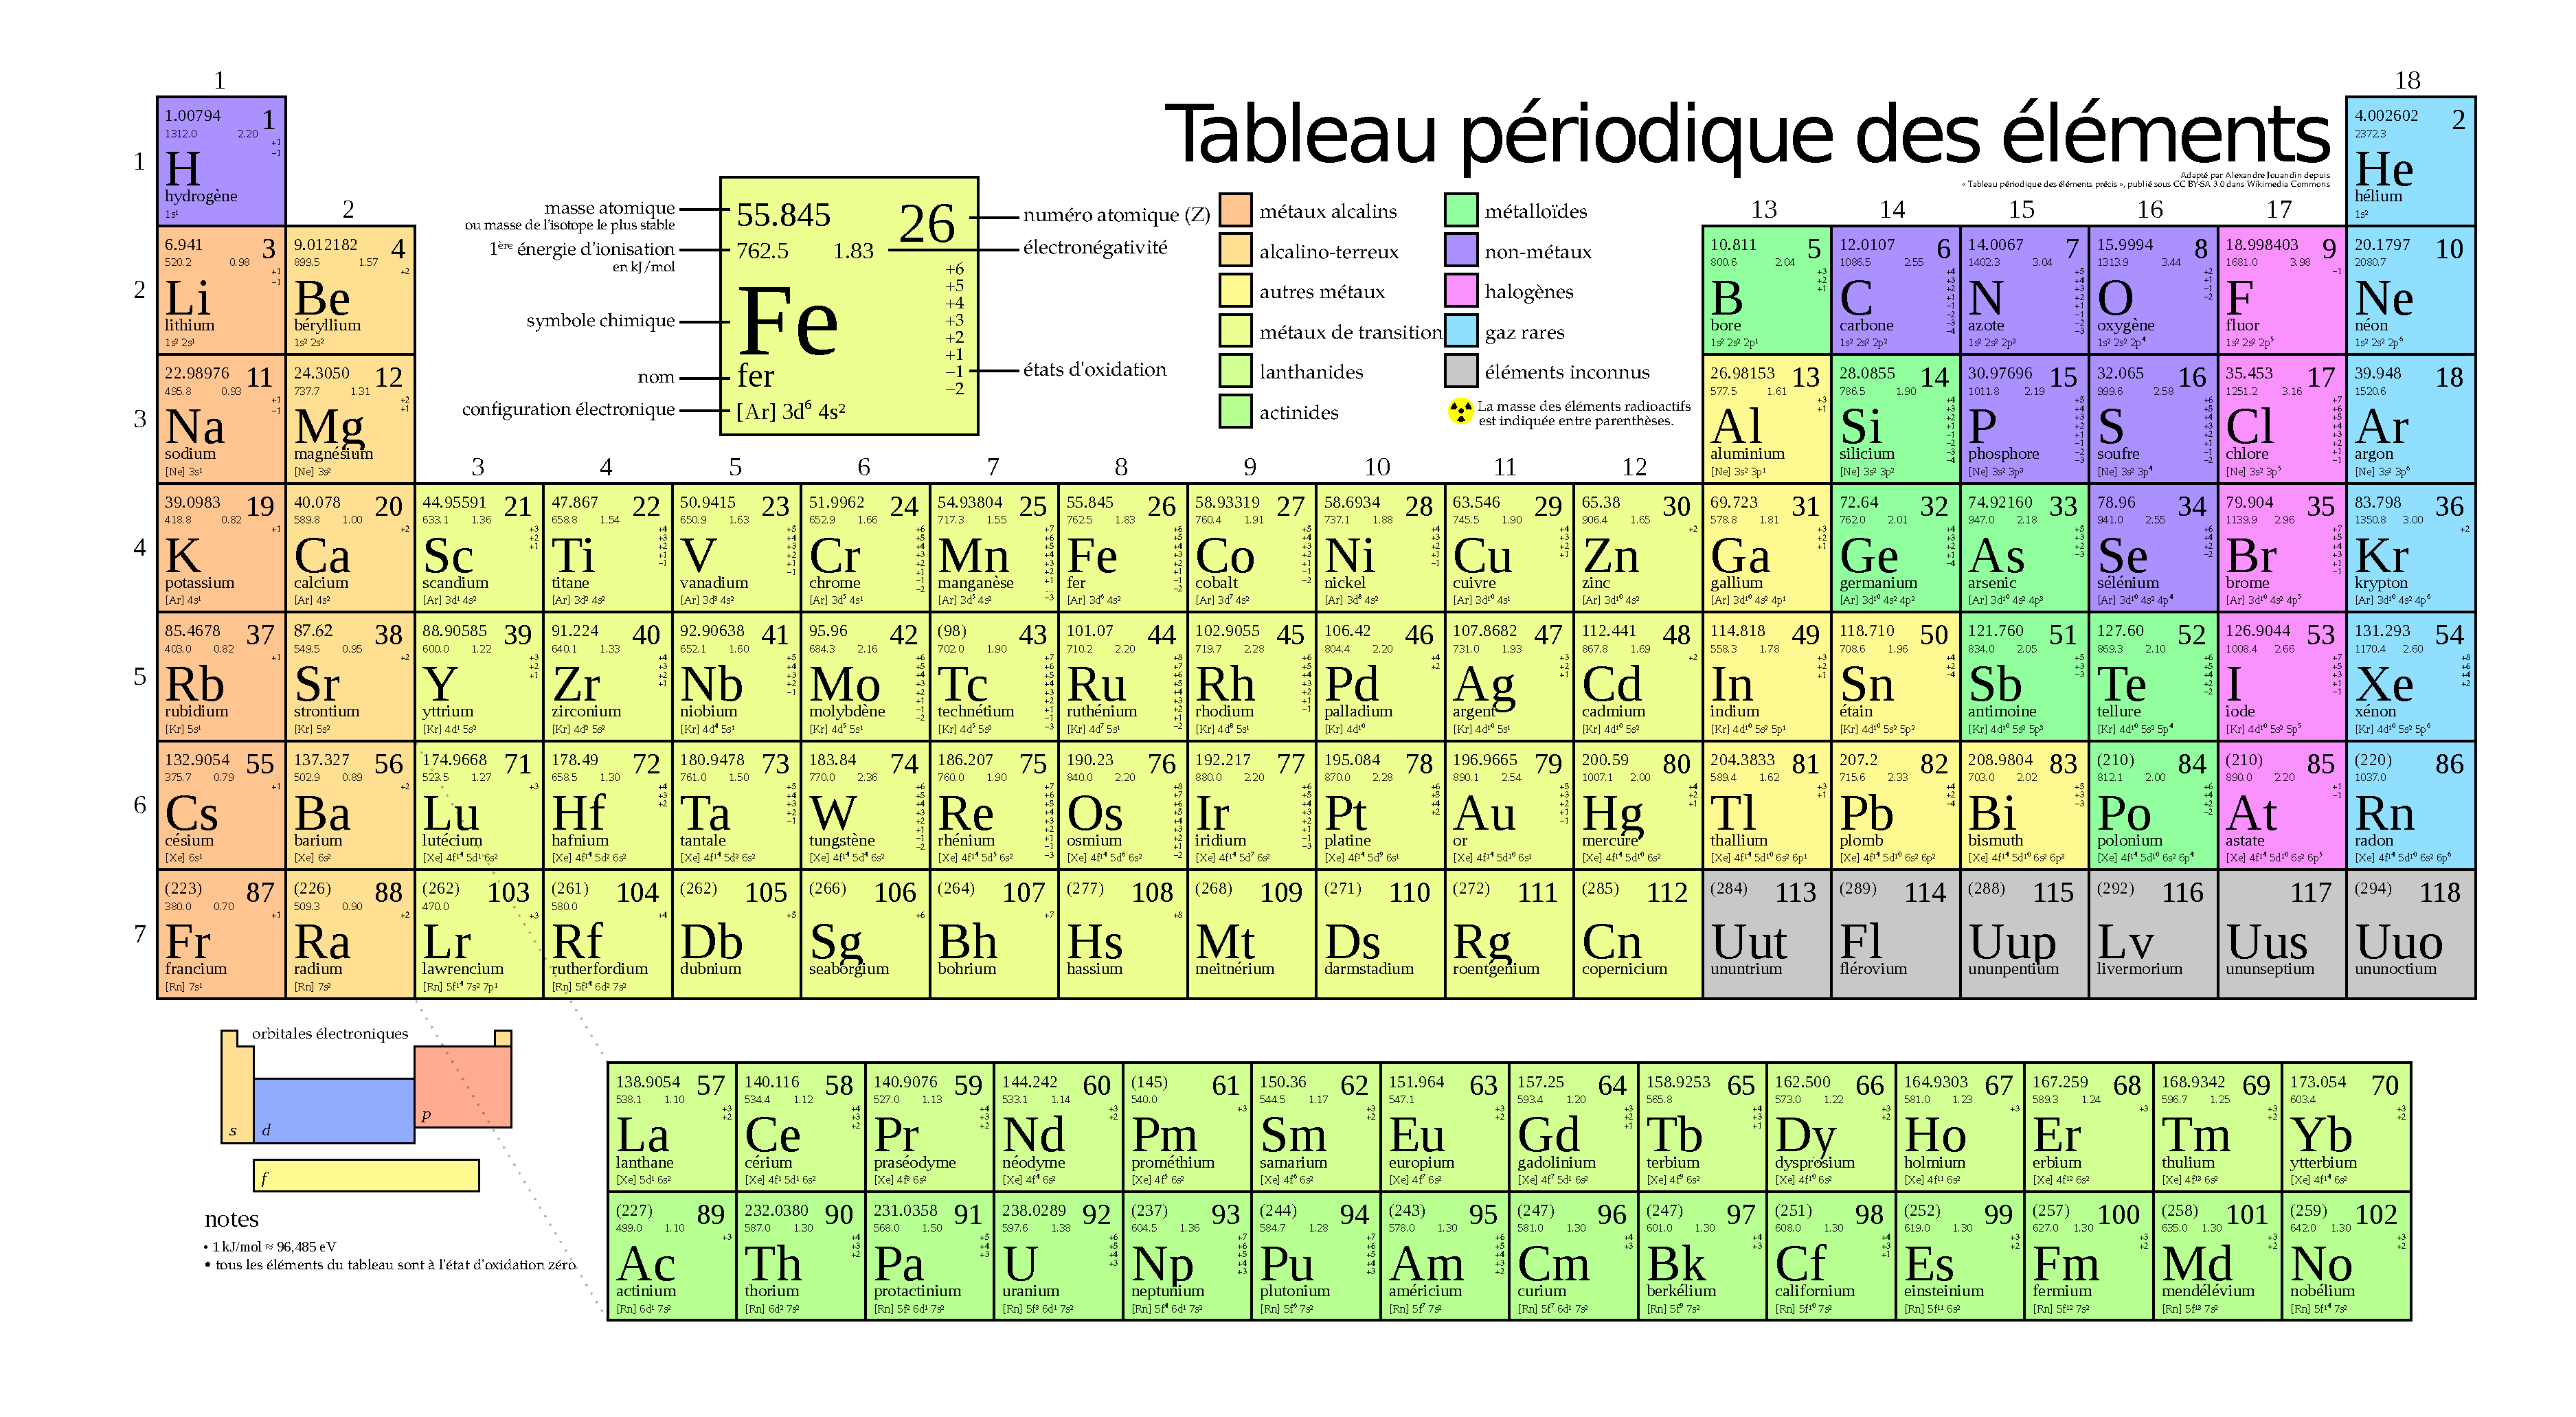
\includegraphics[keepaspectratio,width=\linewidth]{svg/tableau-periodique.pdf}
\begin{comment}
%% J'ai mis un tableau périodique en dessin Tikz pour au cas où. Et j'ai pas trop envie de supprimer son code... Merci Ivan Griffin en tout cas. 

%% Copyright 2009 Ivan Griffin
%
% This work may be distributed and/or modified under the
% conditions of the LaTeX Project Public License, either version 1.3
% of this license or (at your option) any later version.
% The latest version of this license is in
%   http://www.latex-project.org/lppl.txt
% and version 1.3 or later is part of all distributions of LaTeX
% version 2005/12/01 or later.
%
% This work has the LPPL maintenance status `maintained'.
% 
% The Current Maintainer of this work is Ivan Griffin
%
% This work consists of the files periodic_table.tex

%Description
%-----------
%periodic_table.tex - an example file illustrating the Periodic
%                     Table of Chemical Elements using TikZ

%Created 2009-12-08 by Ivan Griffin.  Last updated: 2010-01-11
%
%Thanks to Jerome
%-------------------------------------------------------------

\newcommand{\CommonElementTextFormat}[4]
{
  \begin{minipage}{2.2cm}
    \centering
      {\textbf{#1} \hfill #2}%
      \linebreak \linebreak
      {\textbf{#3}}%
      \linebreak \linebreak
      {{#4}}
  \end{minipage}
}

\newcommand{\NaturalElementTextFormat}[4]
{
  \CommonElementTextFormat{#1}{#2}{\LARGE {#3}}{#4}
}

\newcommand{\OutlineText}[1]
{
\ifpdf
  % Couldn't find a nicer way of doing an outline font with TikZ
  % other than using pdfliteral 1 Tr
  %
  \pdfliteral direct {0.5 w 1 Tr}{#1}%
  \pdfliteral direct {1 w 0 Tr}%
\else
  % pstricks can do this with \pscharpath from pstricks
  %
  \pscharpath[shadow=false,
    fillstyle=solid,
    fillcolor=white,
    linestyle=solid,
    linecolor=black,
    linewidth=.2pt]{#1} 
\fi
}

\newcommand{\SyntheticElementTextFormat}[4]
{
\ifpdf
  \CommonElementTextFormat{#1}{#2}{\OutlineText{\LARGE #3}}{#4}
\else
  % pstricks approach results in slightly larger box
  % that doesn't break, so fudge here
  \CommonElementTextFormat{#1}{#2}{\OutlineText{\Large #3}}{#4}
\fi
}

\begin{tikzpicture}[font=\sffamily, scale=0.5, transform shape]

%% Fill Color Styles
  \tikzstyle{ElementFill} = [fill=yellow!15]
  \tikzstyle{AlkaliMetalFill} = [fill=blue!55]
  \tikzstyle{AlkalineEarthMetalFill} = [fill=blue!40]
  \tikzstyle{MetalFill} = [fill=blue!25]
  \tikzstyle{MetalloidFill} = [fill=orange!25]
  \tikzstyle{NonmetalFill} = [fill=green!25]
  \tikzstyle{HalogenFill} = [fill=green!40]
  \tikzstyle{NobleGasFill} = [fill=green!55]
  \tikzstyle{LanthanideActinideFill} = [fill=purple!25]

%% Element Styles
  \tikzstyle{Element} = [draw=black, ElementFill,
    minimum width=2.75cm, minimum height=2.75cm, node distance=2.75cm]
  \tikzstyle{AlkaliMetal} = [Element, AlkaliMetalFill]
  \tikzstyle{AlkalineEarthMetal} = [Element, AlkalineEarthMetalFill]
  \tikzstyle{Metal} = [Element, MetalFill]
  \tikzstyle{Metalloid} = [Element, MetalloidFill]
  \tikzstyle{Nonmetal} = [Element, NonmetalFill]
  \tikzstyle{Halogen} = [Element, HalogenFill]
  \tikzstyle{NobleGas} = [Element, NobleGasFill]
  \tikzstyle{LanthanideActinide} = [Element, LanthanideActinideFill]
  \tikzstyle{PeriodLabel} = [font={\sffamily\LARGE}, node distance=2.0cm]
  \tikzstyle{GroupLabel} = [font={\sffamily\LARGE}, minimum width=2.75cm, node distance=2.0cm]
  \tikzstyle{TitleLabel} = [font={\sffamily\Huge\bfseries}]

%% Group 1 - IA
  \node[name=H, Element] {\NaturalElementTextFormat{1}{1.0079}{H}{Hydrogen}};
  \node[name=Li, below of=H, AlkaliMetal] {\NaturalElementTextFormat{3}{6.941}{Li}{Lithium}};
  \node[name=Na, below of=Li, AlkaliMetal] {\NaturalElementTextFormat{11}{22.990}{Na}{Sodium}};
  \node[name=K, below of=Na, AlkaliMetal] {\NaturalElementTextFormat{19}{39.098}{K}{Potassium}};
  \node[name=Rb, below of=K, AlkaliMetal] {\NaturalElementTextFormat{37}{85.468}{Rb}{Rubidium}};
  \node[name=Cs, below of=Rb, AlkaliMetal] {\NaturalElementTextFormat{55}{132.91}{Cs}{Caesium}};
  \node[name=Fr, below of=Cs, AlkaliMetal] {\NaturalElementTextFormat{87}{223}{Fr}{Francium}};

%% Group 2 - IIA
  \node[name=Be, right of=Li, AlkalineEarthMetal] {\NaturalElementTextFormat{4}{9.0122}{Be}{Beryllium}};
  \node[name=Mg, below of=Be, AlkalineEarthMetal] {\NaturalElementTextFormat{12}{24.305}{Mg}{Magnesium}};
  \node[name=Ca, below of=Mg, AlkalineEarthMetal] {\NaturalElementTextFormat{20}{40.078}{Ca}{Calcium}};
  \node[name=Sr, below of=Ca, AlkalineEarthMetal] {\NaturalElementTextFormat{38}{87.62}{Sr}{Strontium}};
  \node[name=Ba, below of=Sr, AlkalineEarthMetal] {\NaturalElementTextFormat{56}{137.33}{Ba}{Barium}};
  \node[name=Ra, below of=Ba, AlkalineEarthMetal] {\NaturalElementTextFormat{88}{226}{Ra}{Radium}};

%% Group 3 - IIIB
  \node[name=Sc, right of=Ca, Metal] {\NaturalElementTextFormat{21}{44.956}{Sc}{Scandium}};
  \node[name=Y, below of=Sc, Metal] {\NaturalElementTextFormat{39}{88.906}{Y}{Yttrium}};
  \node[name=LaLu, below of=Y, LanthanideActinide] {\NaturalElementTextFormat{57-71}{}{La-Lu}{Lanthanide}};
  \node[name=AcLr, below of=LaLu, LanthanideActinide] {\NaturalElementTextFormat{89-103}{}{Ac-Lr}{Actinide}};

%% Group 4 - IVB
  \node[name=Ti, right of=Sc, Metal] {\NaturalElementTextFormat{22}{47.867}{Ti}{Titanium}};
  \node[name=Zr, below of=Ti, Metal] {\NaturalElementTextFormat{40}{91.224}{Zr}{Zirconium}};
  \node[name=Hf, below of=Zr, Metal] {\NaturalElementTextFormat{72}{178.49}{Hf}{Halfnium}};
  \node[name=Rf, below of=Hf, Metal] {\SyntheticElementTextFormat{104}{261}{Rf}{Rutherfordium}};

%% Group 5 - VB
  \node[name=V, right of=Ti, Metal] {\NaturalElementTextFormat{23}{50.942}{V}{Vanadium}};
  \node[name=Nb, below of=V, Metal] {\NaturalElementTextFormat{41}{92.906}{Nb}{Niobium}};
  \node[name=Ta, below of=Nb, Metal] {\NaturalElementTextFormat{73}{180.95}{Ta}{Tantalum}};
  \node[name=Db, below of=Ta, Metal] {\SyntheticElementTextFormat{105}{262}{Db}{Dubnium}};

%% Group 6 - VIB
  \node[name=Cr, right of=V, Metal] {\NaturalElementTextFormat{24}{51.996}{Cr}{Chromium}};
  \node[name=Mo, below of=Cr, Metal] {\NaturalElementTextFormat{42}{95.94}{Mo}{Molybdenum}};
  \node[name=W, below of=Mo, Metal] {\NaturalElementTextFormat{74}{183.84}{W}{Tungsten}};
  \node[name=Sg, below of=W, Metal] {\SyntheticElementTextFormat{106}{266}{Sg}{Seaborgium}};

%% Group 7 - VIIB
  \node[name=Mn, right of=Cr, Metal] {\NaturalElementTextFormat{25}{54.938}{Mn}{Manganese}};
  \node[name=Tc, below of=Mn, Metal] {\NaturalElementTextFormat{43}{96}{Tc}{Technetium}};
  \node[name=Re, below of=Tc, Metal] {\NaturalElementTextFormat{75}{186.21}{Re}{Rhenium}};
  \node[name=Bh, below of=Re, Metal] {\SyntheticElementTextFormat{107}{264}{Bh}{Bohrium}};

%% Group 8 - VIIIB
  \node[name=Fe, right of=Mn, Metal] {\NaturalElementTextFormat{26}{55.845}{Fe}{Iron}};
  \node[name=Ru, below of=Fe, Metal] {\NaturalElementTextFormat{44}{101.07}{Ru}{Ruthenium}};
  \node[name=Os, below of=Ru, Metal] {\NaturalElementTextFormat{76}{190.23}{Os}{Osmium}};
  \node[name=Hs, below of=Os, Metal] {\SyntheticElementTextFormat{108}{277}{Hs}{Hassium}};

%% Group 9 - VIIIB
  \node[name=Co, right of=Fe, Metal] {\NaturalElementTextFormat{27}{58.933}{Co}{Cobalt}};
  \node[name=Rh, below of=Co, Metal] {\NaturalElementTextFormat{45}{102.91}{Rh}{Rhodium}};
  \node[name=Ir, below of=Rh, Metal] {\NaturalElementTextFormat{77}{192.22}{Ir}{Iridium}};
  \node[name=Mt, below of=Ir, Metal] {\SyntheticElementTextFormat{109}{268}{Mt}{Meitnerium}};

%% Group 10 - VIIIB
  \node[name=Ni, right of=Co, Metal] {\NaturalElementTextFormat{28}{58.693}{Ni}{Nickel}};
  \node[name=Pd, below of=Ni, Metal] {\NaturalElementTextFormat{46}{106.42}{Pd}{Palladium}};
  \node[name=Pt, below of=Pd, Metal] {\NaturalElementTextFormat{78}{195.08}{Pt}{Platinum}};
  \node[name=Ds, below of=Pt, Metal] {\SyntheticElementTextFormat{110}{281}{Ds}{Darmstadtium}};

%% Group 11 - IB
  \node[name=Cu, right of=Ni, Metal] {\NaturalElementTextFormat{29}{63.546}{Cu}{Copper}};
  \node[name=Ag, below of=Cu, Metal] {\NaturalElementTextFormat{47}{107.87}{Ag}{Silver}};
  \node[name=Au, below of=Ag, Metal] {\NaturalElementTextFormat{79}{196.97}{Au}{Gold}};
  \node[name=Rg, below of=Au, Metal] {\SyntheticElementTextFormat{111}{280}{Rg}{Roentgenium}};

%% Group 12 - IIB
  \node[name=Zn, right of=Cu, Metal] {\NaturalElementTextFormat{30}{65.39}{Zn}{Zinc}};
  \node[name=Cd, below of=Zn, Metal] {\NaturalElementTextFormat{48}{112.41}{Cd}{Cadmium}};
  \node[name=Hg, below of=Cd, Metal] {\NaturalElementTextFormat{80}{200.59}{Hg}{Mercury}};
  \node[name=Uub, below of=Hg, Metal] {\SyntheticElementTextFormat{112}{285}{Uub}{Ununbium}};

%% Group 13 - IIIA
  \node[name=Ga, right of=Zn, Metal] {\NaturalElementTextFormat{31}{69.723}{Ga}{Gallium}};
  \node[name=Al, above of=Ga, Metal] {\NaturalElementTextFormat{13}{26.982}{Al}{Aluminium}};
  \node[name=B, above of=Al, Metalloid] {\NaturalElementTextFormat{5}{10.811}{B}{Boron}};
  \node[name=In, below of=Ga, Metal] {\NaturalElementTextFormat{49}{114.82}{In}{Indium}};
  \node[name=Tl, below of=In, Metal] {\NaturalElementTextFormat{81}{204.38}{Tl}{Thallium}};
  \node[name=Uut, below of=Tl, Metal] {\SyntheticElementTextFormat{113}{284}{Uut}{Ununtrium}};

%% Group 14 - IVA
  \node[name=C, right of=B, Nonmetal] {\NaturalElementTextFormat{6}{12.011}{C}{Carbon}};
  \node[name=Si, below of=C, Metalloid] {\NaturalElementTextFormat{14}{28.086}{Si}{Silicon}};
  \node[name=Ge, below of=Si, Metalloid] {\NaturalElementTextFormat{32}{72.64}{Ge}{Germanium}};
  \node[name=Sn, below of=Ge, Metal] {\NaturalElementTextFormat{50}{118.71}{Sn}{Tin}};
  \node[name=Pb, below of=Sn, Metal] {\NaturalElementTextFormat{82}{207.2}{Pb}{Lead}};
  \node[name=Uuq, below of=Pb, Metal] {\SyntheticElementTextFormat{114}{289}{Uuq}{Ununquadium}};

%% Group 15 - VA
  \node[name=N, right of=C, Nonmetal] {\NaturalElementTextFormat{7}{14.007}{N}{Nitrogen}};
  \node[name=P, below of=N, Nonmetal] {\NaturalElementTextFormat{15}{30.974}{P}{Phosphorus}};
  \node[name=As, below of=P, Metalloid] {\NaturalElementTextFormat{33}{74.922}{As}{Arsenic}};
  \node[name=Sb, below of=As, Metalloid] {\NaturalElementTextFormat{51}{121.76}{Sb}{Antimony}};
  \node[name=Bi, below of=Sb, Metal] {\NaturalElementTextFormat{83}{208.98}{Bi}{Bismuth}};
  \node[name=Uup, below of=Bi, Metal] {\SyntheticElementTextFormat{115}{288}{Uup}{Ununpentium}};

%% Group 16 - VIA
  \node[name=O, right of=N, Nonmetal] {\NaturalElementTextFormat{8}{15.999}{O}{Oxygen}};
  \node[name=S, below of=O, Nonmetal] {\NaturalElementTextFormat{16}{32.065}{S}{Sulphur}};
  \node[name=Se, below of=S, Nonmetal] {\NaturalElementTextFormat{34}{78.96}{Se}{Selenium}};
  \node[name=Te, below of=Se, Metalloid] {\NaturalElementTextFormat{52}{127.6}{Te}{Tellurium}};
  \node[name=Po, below of=Te, Metalloid] {\NaturalElementTextFormat{84}{209}{Po}{Polonium}};
  \node[name=Uuh, below of=Po, Metal] {\SyntheticElementTextFormat{116}{293}{Uuh}{Ununhexium}};

%% Group 17 - VIIA
  \node[name=F, right of=O, Halogen] {\NaturalElementTextFormat{9}{18.998}{F}{Flourine}};
  \node[name=Cl, below of=F, Halogen] {\NaturalElementTextFormat{17}{35.453}{Cl}{Chlorine}};
  \node[name=Br, below of=Cl, Halogen] {\NaturalElementTextFormat{35}{79.904}{Br}{Bromine}};
  \node[name=I, below of=Br, Halogen] {\NaturalElementTextFormat{53}{126.9}{I}{Iodine}};
  \node[name=At, below of=I, Halogen] {\NaturalElementTextFormat{85}{210}{At}{Astatine}};
  \node[name=Uus, below of=At, Element] {\SyntheticElementTextFormat{117}{292}{Uus}{Ununseptium}}; 

%% Group 18 - VIIIA
  \node[name=Ne, right of=F, NobleGas] {\NaturalElementTextFormat{10}{20.180}{Ne}{Neon}};
  \node[name=He, above of=Ne, NobleGas] {\NaturalElementTextFormat{2}{4.0025}{He}{Helium}};
  \node[name=Ar, below of=Ne, NobleGas] {\NaturalElementTextFormat{18}{39.948}{Ar}{Argon}};
  \node[name=Kr, below of=Ar, NobleGas] {\NaturalElementTextFormat{36}{83.8}{Kr}{Krypton}};
  \node[name=Xe, below of=Kr, NobleGas] {\NaturalElementTextFormat{54}{131.29}{Xe}{Xenon}};
  \node[name=Rn, below of=Xe, NobleGas] {\NaturalElementTextFormat{86}{222}{Rn}{Radon}};
  \node[name=Uuo, below of=Rn, Nonmetal] {\SyntheticElementTextFormat{118}{294}{Uuo}{Ununoctium}}; 

%% Period
  \node[name=Period1, left of=H, PeriodLabel] {1};
  \node[name=Period2, left of=Li, PeriodLabel] {2};
  \node[name=Period3, left of=Na, PeriodLabel] {3}; 
  \node[name=Period4, left of=K, PeriodLabel] {4}; 
  \node[name=Period5, left of=Rb, PeriodLabel] {5};
  \node[name=Period6, left of=Cs, PeriodLabel] {6};
  \node[name=Period7, left of=Fr, PeriodLabel] {7};

%% Group
  \node[name=Group1, above of=H, GroupLabel] {1 \hfill IA};
  \node[name=Group2, above of=Be, GroupLabel] {2 \hfill IIA};
  \node[name=Group3, above of=Sc, GroupLabel] {3 \hfill IIIA};
  \node[name=Group4, above of=Ti, GroupLabel] {4 \hfill IVB};
  \node[name=Group5, above of=V, GroupLabel] {5 \hfill VB};
  \node[name=Group6, above of=Cr, GroupLabel] {6 \hfill VIB};
  \node[name=Group7, above of=Mn, GroupLabel] {7 \hfill VIIB};
  \node[name=Group8, above of=Fe, GroupLabel] {8 \hfill VIIIB};
  \node[name=Group9, above of=Co, GroupLabel] {9 \hfill VIIIB};
  \node[name=Group10, above of=Ni, GroupLabel] {10 \hfill VIIIB};
  \node[name=Group11, above of=Cu, GroupLabel] {11 \hfill IB};
  \node[name=Group12, above of=Zn, GroupLabel] {12 \hfill IIB};
  \node[name=Group13, above of=B, GroupLabel] {13 \hfill IIIA};
  \node[name=Group14, above of=C, GroupLabel] {14 \hfill IVA};
  \node[name=Group15, above of=N, GroupLabel] {15 \hfill VA};
  \node[name=Group16, above of=O, GroupLabel] {16 \hfill VIA};
  \node[name=Group17, above of=F, GroupLabel] {17 \hfill VIIA};
  \node[name=Group18, above of=He, GroupLabel] {18 \hfill VIIIA};

%% Lanthanide
  \node[name=La, below of=Rf, LanthanideActinide, yshift=-1cm] {\NaturalElementTextFormat{57}{138.91}{La}{Lanthanum}};
  \node[name=Ce, right of=La, LanthanideActinide] {\NaturalElementTextFormat{58}{140.12}{Ce}{Cerium}};
  \node[name=Pr, right of=Ce, LanthanideActinide] {\NaturalElementTextFormat{59}{140.91}{Pr}{Praseodymium}};
  \node[name=Nd, right of=Pr, LanthanideActinide] {\NaturalElementTextFormat{60}{144.24}{Nd}{Neodymium}};
  \node[name=Pm, right of=Nd, LanthanideActinide] {\NaturalElementTextFormat{61}{145}{Pm}{Promethium}};
  \node[name=Sm, right of=Pm, LanthanideActinide] {\NaturalElementTextFormat{62}{150.36}{Sm}{Samarium}};
  \node[name=Eu, right of=Sm, LanthanideActinide] {\NaturalElementTextFormat{63}{151.96}{Eu}{Europium}};
  \node[name=Gd, right of=Eu, LanthanideActinide] {\NaturalElementTextFormat{64}{157.25}{Gd}{Gadolinium}};
  \node[name=Tb, right of=Gd, LanthanideActinide] {\NaturalElementTextFormat{65}{158.93}{Tb}{Terbium}};
  \node[name=Dy, right of=Tb, LanthanideActinide] {\NaturalElementTextFormat{66}{162.50}{Dy}{Dysprosium}};
  \node[name=Ho, right of=Dy, LanthanideActinide] {\NaturalElementTextFormat{67}{164.93}{Ho}{Holmium}};
  \node[name=Er, right of=Ho, LanthanideActinide] {\NaturalElementTextFormat{68}{167.26}{Er}{Erbium}};
  \node[name=Tm, right of=Er, LanthanideActinide] {\NaturalElementTextFormat{69}{168.93}{Tm}{Thulium}};
  \node[name=Yb, right of=Tm, LanthanideActinide] {\NaturalElementTextFormat{70}{173.04}{Yb}{Ytterbium}};
  \node[name=Lu, right of=Yb, LanthanideActinide] {\NaturalElementTextFormat{71}{174.97}{Lu}{Lutetium}};

%% Actinide
  \node[name=Ac, below of=La, LanthanideActinide, yshift=-1cm] {\NaturalElementTextFormat{89}{227}{Ac}{Actinium}};
  \node[name=Th, right of=Ac, LanthanideActinide] {\NaturalElementTextFormat{90}{232.04}{Th}{Thorium}};
  \node[name=Pa, right of=Th, LanthanideActinide] {\NaturalElementTextFormat{91}{231.04}{Pa}{Protactinium}};
  \node[name=U, right of=Pa, LanthanideActinide] {\NaturalElementTextFormat{92}{238.03}{U}{Uranium}};
  \node[name=Np, right of=U, LanthanideActinide] {\SyntheticElementTextFormat{93}{237}{Np}{Neptunium}};
  \node[name=Pu, right of=Np, LanthanideActinide] {\SyntheticElementTextFormat{94}{244}{Pu}{Plutonium}};
  \node[name=Am, right of=Pu, LanthanideActinide] {\SyntheticElementTextFormat{95}{243}{Am}{Americium}};
  \node[name=Cm, right of=Am, LanthanideActinide] {\SyntheticElementTextFormat{96}{247}{Cm}{Curium}};
  \node[name=Bk, right of=Cm, LanthanideActinide] {\SyntheticElementTextFormat{97}{247}{Bk}{Berkelium}};
  \node[name=Cf, right of=Bk, LanthanideActinide] {\SyntheticElementTextFormat{98}{251}{Cf}{Californium}};
  \node[name=Es, right of=Cf, LanthanideActinide] {\SyntheticElementTextFormat{99}{252}{Es}{Einsteinium}};
  \node[name=Fm, right of=Es, LanthanideActinide] {\SyntheticElementTextFormat{100}{257}{Fm}{Fermium}};
  \node[name=Md, right of=Fm, LanthanideActinide] {\SyntheticElementTextFormat{101}{258}{Md}{Mendelevium}};
  \node[name=No, right of=Md, LanthanideActinide] {\SyntheticElementTextFormat{102}{259}{No}{Nobelium}};
  \node[name=Lr, right of=No, LanthanideActinide] {\SyntheticElementTextFormat{103}{262}{Lr}{Lawrencium}};

%% Draw dotted lines connecting Lanthanide breakout to main table
  \draw (LaLu.north west) edge[dotted] (La.north west)
        (LaLu.north east) edge[dotted] (Lu.north east)
        (LaLu.south west) edge[dotted] (La.south west)
        (LaLu.south east) edge[dotted] (Lu.south east);
%% Draw dotted lines connecting Actinide breakout to main table
  \draw (AcLr.north west) edge[dotted] (Ac.north west)
        (AcLr.north east) edge[dotted] (Lr.north east)
        (AcLr.south west) edge[dotted] (Ac.south west)
        (AcLr.south east) edge[dotted] (Lr.south east);

%% Legend
  \draw[black, AlkaliMetalFill] ($(La.north -| Fr.west) + (1em,-0.0em)$)
    rectangle +(1em, 1em) node[right, yshift=-1ex]{Métaux alcalins};
  \draw[black, AlkalineEarthMetalFill] ($(La.north -| Fr.west) + (1em,-1.5em)$)
    rectangle +(1em, 1em) node[right, yshift=-1ex]{Métaux alcalino-terreux};
  \draw[black, MetalFill] ($(La.north -| Fr.west) + (1em,-3.0em)$)
    rectangle +(1em, 1em) node[right, yshift=-1ex]{Autres métaux};
  \draw[black, MetalloidFill] ($(La.north -| Fr.west) + (1em,-4.5em)$)
    rectangle +(1em, 1em) node[right, yshift=-1ex]{Metalloid};
  \draw[black, NonmetalFill] ($(La.north -| Fr.west) + (1em,-6.0em)$)
    rectangle +(1em, 1em) node[right, yshift=-1ex]{Non-metal};
  \draw[black, HalogenFill] ($(La.north -| Fr.west) + (1em,-7.5em)$)
    rectangle +(1em, 1em) node[right, yshift=-1ex]{Halogen};
  \draw[black, NobleGasFill] ($(La.north -| Fr.west) + (1em,-9.0em)$)
    rectangle +(1em, 1em) node[right, yshift=-1ex]{Noble Gas};
  \draw[black, LanthanideActinideFill] ($(La.north -| Fr.west) + (1em,-10.5em)$)
    rectangle +(1em, 1em) node[right, yshift=-1ex]{Lanthanide/Actinide};

  \node at ($(La.north -| Fr.west) + (5em,-15em)$) [name=elementLegend, Element, fill=white]
    {\NaturalElementTextFormat{Z}{masse}{Symbole}{Nom}};
  \node[Element, fill=white, right of=elementLegend, xshift=1em]
    {\SyntheticElementTextFormat{}{}{ar\-ti\-fi\-ciel}{}} ;

%% Diagram Title
  \node at (H.west -| Fe.north) [name=diagramTitle, TitleLabel]
    {Tableau périodique des éléments de \textsc{Mendeleev}};

\end{tikzpicture}
\end{comment}
\caption{Tableau périodique des éléments de \textsc{Mendeleev}}
\end{figure}
\ifoptionfinal{\end{landscape}}{}
\newgeometry{left=3cm,bottom=5cm,right=3cm,top=5cm} % On restaure la géometrie initiale
% chapter annexe_chimie (end)
% part chimie (end)
\printnoidxglossary[type=\acronymtype,style=longragged,title={Liste des acronymes}]
\printindex{}
\end{document}
%